% A LaTeX template for MSc Thesis submissions to
% Politecnico di Milano (PoliMi) - School of Industrial and Information Engineering
%
% S. Bonetti, A. Gruttadauria, G. Mescolini, A. Zingaro
% e-mail: template-tesi-ingind@polimi.it
%
% Last Revision: October 2021
%
% Copyright 2021 Politecnico di Milano, Italy. NC-BY

\documentclass{Configuration_Files/PoliMi3i_thesis}

%------------------------------------------------------------------------------
%	REQUIRED PACKAGES AND  CONFIGURATIONS
%------------------------------------------------------------------------------

% CONFIGURATIONS
\usepackage{parskip} % For paragraph layout
\usepackage{setspace} % For using single or double spacing
\usepackage{emptypage} % To insert empty pages
\usepackage{multicol} % To write in multiple columns (executive summary)
\setlength\columnsep{15pt} % Column separation in executive summary
\setlength\parindent{0pt} % Indentation
\raggedbottom

% PACKAGES FOR TITLES
\usepackage{titlesec}
\titlespacing{\section}{0pt}{3.3ex}{2ex}
\titlespacing{\subsection}{0pt}{3.3ex}{1.65ex}
\titlespacing{\subsubsection}{0pt}{3.3ex}{1ex}
\usepackage{color}

% PACKAGES FOR LANGUAGE AND FONT
\usepackage[english]{babel} % The document is in English
\usepackage[utf8]{inputenc} % UTF8 encoding
\usepackage[T1]{fontenc} % Font encoding
\usepackage[11pt]{moresize} % Big fonts

% PACKAGES FOR IMAGES
\usepackage{graphicx}
\usepackage{transparent} % Enables transparent images
\usepackage{eso-pic} % For the background picture on the title page
\usepackage{subfig} % Numbered and caption subfigures using \subfloat.
\usepackage{tikz} % A package for high-quality hand-made figures.
\usetikzlibrary{}
\graphicspath{{./Images/}} % Directory of the images
\usepackage{amsthm,thmtools,xcolor} % Coloured "Theorem"
\usepackage{float}

% STANDARD MATH PACKAGES
\usepackage{amsmath}
\usepackage{amssymb}
\usepackage{amsfonts}
\usepackage{bm}
\usepackage[overload]{empheq} % For braced-style systems of equations.
\usepackage{fix-cm} % To override original LaTeX restrictions on sizes

% PACKAGES FOR TABLES
\usepackage{tabularx}
\usepackage{longtable} % Tables that can span several pages
\usepackage{colortbl}

% PACKAGES FOR ALGORITHMS (PSEUDO-CODE)
\usepackage{algorithm}
\usepackage{algorithmic}

% PACKAGES FOR REFERENCES & BIBLIOGRAPHY
\usepackage[colorlinks=true,linkcolor=black,anchorcolor=black,citecolor=black,filecolor=black,menucolor=black,runcolor=black,urlcolor=black]{hyperref} % Adds clickable links at references
\usepackage{cleveref}
\usepackage[square, numbers, sort&compress]{natbib} % Square brackets, citing references with numbers, citations sorted by appearance in the text and compressed
\bibliographystyle{abbrvnat} % You may use a different style adapted to your field

% OTHER PACKAGES
\usepackage{listings}
\usepackage{pdfpages} % To include a pdf file
\usepackage{afterpage}
\usepackage{lipsum} % DUMMY PACKAGE
\usepackage{fancyhdr} % For the headers
\usepackage{minted}

% Input of configuration file. Do not change config.tex file unless you really know what you are doing.
% Define blue color typical of polimi
\definecolor{bluepoli}{cmyk}{0.4,0.1,0,0.4}%

% Custom theorem environments
\declaretheoremstyle[%
    headfont=\color{bluepoli}\normalfont\bfseries,
    bodyfont=\color{black}\normalfont\itshape,
]{colored}%

% Set-up caption colors
\captionsetup[figure]{labelfont={color=bluepoli}}% % Set colour of the captions
\captionsetup[table]{labelfont={color=bluepoli}}% % Set colour of the captions
\captionsetup[algorithm]{labelfont={color=bluepoli}}% % Set colour of the captions

\theoremstyle{colored}%
\newtheorem{theorem}{Theorem}[chapter]%
\newtheorem{proposition}{Proposition}[chapter]%

% Enhances the features of the standard "table" and "tabular" environments.
\newcommand\T{\rule{0pt}{2.6ex}}%
\newcommand\B{\rule[-1.2ex]{0pt}{0pt}}%

% Pseudo-code algorithm descriptions.
\newcounter{algsubstate}%
\renewcommand{\thealgsubstate}{\alph{algsubstate}}%
\newenvironment{algsubstates}%
{\setcounter{algsubstate}{0}%
\renewcommand{\STATE}{%
    \stepcounter{algsubstate}%
    \Statex{\small\thealgsubstate:}\space}}%
{}%

% New font size
\newcommand\numfontsize{\@setfontsize\Huge{200}{60}}%

% Title format: chapter
\titleformat{\chapter}[hang]{%
    \fontsize{50}{20}\selectfont\bfseries\filright}{\textcolor{bluepoli}\thechapter\hsp\hspace{2mm}\textcolor{bluepoli}{|   }\hsp}{0pt}{\huge\bfseries\textcolor{bluepoli}%
}%

% Title format: section
\titleformat{\section}%
{\color{bluepoli}\normalfont\Large\bfseries}%
{\color{bluepoli}\thesection.}{1em}{}%

% Title format: subsection
\titleformat{\subsection}%
{\color{bluepoli}\normalfont\large\bfseries}%
{\color{bluepoli}\thesubsection.}{1em}{}%

% Title format: subsubsection
\titleformat{\subsubsection}%
{\color{bluepoli}\normalfont\large\bfseries}%
{\color{bluepoli}\thesubsubsection.}{1em}{}%

% Shortening for setting no horizontal-spacing
\newcommand{\hsp}{\hspace{0pt}}%

\makeatletter
% Renewcommand: cleardoublepage including the background pic
\renewcommand*\cleardoublepage{%
    \clearpage\if@twoside\ifodd\c@page\else
    \null
    \AddToShipoutPicture*{\BackgroundPic}%
    \thispagestyle{empty}%
    \newpage
    \if@twocolumn\hbox{}\newpage\fi\fi\fi}%
\makeatother

%For correctly numbering algorithms
\numberwithin{algorithm}{chapter}%


%----------------------------------------------------------------------------
%	NEW COMMANDS DEFINED
%----------------------------------------------------------------------------

%----------------------------------------------------------------------------
%	ADD YOUR PACKAGES (be careful of package interaction)
%----------------------------------------------------------------------------

%----------------------------------------------------------------------------
%	ADD YOUR DEFINITIONS AND COMMANDS (be careful of existing commands)
%----------------------------------------------------------------------------

%----------------------------------------------------------------------------
%	BEGIN OF YOUR DOCUMENT
%----------------------------------------------------------------------------
\begin{document}
    \fancypagestyle{plain}{%
        \fancyhf{} % Clear all header and footer fields
        \fancyhead[RO,RE]{\thepage} %RO=right odd, RE=right even
        \renewcommand{\headrulewidth}{0pt}
        \renewcommand{\footrulewidth}{0pt}}

%----------------------------------------------------------------------------
%	TITLE PAGE
%----------------------------------------------------------------------------

    \pagestyle{empty} % No page numbers
    \frontmatter % Use roman page numbering style (i, ii, iii, iv...) for the preamble pages

    \puttitle{
        title=Systems and Methods for Big and Unstructured Data Project,
        name1=Fabio Lusha - 10882532, % Author Name and Surname
        name2=Enrico Simionato - 10698193,
        name3=Irfan Cela - 10694934,
        name4=Bianca C. Savoiu Marinas - 10684465,
        name5=Alberto Sandri - 10698469,
        academicyear=2022-2023,
        groupnumber=31
    } % These info will be put into your Title page

%----------------------------------------------------------------------------
%	PREAMBLE PAGES: ABSTRACT (inglese e italiano), EXECUTIVE SUMMARY
%----------------------------------------------------------------------------
    \startpreamble
    \setcounter{page}{1} % Set page counter to 1

%----------------------------------------------------------------------------
%	LIST OF CONTENTS/FIGURES/TABLES/SYMBOLS
%----------------------------------------------------------------------------

% TABLE OF CONTENTS
    \thispagestyle{empty}
    \tableofcontents % Table of contents
    \thispagestyle{empty}
    \cleardoublepage

%-------------------------------------------------------------------------
%	THESIS MAIN TEXT
%-------------------------------------------------------------------------
% In the main text of your thesis you can write the chapters in two different ways:
%
%(1) As presented in this template you can write:
%    \chapter{Title of the chapter}
%    *body of the chapter*
%
%(2) You can write your chapter in a separated .tex file and then include it in the main file with the following command:
%    \chapter{Title of the chapter}
%    \input{chapter_file.tex}
%
% Especially for long thesis, we recommend you the second option.

    \addtocontents{toc}{\vspace{2em}} % Add a gap in the Contents, for aesthetics
    \mainmatter % Begin numeric (1,2,3...) page numbering

    \definecolor{codegreen}{rgb}{0,0.6,0}
    \definecolor{codegray}{rgb}{0.5,0.5,0.5}
    \definecolor{codepurple}{rgb}{0.58,0,0.82}
    \definecolor{backcolour}{rgb}{0.95,0.95,0.92}

    \lstdefinestyle{mystyle}{
        backgroundcolor=\color{backcolour},
        commentstyle=\color{codegreen},
        keywordstyle=\color{magenta},
        numberstyle=\tiny\color{codegray},
        stringstyle=\color{codepurple},
        basicstyle=\ttfamily\footnotesize,
        breakatwhitespace=false,
        breaklines=true,
        captionpos=b,
        keepspaces=true,
        numbers=left,
        numbersep=5pt,
        showspaces=false,
        showstringspaces=false,
        showtabs=false,
        tabsize=2
    }
    \lstset{language=SQL, style=mystyle}


    \part{Introduction}
    \label{part:introduction}%
    \chapter{Introduction to the problem}
\label{ch:chapter_one}%


\section{Problem description}
\label{sec:section_name}%
Scientific research is the engine that leads us through the future providing the technology to improve every single detail of our life.
Nowadays, the speed at which humanity and technology advance is outstanding thanks to scientists' progress in their fields of study.
The reaching of new results in the research materializes through scientific articles.
Since the advent of the World Wide Web, publishers started to post their papers on the net reaching an audience far larger than before.
This has allowed a more convenient and faster way to share knowledge, therefore boosting academic research and consequently the publishing of new papers.
Researchers need to navigate and access this massive quantity of knowledge, which is growing every day, thus, if we want to bolster human progress, new methods of organizing and managing these data are mandatory.


\section{Purpose}
\label{sec:purpose}%
The purpose of the project is to create a bibliographic database, namely a system able to store and manage data regarding scientific articles and all their meaningful characteristics and relations with authors and the place where they are published.


\section{Assumptions and important concepts}
\label{sec:assumptions_and_important_concepts}%
The problem we are addressing is very wide, and given the heterogeneity of the data different assumptions can be made.
We shaped our database by taking into consideration the following aspects:
\begin{itemize}
    \item A scientific paper can be written by one or more authors;
    \item All the authors of a paper are considered to be at the same level, so the position of coauthor is not considered;
    \item The papers the system considers were published in journals, books or were presented at conferences;
    \item A paper can appear in just one publication among journals, books, and conferences;
    \item A single affiliation of an author can be registered when a paper is written;
    \item Papers can have multiple fields of study (fos) and keywords;
    \item Not every paper has to be related to a field of study;
    \item Not every paper has to have related keywords;
    \item The name of the author may be complete or abbreviated;
    \item A paper may or may not reference other papers or be referenced by others.
\end{itemize}


\chapter{ER model}
\label{ch:er_model}%
As a bibliographic database, the main focus is on scientific articles, also called scientific papers, that can be considered the central entity.
Every article is written by one or more authors and each writer is associated with an organization.
Articles have several features like title, year of publication, language, abstract, DOI, and URL and can have many keywords and can be related to many fields of study.
Furthermore, a paper can reference other papers, and each article is published in a book, in a journal, or presented during a conference.

The place where an article is published is called in a general way \textit{publication} and each one of them has different properties: conferences take place in a specific location, books have an ISBN and a publisher, and journals have an ISSN, volume, issue and a publisher.
So the \verb|Publication| entity is extended with a hierarchy that is total and exclusive: a node has to be instantiated as one of the specific types of publication and cannot be more than one type at a time.

The group opted for a straightforward model with only the core concepts and relationships to make it easily understandable and represent it concisely.
Of course, the problem domain is very wide and complex but in this modeling phase, it was taken into account also the available data to build the model, trying to leave it quite general so that it would be easier to modify it and make it more complex in further versions.

In the following ER model, we chose to represent the cardinalities of the relationships always starting from one, so we don't consider entities that are not related to others.
When adding data to the database we can have, in an initial state, some isolated nodes, but in the ER we show a stable and correct state of the system.

As we can see from the diagram, we use in general the attribute \verb|id| as an identifier of the entities, but in some cases in the real world, there are better options, for instance, the \verb|Book| might be identified by the attribute \verb|ISBN|.
We made this assumption because our dataset was not complete, and a lot of \verb|Book| entities didn't have this property.
The same reasoning can be applied to \verb|Paper| with \verb|DOI|, \verb|Journal| with \verb|ISSN|, and \verb|Author| with \verb|ORCiD| that we disregarded because not present in the used data file.
\begin{figure}[H]
    \begin{center}
        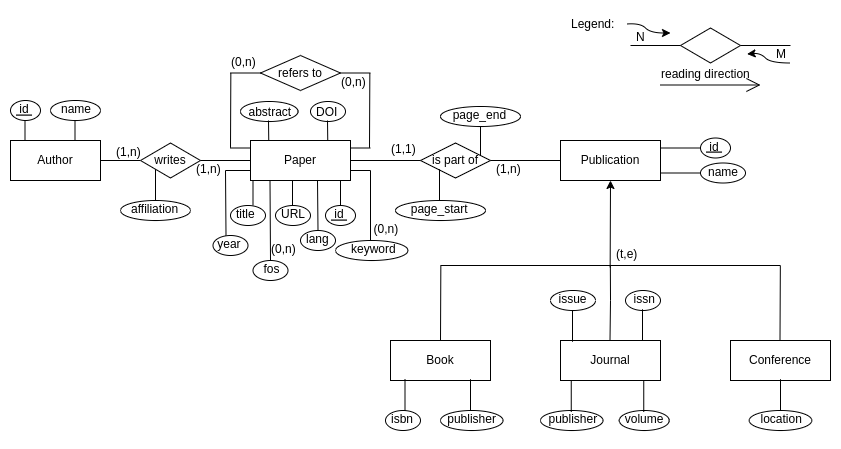
\includegraphics[width=0.9\textwidth]{Images/er}
        \caption{ER model of the bibliographic database.}
        \label{fig:er}%
    \end{center}
\end{figure}

\paragraph{More detailed description of entities}
\begin{itemize}
    \item \textbf{Paper}, as said before, is the most important entity, indeed it is in the middle of the model.
    Each paper is characterized by an ID, a title, a publication year, an abstract, a list of keywords, a list of fields of study, a DOI which is a unique global identifier, and a URL to reach the site where it is available for consultation.
    \item \textbf{Author} of a paper is identified by an ID and has a name, that contains both the name and the surname of the author.
    \item \textbf{Publication} is a total and exclusive hierarchy that represents the physical place where a paper is published, it has an ID and a name called the venue, and it is specialized in:
    \begin{itemize}
        \item \textbf{Conference} that has a location where it took place;
        \item \textbf{Book} that has a global identifier called ISBN and a publisher;
        \item \textbf{Journal} that has a global identifier called ISSN, a publisher,
        a volume and issue.
    \end{itemize}
\end{itemize}

\paragraph{More detailed description of relationships}
\begin{itemize}
    \item \textbf{WRITES} links Author and Paper, each author can write one or more papers, and each paper is written by one or more authors.
    This relationship has an attribute affiliation that is the organization the author was part of when the article was written.
    \item \textbf{REFERS TO} links two Paper entities, each paper can reference many papers and can be referenced by many papers.
    \item \textbf{IS PART OF} links Paper and Publication, each paper is published on a single publication and each publication can contain several papers.
    This relationship has as attributes the page\_start and page\_end of the article within the publication.
\end{itemize}

\paragraph{More detailed observations}
\begin{itemize}
    \item DOI could have been a good identifier for papers since it is globally unique, but in the used dataset not all articles had it.
    \item ORCiD is a unique identifier for authors that would have been a valid key for the entity Author but this data was not present in the used dataset.
    \item Since the focus is on the entity Paper and a simple model for the domain was built, it seemed not meaningful to have a separate entity to model the organization whose author is part of.
    In addition, that would have had just one attribute.
    For this reason, the concept of affiliation was modeled as an attribute of the relationship WRITES, storing multiple affiliations for the single author.
\end{itemize}



    \part{Neo4j}
    \label{part:neo4j}%
    \chapter{Dataset description}
\label{ch:dataset_description_neo4j}%
The main dataset used can be downloaded from the site \href{https://www.aminer.org/citation}{www.aminer.org}, in particular, the latest version of data was employed, namely DBLP-Citation network V13.
The dataset was not entirely imported in Neo4j because it was huge and our machines with limited computing power were not able to handle it, so just a part of it was taken, containing information about 2315 papers.

The following table shows the dataset's fields that were used, associated with their respective meaning, name, and role in the created database.
The fields publisher and location were not present in the original dataset, that's why we created this information from scratch, but this aspect is further discussed in the following chapter.
\begin{table}[H]
    \centering
    \begin{tabular}{| c | c | c | c | c |}
        \hline
        \textbf{Field name} & \textbf{Type} & \textbf{Description} & \textbf{Name in Neo4j} & \textbf{Usage in Neo4j}  \T\B \\
        \hline
        \hline
        \_id                & String        & paper ID             & id                     & node Paper\T\B              \\
        title               & String        & paper title          & title                  & node Paper\T\B              \\
        year                & Integer       & paper year           & year                   & node Paper\T\B              \\
        lang                & String        & paper language       & lang                   & node Paper\T\B              \\
        doi                 & String        & paper DOI            & doi                    & node Paper\T\B              \\
        url                 & String        & paper URL            & url                    & node Paper\T\B              \\
        abstract            & String        & paper abstract       & abstract               & node Paper \T\B             \\
        keywords[i]         & String        & paper keyword        & keyword                & node Keyword\T\B            \\
        fos[i]              & String        & paper field of study & fos                    & node Fos\T\B                \\
        references[i]       & String        & paper reference      & REFERENCES             & relation REFERENCES\T\B     \\
        page\_start         & Integer       & start page           & page\_start            & attribute IS\_PART\_OF \T\B \\
        page\_end           & Integer       & end page             & page\_end              & attribute IS\_PART\_OF \T\B \\
        authors.\_id        & String        & author ID            & id                     & node Author\T\B             \\
        authors.name        & String        & author name          & name                   & node Author\T\B             \\
        authors.org         & String        & author affiliation   & affiliation            & attribute WRITES\T\B        \\
        venue.raw           & String        & publication name     & name                   & node Publication \T\B       \\
        isbn                & String        & book ISBN            & isbn                   & node Book \T\B              \\
        publisher           & String        & publisher name       & publisher              & node Book/Journal \T\B      \\
        issn                & String        & journal ISSN         & issn                   & node Journal \T\B           \\
        volume              & String        & journal volume       & volume                 & node Journal \T\B           \\
        issue               & String        & journal issue        & issue                  & node Journal \T\B           \\
        location            & String        & conference location  & location               & node Conference \T\B        \\
        \hline
    \end{tabular}
    \\[8pt]
    \caption{Description of the data used in the project and relationship between original dataset and imported data.}
    \label{tab:dataset_description}%
\end{table}


\chapter{Data upload}
\label{ch:data_upload_neo4j}%


\section{Pre-processing}
\label{sec:pre_processing_neo4j}%
Before uploading the data in Neo4j, the dataset was downloaded from the website mentioned above, and just a part of it has been extracted.
Then some ad-hoc Python scripts have been used to do a first-level cleaning of the data since we found some inconsistency in it.
Specifically, the cleaning involved the following aspects:
\begin{itemize}
    \item Some numerical attributes were wrapped in NumberInt(\ldots) string.
    This is not a standard way to store numeric values in JSON so it couldn't be parsed by the Neo4j JSON parser.
    We unwrapped all numeric values stored this way, leaving only the actual value;
    \item Some of the ISSN attributes did not conform to the standard and correct pattern, so the wrong ones have been eliminated;
\end{itemize}
After that, to distinguish the type of publication, a Python script was made to infer it based on the attributes of the paper: if it has an ISBN is a Book, if it has an ISSN, volume or issue is a Journal otherwise it is a Conference.

To have a more complete domain it has been decided to add the fields publisher to Book and Journal, and location to Conference.
These values were taken from the web and added randomly to the papers using a Python script.

Lastly, since just a subset of the dataset has been used, there were very few connections among the nodes, so, thanks to other Python scripts, some values were added randomly to the fields keyword, fos, and references of each paper such that the graph is more connected and more meaningful queries can be performed.


\section{Upload process}
\label{sec:upload_process_neo4j}%
The JSON file called \verb|dataset.json| was used to upload the data, it was put in the \verb|import| folder of Neo4j, and then with the following commands, the data were imported using cypher-shell.

To be sure that at the beginning the database is empty, all possible parameters, nodes, and relationships are deleted with this command.
\begin{lstlisting}[label={lst:upload_process1}]
:params {};
MATCH(n) DETACH DELETE n;
\end{lstlisting}
To use the importing commands it is first necessary to install the \verb|apoc| library and emulate the following steps to be able to use the \verb|apoc.load.json| with which we read the dataset file.
For security reasons, procedures that use internal APIs are disabled by default.
They can be enabled by specifying config in \verb|NEO4J_HOME/conf/neo4j.conf| e.g. \verb|dbms.security.|\verb|procedures.unrestricted=apoc.*|.

You can also whitelist procedures and functions, in general, to be loaded using
\begin{center}
    \verb|dbms.security.procedures.whitelist=apoc.coll.*,apoc.load.*|
\end{center}
We are particularly interested in the last one.
\begin{enumerate}
    \item\textbf{Create Paper nodes with their attributes, create Fos and Keyword nodes} \\
    The following command creates all nodes with label \verb|Paper|, setting the attributes \verb|id|, \verb|title|, \verb|year|, \verb|lang|, \verb|doi|, \verb|url|, \verb|abstract|; then it creates the nodes with label \verb|Keyword| requiring that the value is not null, moreover \verb|Paper| and \verb|Keyword| are linked with the relationship \verb|HIGHLIGHTS|.
    The same thing is done for \verb|Fos| nodes, that are linked with \verb|Paper| nodes through \verb|BELONGS_TO| relationship.
    \begin{lstlisting}[label={lst:upload_process2}]
CAll apoc.load.json('dataset.json') YIELD value
CREATE (p:Paper {id:value._id, title:value.title, year:value.year, lang:value.lang, doi:value.doi, url:value.url, abstract:value.abstract})
WITH p, value
UNWIND value.keywords AS kw
WITH p, value, kw WHERE kw IS NOT NULL
MERGE (k:Keyword {keyword:kw})
MERGE (p)-[h:HIGHLIGHTS]->(k)
WITH p, value
UNWIND value.fos AS fos
WITH p, value, fos WHERE fos IS NOT NULL
MATCH (p:Paper {id:value._id})
MERGE (f:Fos {fos:fos})
MERGE (p)-[b:BELONGS_TO]->(f)
    \end{lstlisting}
    \item \textbf{Create Author nodes and the relationship WRITES} \\
    The following command creates all nodes with label \verb|Author| requiring that \verb|id| and \verb|name| attributes are not null.
    Next, all \verb|Author| nodes are linked with their \verb|Paper| nodes using the \verb|WRITES| relationship, assigning the property \verb|affiliation| when this information is present.
    \begin{lstlisting}[label={lst:author_writes}]
CALL apoc.load.json('dataset.json') YIELD value
UNWIND value.authors AS aut
WITH aut, value
WHERE aut._id IS NOT NULL AND aut.name IS NOT NULL
MERGE (a:Author {id:aut._id, name:aut.name})
WITH a, aut, value
MATCH (p:Paper {id:value._id})
CREATE (a)-[w:WRITES {affiliation:aut.org}]->(p)
    \end{lstlisting}
    \item \textbf{Create Book nodes} \\
    The nodes with label \verb|Book| are created, setting also the label \verb|Publication|, and these entities have the attributes \verb|name| and \verb|publisher|.
    The command also links \verb|Paper| nodes to \verb|Book| nodes using the \verb|IS_PART_OF| relationship, adding to it the properties \verb|page_start| and \verb|page_end|.
    We also allow these attributes to be null, so we don't check their presence when adding them, because in graph databases we can have heterogeneous nodes' structures without any problem and this permits us to explore the peculiarity and strength of this technology.
    \begin{lstlisting}[label={lst:book}]
CALL apoc.load.json('dataset.json') YIELD value
UNWIND value.venue AS ven
WITH value, ven
WHERE value.publication_type = "Book"
CREATE (b:Publication:Book {isbn:value.isbn, publisher:value.publisher, name:ven.raw})
WITH b, value
MATCH (p:Paper {id:value._id})
CREATE (p)-[i:IS_PART_OF {page_start:toInteger(value.page_start), page_end:toInteger(value.page_end)}]->(b)
    \end{lstlisting}
    \item \textbf{Create Conference nodes} \\
    The nodes with label \verb|Conference| are created, setting also the label \verb|Publication|, and \verb|name| and \verb|location| attributes of the conference.
    Then \verb|Paper| nodes are linked with \verb|Conference| nodes using the \verb|IS_PART_OF| relationship setting the properties \verb|page_start| and \verb|page_end|.
    \begin{lstlisting}[label={lst:conference}]
CALL apoc.load.json('dataset.json') YIELD value
UNWIND value.venue AS ven
WITH value, ven
WHERE value.publication_type = "Conference"
CREATE (c:Publication:Conference {name:ven.raw, location:value.location})
WITH c, value
MATCH (p:Paper {id:value._id})
CREATE (p)-[i:IS_PART_OF {page_start:toInteger(value.page_start), page_end:toInteger(value.page_end)}]->(c)
    \end{lstlisting}
    \item \textbf{Create Journal nodes} \\
    The nodes with label \verb|Journal| are created, setting also the label \verb|Publication| and its properties \verb|name|, \verb|publisher|, \verb|issn|, \verb|volume| and \verb|issue|.
    Then \verb|Paper| nodes are linked with \verb|Journal| nodes using the \verb|IS_PART_OF| relationship setting the properties \verb|page_start| and \verb|page_end|.
    \begin{lstlisting}[label={lst:journal}]
CALL apoc.load.json('dataset.json') YIELD value
UNWIND value.venue AS ven
WITH value, ven
WHERE value.publication_type = "Journal"
CREATE (j:Publication:Journal {issn:value.issn, publisher:value.publisher, name:ven.raw, volume:value.volume, issue:value.issue})
WITH j, value
MATCH (p:Paper {id:value._id})
CREATE (p)-[i:IS_PART_OF {page_start:toInteger(value.page_start), page_end:toInteger(value.page_end)}]->(j)
    \end{lstlisting}
    \item \textbf{Create REFERENCES relationship} \\
    With the following command, the \verb|REFERENCES| relationship between \verb|Paper| nodes are created.
    \begin{lstlisting}[label={lst:references}]
CALL apoc.load.json('dataset.json') YIELD value
UNWIND value.references AS ref
WITH value,ref
WHERE ref IS NOT NULL
MATCH (a:Paper {id:value._id})
MATCH (b:Paper {id:ref})
MERGE (a)-[r:REFERENCES]->(b)
    \end{lstlisting}
\end{enumerate}
\begin{table}[H]
    \begin{center}
        \begin{tabular}{| c | c |}
            \hline
            \textbf{Label} & \textbf{Quantity}  \T\B \\
            \hline
            \hline
            Paper          & 2315\T\B              \\
            Author         & 3546\T\B              \\
            Fos            & 155\T\B               \\
            Keyword        & 4343\T\B              \\
            Book           & 372\T\B               \\
            Conference     & 612\T\B               \\
            Journal        & 1315\T\B              \\
            \hline
            \hline
            \textbf{Total} & 12658\T\B             \\
            \hline
        \end{tabular}
        \\[8pt]
        \caption{Summary with node quantity for each label.}
        \label{tab:upload_process}%
    \end{center}
\end{table}


\chapter{Graph diagram}
\label{ch:graph_diagram_neo4j}%
In the realization process from the ER model to the graph diagram, some changes have been made to better exploit the features of Neo4j, prioritizing connections between data.
For this reason nodes with the following labels are present in the graph:
\begin{itemize}
    \item \textbf{Paper} as it is the central entity, has a lot of connections to the other nodes, and its possible attributes are \verb|id|, \verb|title|, \verb|year|, \verb|lang|, \verb|doi|, \verb|url|, and \verb|abstract|;
    \item \textbf{Author} has \verb|id| and \verb|name| as attributes;
    \item \textbf{Keyword} contains a single attribute \verb|keyword|;
    \item \textbf{Fos} contains a single attribute \verb|fos| that represent the field of study;
    \item \textbf{Publication} has the attribute \verb|name| and it can also be associated with one of the following labels:
    \begin{itemize}
        \item \textbf{Book} contains \verb|isbn| and \verb|publisher|;
        \item \textbf{Conference} contains a \verb|location|;
        \item \textbf{Journal} contains \verb|publisher|, \verb|issn|, \verb|volume|, \verb|issue|.
    \end{itemize}
\end{itemize}
Concerning the relationships:
\begin{itemize}
    \item \textbf{REFERENCES} links a \verb|Paper| that references another \verb|Paper|, the connection is made by using the papers' \verb|id|;
    \item \textbf{WRITES} links an \verb|Author| to a \verb|Paper|, it could also contains the \verb|affiliation| attribute;
    \item \textbf{HIGHLIGHTS} links a \verb|Paper| to a \verb|Keyword|;
    \item \textbf{BELONGS\_TO} links a \verb|Paper| to a \verb|Fos|;
    \item \textbf{IS\_PART\_OF} links a \verb|Paper| to a \verb|Publication|, it could also contain the attributes \verb|page_start| and \verb|page_end|.
\end{itemize}


\section{Differences concerning the ER model}
\label{sec:differences_concerning_the_er_model}%
\verb|Keyword| and \verb|Fos| were multi-valued attributes in the ER diagram and have been mapped as nodes in the graph.
This choice was made since these values are shared among multiple \verb|Paper| nodes creating many connections.
In addition, the efficiency increases because when a query is performed just the record files about nodes and relationships need to be uploaded in main memory instead of the file with the properties, that would have been required if these fields were treated as attributes of the \verb|Paper| node;
so the file with the properties is not needed when querying these elements and this allows to use the main feature of Neo4j, which is the faster retrieval of data using relationships between nodes, that are a natural embedded structure of the graph databases.

To also take advantage of the fact that multiple labels can be assigned to a single node, the nodes with labels \verb|Book|, \verb|Journal| or \verb|Conference| all have the label \verb|Publication| too.
This allows us to easily perform queries involving a generic publication and also to further extend the database with new types of publications, such as a thesis.

When importing the data in the graph database we encounter some differences from the ER diagram, because we don't always have the attributes that were assumed in the modeling part of the database.
While importing the data, for some elements we checked if their properties were null before adding them, thus, in Neo4j we don't have those attributes at all.
Otherwise, even if an element can be considered null because, for instance, it has an empty string, it will be added anyway to the respective node.
We decided to avoid further checks on these attributes to have a faster importing process.
\begin{figure}[H]
    \begin{center}
        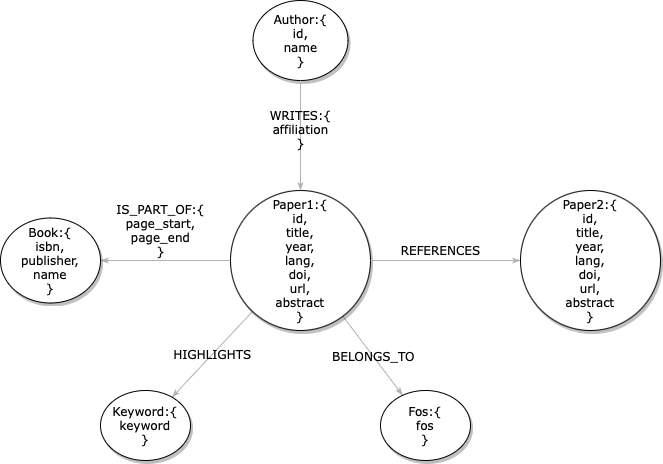
\includegraphics[width=0.9\textwidth]{Images/graph_diagram}
        \caption{Graph diagram of a Paper that references another one, it has a single Author, a Keyword, a Fos and it is part of a Book.}
        \label{fig:graph_diagram}%
    \end{center}
\end{figure}


\chapter{Commands and queries}
\label{ch:commands_and_queries_neo4j}%
The following commands and queries are written thinking principally on the way the database will be used.
We think a user with the necessity to upload or search for something in the system, will be able to do that with what we provide.
Longer and more difficult commands and queries can be written but we want to present only the ones that we find more meaningful.

We choose to use parameters instead of writing fixed values inside the queries to make the code as flexible as possible.
For this reason, the commands and queries can be also used changing the values of the parameters and obtaining the results of interest.
To execute the following code is required to run first the parameters regarding the command or query we want to perform and then the command or query itself.


\section{Commands}
\label{sec:commands}%
The following commands are provided to make possible the update of the data.
Each command can be easily modified to update parts of the database with specific features, for example, it is possible to use the queries of the next section to update the obtained nodes and their attributes.

\begin{enumerate}
    \item \textbf{Create a node, its attributes, and some relationships} \\
    The command creates a set of new nodes.
    In particular, the query aims to add a new paper to the database, whose author is already present within the system, and also set its properties.
    Here we add a new paper, set also its attributes, and create the nodes of the keywords and the fields of study of the paper if needed.
    The \verb|MERGE| command is what is used to create nodes and relationships checking also whether the new instances are already present within the database.
    This command allows us to avoid the creation of many copies of the same entity.
    The following command after adding the specified nodes creates also the relationships between them: the ones that relate the paper to its author, to its keywords, and to the specific study.

    \textbf{Parameters}
    \begin{lstlisting}[label={lst:parameters_command1neo4j}]
:param auth_id => "53f463b3dabfaee4dc8430d5";
:param auth_name => "Annabel Sebag";
:param affiliation => "53f463b3dabfaee4dc8430d5";

:param doi => "10.1145/1596685.1596829";
:param paper_id => "53e997cbb7602d9701fbcee3";
:param paper_title => "Yankee gal";
:param year => 2009;
:param lang => "en";
:param page_start => 155;
:param page_end => 155;
:param url => ["https://dx.doi.org/10.1145/1596685.1596829","https://doi.acm.org/10.1145/1596685.1596829","db/conf/siggraph/siggraph2009festival.html#Sebag09c","https://doi.org/10.1145/1596685.1596829"];
:param abstract => "This is a graduate film from the students of Supinfocom Valenciennes.";

:param k1 => "yankee gal";
:param k2 => "supinfocom valenciennes";
:param k3 => "graduatethe query aims"animation";
:param fos2 => "siggraph";
    \end{lstlisting}
    \textbf{Command}
    \begin{lstlisting}[label={lst:command1neo4j}]
MATCH (a:Author {id:$auth_id, name: $auth_name})
MERGE (new_p:Paper
        {doi:$doi,
        id:$paper_id,
        title:$paper_title,
        year:$year,
        lang:$lang,
        page_start:$page_start,
        page_end:$page_end,
        url:$url,
        abstract:$abstract})
MERGE aff = (a)-[:WRITES {affiliation:$affiliation}]->(new_p)
MERGE f1 = (new_p)-[:BELONGS_TO]->(:Fos {fos: $fos1})
MERGE f2 = (new_p)-[:BELONGS_TO]->(:Fos {fos: $fos2})
MERGE k1 = (new_p)-[:HIGHLIGHTS]->(kw1:Keyword {keyword:$k1})
MERGE k2 = (new_p)-[:HIGHLIGHTS]->(kw2:Keyword {keyword:$k2})
MERGE k3 = (new_p)-[:HIGHLIGHTS]->(kw3:Keyword {keyword:$k3})
RETURN aff, f1, f2, k1, k2, k3
    \end{lstlisting}
    \item \textbf{Create the relationship between existing nodes and set its properties} \\
    The command creates a new relationship between already existing nodes.
    In particular here is created the relationship which states that the author \verb|"James Ostell"| has written the paper titled \verb|"Grow"| when he was affiliated to organization \verb|"Federal| \verb|Institute of Technology, Switzerland"|.
    For better identification of the book and for avoiding linking all the books having the same title we could have used the identifier of the book instead of the title.
    We used \verb|MERGE| so if the relationship already exists with the specified affiliation it won't be added.

    \textbf{Parameters}
    \begin{lstlisting}[label={lst:parameters_command2neo4j}]
:param name => "James Ostell";
:param title => "Grow";
:param affiliation => "Federal Institute of Technology, Switzerland";
    \end{lstlisting}
    \textbf{Command}
    \begin{lstlisting}[label={lst:command2neo4j}]
MATCH (a:Author {name:$name}), (np:Paper {title:$title})
MERGE res = (a)-[:WRITES {affiliation:$affiliation}]->(np)
RETURN res;
    \end{lstlisting}
    \item \textbf{Set a new label for a node} \\
    We want to modify the properties of an already existing node.
    In particular, we want to add one label to a specific node.
    At first, we have new entries that are sparse data and we don’t know the exact type and source so we want to infer it, in particular, we check if they have the \verb|isbn| and in that case, we update the data, setting the nodes as books.
    We do this by controlling the papers and using the \verb|SET| keyword to update the properties, and if there are some misaligned data already in the graph this corrects that too.
    In the command, we can return the nodes in order to be sure that the information was updated correctly.
    We could do the same for the relationships, and we could also add more than one label.
    \begin{lstlisting}[label={lst:command3neo4j}]
MATCH (p:Publication)
WHERE p.isbn IS NOT NULL
SET p:Book
RETURN p;
    \end{lstlisting}
    \item \textbf{Update attributes of a relationship (analog for nodes)} \\
    The next command updates the values of the attributes of a specific relationship.
    In particular, the number of the starting and ending pages of the paper with id \verb|53e99785b7602d9701f40556| are set through the keyword \verb|SET|.
    If the user makes a mistake while inserting the properties of the relationship \verb|IS_PART_OF|, let's say the pages, the user can always modify afterwards the entries with the \verb|SET| operation.
    With the same syntax, if new properties come up or something was missed when adding nodes or relationships it is possible to create new attributes and set them to a specific value.

    \textbf{Parameters}
    \begin{lstlisting}[label={lst:parameters_command4neo4j}]
:param id => "53e99785b7602d9701f40556";
    \end{lstlisting}
    \textbf{Command}
    \begin{lstlisting}[label={lst:command4neo4j}]
MATCH (paper:Paper)-[i:IS_PART_OF]->(:Book)
WHERE paper.id = $id
SET i.page_start = 15
SET i.page_end = 33
    \end{lstlisting}
    \item \textbf{Remove attributes of a relationship (analogous for nodes)} \\
    The following commands remove some attributes from a relationship.
    In particular, we remove the attributes concerning the starting and ending numbers of pages within a book when these numbers are negative.
    We also remove these numbers when the index of the starting page is greater than the index of the ending page because it doesn't make sense to have such data.
    This can be seen as some sort of data cleaning, useful to remove incorrect data.
    \begin{lstlisting}[label={lst:command5neo4j1}]
MATCH (:Paper)-[i:IS_PART_OF]->(:Book)
WHERE i.page_start < 0
REMOVE i.page_start
    \end{lstlisting}
    \begin{lstlisting}[label={lst:command5neo4j2}]
MATCH (:Paper)-[i:IS_PART_OF]->(:Book)
WHERE i.page_end < 0
REMOVE i.page_end
    \end{lstlisting}
    \begin{lstlisting}[label={lst:command5neo4j3}]
MATCH (:Paper)-[i:IS_PART_OF]->(:Book)
WHERE NOT i.page_start IS NULL AND NOT i.page_end IS NULL AND i.page_end - i.page_start < 0
REMOVE i.page_start, i.page_end
    \end{lstlisting}
    \item \textbf{Delete a node} \\
    With the following command we delete the node \verb|Book| titled \verb|"Mathematics| \verb|and| \verb|Computers| \verb|in| \verb|Simulation"|, using the \verb|DELETE| keyword.
    Before performing the delete action, we use the \verb|DETACH| keyword that assures that all the relationships in which the node was involved are detached from the node itself in order to be able to remove it.

    \textbf{Parameters}
    \begin{lstlisting}[label={lst:parameters_command6neo4j}]
:param name => "Mathematics and Computers in Simulation";
    \end{lstlisting}
    \textbf{Command}
    \begin{lstlisting}[label={lst:command6neo4j}]
MATCH (b:Book {name:$name})
DETACH DELETE b;
    \end{lstlisting}
\end{enumerate}


\section{Queries}
\label{sec:queries}%
\begin{enumerate}
    \item \textbf{Authors who wrote a certain paper} \\
    The query returns a graph with all the authors who wrote the papers titled \verb|"CodeTalk"|.
    This is a very simple query that can be very useful in everyday searches.

    \textbf{Parameters}
    \begin{lstlisting}[label={lst:parameters_query1neo4j}]
:param title => "CodeTalk";
    \end{lstlisting}
    \textbf{Query}
    \begin{lstlisting}[label={lst:query1neo4j}]
MATCH g = (:Author)-[:WRITES]->(:Paper {title:$title})
RETURN g
    \end{lstlisting}
    \begin{figure}[H]
        \begin{center}
            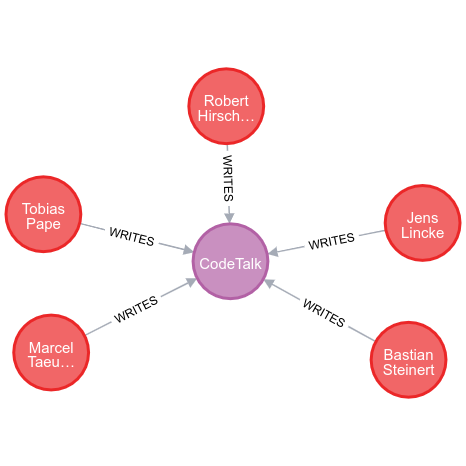
\includegraphics[trim={0 1cm 0 0}, clip, width=0.45\textwidth]{Images/query1neo4j}
            \label{fig:query1neo4j}%
        \end{center}
    \end{figure}
    \item \textbf{Previous affiliations of an author} \\
    The query returns all the organizations to whom the author \verb|"Annabel Sebag"| has been affiliated sorted by the year in which she wrote the paper with that affiliation.

    \textbf{Parameters}
    \begin{lstlisting}[label={lst:parameters_query2neo4j}]
:param name => "Annabel Sebag";
    \end{lstlisting}
    \textbf{Query}
    \begin{lstlisting}[label={lst:query2neo4j}]
MATCH (:Author {name:$name})-[r:WRITES]-(p:Paper)
WITH r.affiliation AS affiliation, p.year AS year
ORDER BY year DESC
RETURN DISTINCT affiliation, year
    \end{lstlisting}
    \begin{figure}[H]
        \begin{center}
            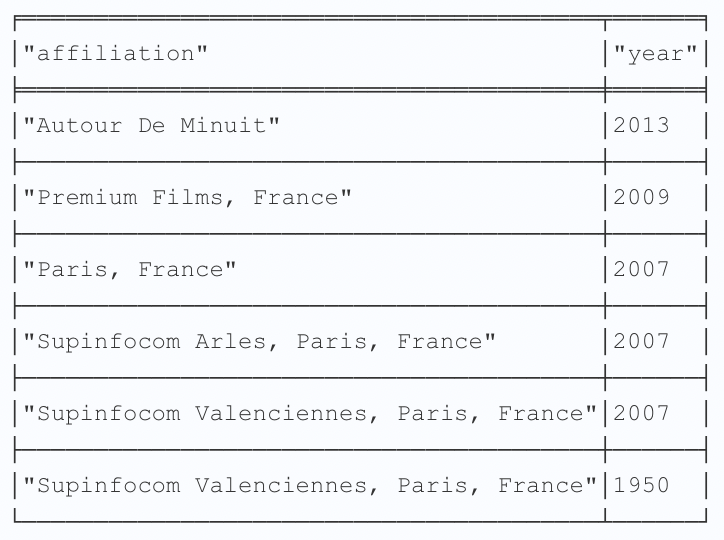
\includegraphics[width=0.45\linewidth]{Images/query2neo4j}
            \label{fig:query2neo4j}%
        \end{center}
    \end{figure}
    \item \textbf{Authors who wrote for a journal in a specific year} \\
    The query returns all the authors who wrote at least a paper for the journal named \verb|"Briefings in Bioinformatics"| in the year \verb|2005|.
    In the return statement we use the keyword \verb|DISTINCT| in order to count only once each author because we only want to know if the author wrote on that paper in the specified year, and not how many times.

    \textbf{Parameters}
    \begin{lstlisting}[label={lst:parameters_query3neo4j}]
:param name => "Briefings in Bioinformatics";
:param year => 2005;
    \end{lstlisting}
    \textbf{Query}
    \begin{lstlisting}[label={lst:query3neo4j}]
MATCH (a:Author)-[:WRITES]->(p:Paper)-[:IS_PART_OF]->(j:Journal)
WHERE p.year = $year AND j.name = $name
RETURN DISTINCT a.name AS authorName
    \end{lstlisting}
    \begin{figure}[H]
        \begin{center}
            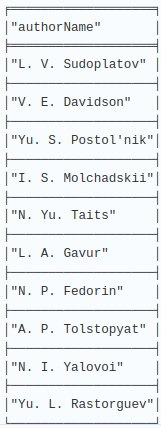
\includegraphics[width=0.45\textwidth]{Images/query3neo4j}
            \label{fig:query3neo4j}%
        \end{center}
    \end{figure}
    \item \textbf{Papers that belong to a Journal, written by authors while they were affiliated to a certain organization} \\
    The query returns the names of all the journals written by authors while they were affiliated with the organization named \verb|"Wien"|.

    In some of the queries we have seen before, we retrieved from the database the affiliations related to the authors.
    It is also interesting to see how easily we can retrieve the authors that are related to a certain affiliation, and then explore the relationships of the author in order to obtain meaningful data, useful for everyday search in the bibliography database.
    The next query is very fast because centered mostly on relationships, a natural characteristic of graphs.

    \textbf{Parameters}
    \begin{lstlisting}[label={lst:parameters_query4neo4j}]
:param affiliation => "Wien";
    \end{lstlisting}
    \textbf{Query}
    \begin{lstlisting}[label={lst:query4neo4j}]
MATCH (:Author)-[:WRITES {affiliation:$affiliation}]->(:Paper)-[:IS_PART_OF]->(b:Journal)
RETURN DISTINCT b.name as journalName;
    \end{lstlisting}
    \begin{figure}[H]
        \begin{center}
            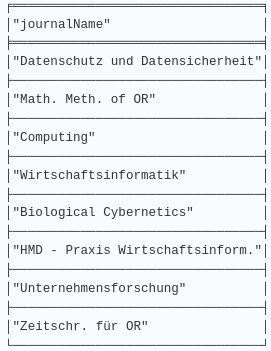
\includegraphics[width=0.45\textwidth]{Images/query4neo4j}
            \label{fig:query4neo4j}%
        \end{center}
    \end{figure}
    \item \textbf{Authors which published more papers in journals in a specific year} \\
    The query returns the five authors that published more papers in the year \verb|2000| in journals sorted by the number of papers they published.
    We use the function \verb|count()| to obtain for each author the relative number of papers and limit the output to the first five authors discovered during the search.

    \textbf{Parameters}
    \begin{lstlisting}[label={lst:parameters_query5neo4j}]
:param year => 2000;
    \end{lstlisting}
    \textbf{Query}
    \begin{lstlisting}[label={lst:query5neo4j}]
MATCH (a:Author)-[:WRITES]->(p:Paper)-[:IS_PART_OF]->(:Journal)
WHERE p.year = $year
WITH a, count(*) AS paperNum
RETURN a.name AS authorName, paperNum
ORDER BY paperNum DESC LIMIT 5;
    \end{lstlisting}
    \begin{figure}[H]
        \begin{center}
            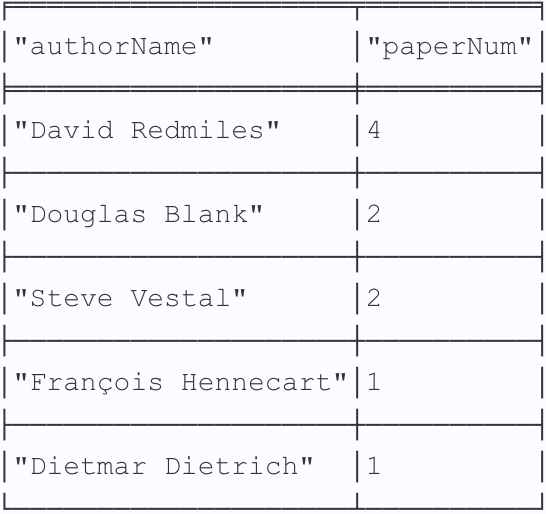
\includegraphics[width=0.45\textwidth]{Images/query5neo4j}
            \label{fig:query5neo4j}%
        \end{center}
    \end{figure}
    \item \textbf{Number of papers written in conferences by authors whose name starts with specific letters per venue} \\
    The query returns for each venue the number of papers that have been presented in a conference considering only papers that are written by authors whose name starts for \verb|"A"| or \verb|"S"|.

    \textbf{Parameters}
    \begin{lstlisting}[label={lst:parameters_query6neo4j}]
:param letter1 => "A";
:param letter2 => "S";
    \end{lstlisting}
    \textbf{Query}
    \begin{lstlisting}[label={lst:query6neo4j}]
MATCH (a:Author)-[:WRITES]->(p:Paper)-[:IS_PART_OF]->(c:Conference)
WHERE a.name STARTS WITH $letter1 OR a.name STARTS WITH $letter2
WITH c.name AS conference, c.location AS location,
     count(DISTINCT p) AS number_of_papers
RETURN DISTINCT conference, location, number_of_papers
ORDER BY number_of_papers DESC LIMIT 5;
    \end{lstlisting}
    \begin{figure}[H]
        \begin{center}
            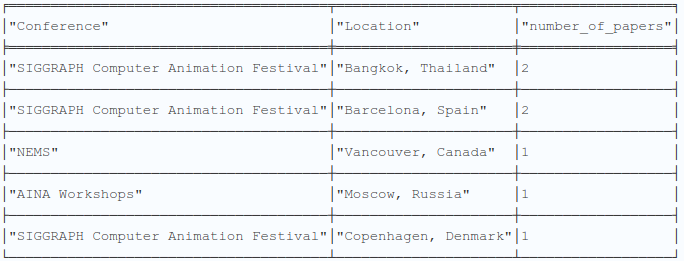
\includegraphics[width=0.9\textwidth]{Images/query6neo4j}
            \label{fig:query6neo4j}%
        \end{center}
    \end{figure}
    \item \textbf{Authors who wrote the most referenced papers which belong to publications of type book, while they were affiliated to a specific organization} \\
    The query returns the authors whose papers have been referenced the most in papers that are part of books while they were affiliated to \verb|"University of Mannheim"|.
    We also want to retrieve only authors that published at least 2 papers, so we filter furthermore the result.

    \textbf{Parameters}
    \begin{lstlisting}[label={lst:parameters_query7neo4j}]
:param affiliation => "University of Mannheim";
    \end{lstlisting}
    \textbf{Query}
    \begin{lstlisting}[label={lst:query7neo4j}]
MATCH (a:Author)-[w:WRITES]->(:Paper)<-[r:REFERENCES]-(:Paper)-[:IS_PART_OF]->(:Book)
WHERE w.affiliation = $affiliation
WITH a, count(DISTINCT r) AS totalReferences
WHERE totalReferences > 2
RETURN a.name AS authorName, totalReferences;
    \end{lstlisting}
    \begin{figure}[H]
        \begin{center}
            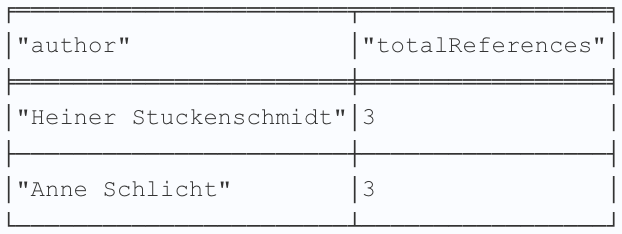
\includegraphics[width=0.45\linewidth]{Images/query7neo4j}
            \label{fig:query7neo4j}%
        \end{center}
    \end{figure}
    \item \textbf{Papers indirectly referenced by other papers at a certain distance of steps} \\
    The query returns different papers linked to each other by the relation \verb|REFERENCES| at a distance of steps between 3 and 6.
    We limit the results in order to get the output as soon as the process finds 5 rows that respect the filter of the search.
    \begin{lstlisting}[label={lst:query8neo4j1}]
MATCH (a1:Paper), (a2:Paper)
WHERE id(a1) <> id(a2) AND (EXISTS {MATCH (a1)-[:REFERENCES*3..6]->(a2)})
RETURN DISTINCT a1.title AS firstPaper, a2.title AS secondPaper
LIMIT 5;
    \end{lstlisting}
    \begin{figure}[H]
        \begin{center}
            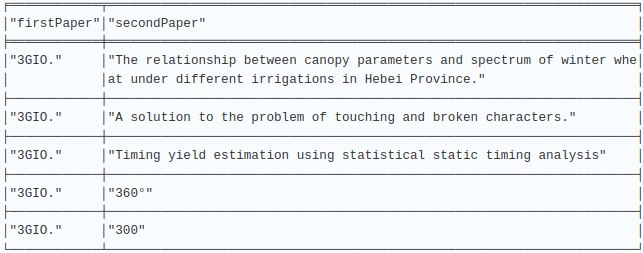
\includegraphics[width=0.9\textwidth]{Images/query8neo4j1}
            \label{fig:query8neo4j}%
        \end{center}
    \end{figure}
    The performance is not optimal and using the \verb|PROFILE| command in the same query we can see how the search is actually made in the graph using this specific interrogation on the database.
    \begin{lstlisting}[label={lst:profile_query8neo4j1}]
PROFILE
MATCH (a1:Paper), (a2:Paper)
WHERE id(a1) <> id(a2) AND (EXISTS {MATCH (a1)-[:REFERENCES*3..6]->(a2)})
RETURN DISTINCT a1.title AS firstPaper, a2.title AS secondPaper LIMIT 5;
    \end{lstlisting}
    \begin{figure}[H]
        \begin{center}
            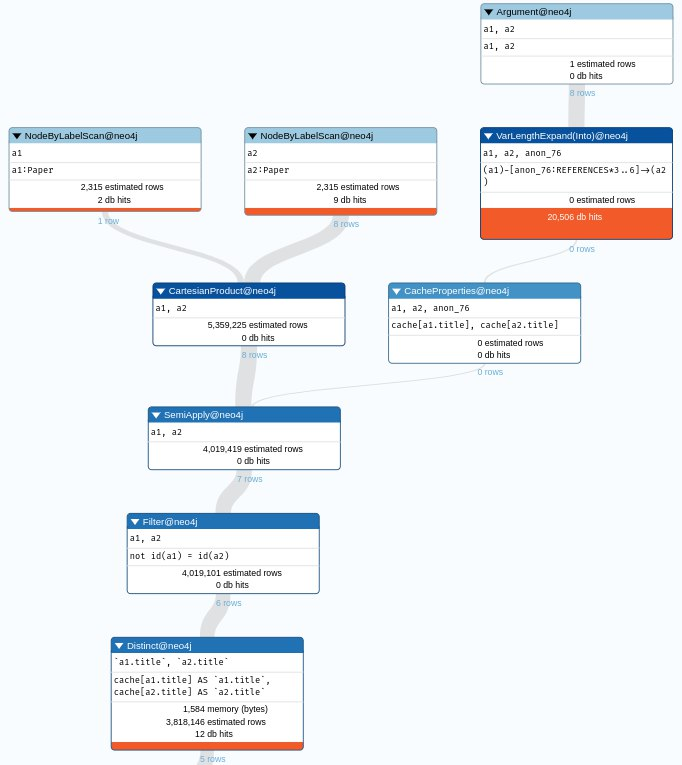
\includegraphics[width=0.9\textwidth]{Images/profile_query8neo4j1}
            \label{fig:profile_query8neo4j1}%
        \end{center}
    \end{figure}
    We can notice that the execution of the query is done in parallel trying on one side to perform the \verb|MATCH| of the two papers separately and on the other side to find the relationships between the two papers given by \verb|REFERENCES| from 3 to 6 steps away.
    The two results of the search are then merged together. \\
    In this process, we estimated a lot of rows and wasted time, by doing the controls individually.
    \begin{figure}[H]
        \begin{center}
            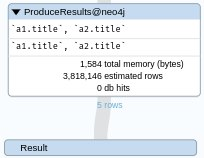
\includegraphics[width=0.45\textwidth]{Images/result_query8neo4j1}
            \label{fig:result_query8neo4j1}%
        \end{center}
    \end{figure}
    To make the query more efficient we can bring the filtering of the data a step ahead, so we can check directly in the \verb|MATCH| command for the relationships between the papers.
    \begin{lstlisting}[label={lst:query8neo4j2}]
MATCH (a1:Paper)-[:REFERENCES*3..6]->(a2:Paper)
WHERE id(a1) <> id(a2)
RETURN DISTINCT a1.title AS firstPaper, a2.title AS secondPaper
LIMIT 5;
    \end{lstlisting}
    We notice that the results can be different from the precedent approach, due to the use of \verb|LIMIT| that stops the research as soon as it gets the 5 results of interest and in this case, the search is done differently so the outputs are not the same.
    \begin{figure}[H]
        \begin{center}
            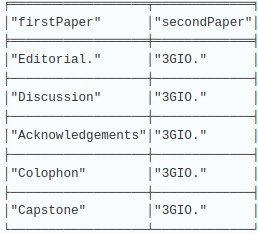
\includegraphics[width=0.45\textwidth]{Images/query8neo4j2}
            \label{fig:query8neo4j2}%
        \end{center}
    \end{figure}
    Using this version of the query, we have that the search is more linear because, in \verb|MATCH|, we don't look for the papers separately but once matched a \verb|Paper| we search for its recursive \verb|REFERENCES| relationships and match at once the two papers and their connections.
    This approach is fast and improves efficiency.
    \begin{figure}[H]
        \begin{center}
            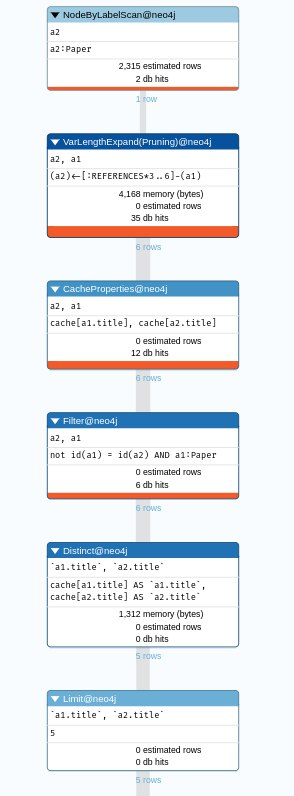
\includegraphics[width=0.45\textwidth]{Images/profile_query8neo4j2}
            \label{fig:profile_query8neo4j2}%
        \end{center}
    \end{figure}
    We can see that reaching the result the command required more memory, but we didn't estimate useless rows of data, extracting only what we are interested in without an extended search on the graph.
    \begin{figure}[H]
        \begin{center}
            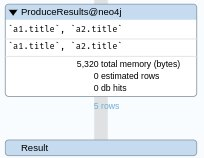
\includegraphics[width=0.45\textwidth]{Images/result_query8neo4j2}
            \label{fig:result_query8neo4j2}%
        \end{center}
    \end{figure}
    Alternatively, we can tackle this search from another point of view.
    We can use a query based precisely on the steps we are interested in, making the query more explicit and getting other results, because in the recursive form the process could stop before reaching this exact amount of steps, especially using the \verb|LIMIT| keyword.
    \begin{lstlisting}[label={lst:query8neo4j3}]
MATCH (a1:Paper)-[:REFERENCES]->(a2:Paper)-[:REFERENCES]->(a3:Paper)-[:REFERENCES]->(a4:Paper)-[:REFERENCES]->(a5:Paper)-[:REFERENCES]->(a6:Paper)
WHERE id(a1) <> id(a2) AND id(a2) <> id(a3) AND id(a3) <> id(a4) AND id(a4) <> id(a5) AND id(a5) <> id(a6)
RETURN DISTINCT a1.title AS firstPaper, a6.title AS secondPaper
LIMIT 5;
    \end{lstlisting}
    \begin{figure}[H]
        \begin{center}
            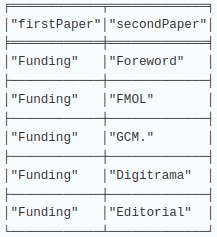
\includegraphics[width=0.45\textwidth]{Images/query8neo4j3}
            \label{fig:query8neo4j3}%
        \end{center}
    \end{figure}
    \item \textbf{Best collaborator of all times for each author in terms of papers written in journals} \\
    The following query allows the researcher to understand each author who is the best collaborator of all time considering their collaborations in journals.
    In the result, we can sometimes see symmetry in the data, if an author has another as the best collaborator and vice versa.

    Firstly we do a \verb|MATCH| imposing our constraints.
    Secondly, we group by authors and co-authors counting for each couple how many papers were published in journals they wrote together, and we order the table by this number in descending order.
    On the next \verb|WITH| clause for each author we extract only the best collaborator, namely the one with whom he wrote more papers in journals.

    \textbf{Query}
    \begin{lstlisting}[label={lst:query9neo4j}]
MATCH (a:Author)-[:WRITES]->(p:Paper)<-[:WRITES]-(ca:Author), (p)-[:IS_PART_OF]->(:Journal)
WITH DISTINCT a, ca, count(DISTINCT p) AS cnt ORDER BY cnt DESC
WITH DISTINCT a, collect(ca.name) AS colabs, collect(cnt) AS cnts
RETURN a.name AS author, colabs[0] AS bestCollaborator, cnts[0] AS numberOfPapers LIMIT 5
    \end{lstlisting}
    \begin{figure}[H]
        \begin{center}
            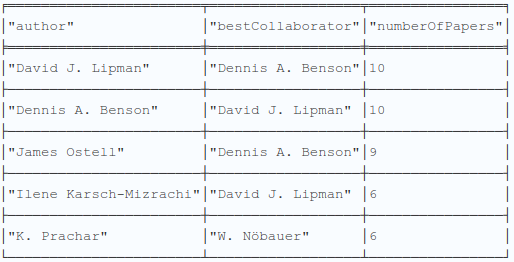
\includegraphics[width=0.9\textwidth]{Images/query9neo4j}
            \label{fig:query9neo4j}%
        \end{center}
    \end{figure}
    \item \textbf{Papers which are at the base of a given field of study} \\
    The query returns the papers which are at the base of a given field of study.
    To be the base for a field of study means to not reference directly or indirectly other papers of that field of study.
    With this query, we retrieve the papers that are probably at the base of some field of study because an upper bound of 7 is chosen to check the indirect references. \\
    A variant of this query can be to retrieve the authors who wrote the base papers of a field of study, so the authors are the ``founders'' of that field.
    The query is more meaningful if run on a very large set of data.
    \textbf{Parameters}
    \begin{lstlisting}[label={lst:parameters_query10neo4j}]
:param fos => "Statistics";
    \end{lstlisting}
    \textbf{Query}
    \begin{lstlisting}[label={lst:query10neo4j}]
MATCH (founder:Paper)-[:BELONGS_TO]->(fos:Fos{fos:$fos})<-[:BELONGS_TO]-(p:Paper)
WHERE id(founder) <> id(p)
WITH collect(p) AS test, founder, fos
WHERE all(p IN test WHERE NOT EXISTS((founder)-[:REFERENCES*7]->(p)))
RETURN fos AS field, collect(DISTINCT founder.title) AS founderPapers
    \end{lstlisting}
    \begin{figure}[H]
        \begin{center}
            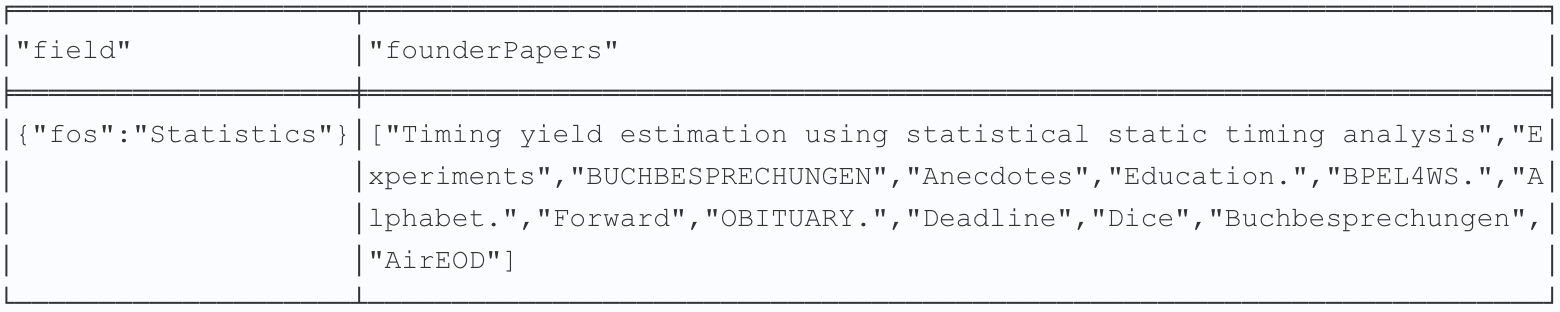
\includegraphics[width=0.9\linewidth]{Images/query10neo4j}
            \label{fig:query10neo4j}%
        \end{center}
    \end{figure}
    \item \textbf{Total pages written by the authors of an organization within a journal} \\
    The query returns the total number of pages written by authors affiliated with the organization \verb|"Federal Institute of Technology, Switzerland"| within journals.
    The function \verb|avg()| can be used to compute the average of the pages written by an author in the papers.

    \textbf{Parameters}
    \begin{lstlisting}[label={lst:parameters_query11neo4j}]
:param affiliation=>"Federal Institute of Technology, Switzerland";
    \end{lstlisting}
    \textbf{Query}
    \begin{lstlisting}[label={lst:query11neo4j}]
MATCH (a:Author)-[w:WRITES {affiliation:$affiliation}]->(p:Paper)-[i:IS_PART_OF]->(j:Journal)
WHERE i.page_start IS NOT NULL AND i.page_end IS NOT NULL
WITH a, sum(i.page_end - i.page_start) AS num_pag
ORDER BY num_pag DESC
RETURN a AS Author, num_pag;
    \end{lstlisting}
    \begin{figure}[H]
        \begin{center}
            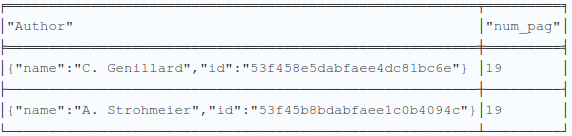
\includegraphics[width=0.9\textwidth]{Images/query11neo4j}
            \label{fig:query11neo4j}%
        \end{center}
    \end{figure}
    \item \textbf{Organizations which have published their own more papers within a specific journal with associated fields of study} \\
    The query returns the organizations which have exclusively written more papers, which means that the authors of the papers have all the same affiliation on \verb|"Commun . ACM"|.
    The query provides the fields of study on which the considered papers were focused on.

    \textbf{Parameters}
    \begin{lstlisting}[label={lst:parameters_query12neo4j}]
:param journalTitle => "Commun. ACM";
    \end{lstlisting}
    \textbf{Query}
    \begin{lstlisting}[label={lst:query12neo4j}]
MATCH (a1:Author)-[w1:WRITES]->(p1:Paper)-[:IS_PART_OF]->(j:Journal {name:$journalTitle}), (p1:Paper)-[:BELONGS_TO]->(fos:Fos), (a2:Author)-[w2:WRITES]-(p1:Paper)
WHERE a1 <> a2 AND w1.affiliation IS NOT NULL
WITH w1.affiliation AS affiliation, collect(DISTINCT fos) AS fieldsOfStudy, collect(DISTINCT w2.affiliation) AS others, count(DISTINCT p1) AS numberOfPapers
WHERE ALL(organization IN others WHERE affiliation=organization)
WITH affiliation, fieldsOfStudy, numberOfPapers
ORDER BY numberOfPapers DESC
RETURN affiliation, fieldsOfStudy, numberOfPapers
LIMIT 2
    \end{lstlisting}
    \begin{figure}[H]
        \begin{center}
            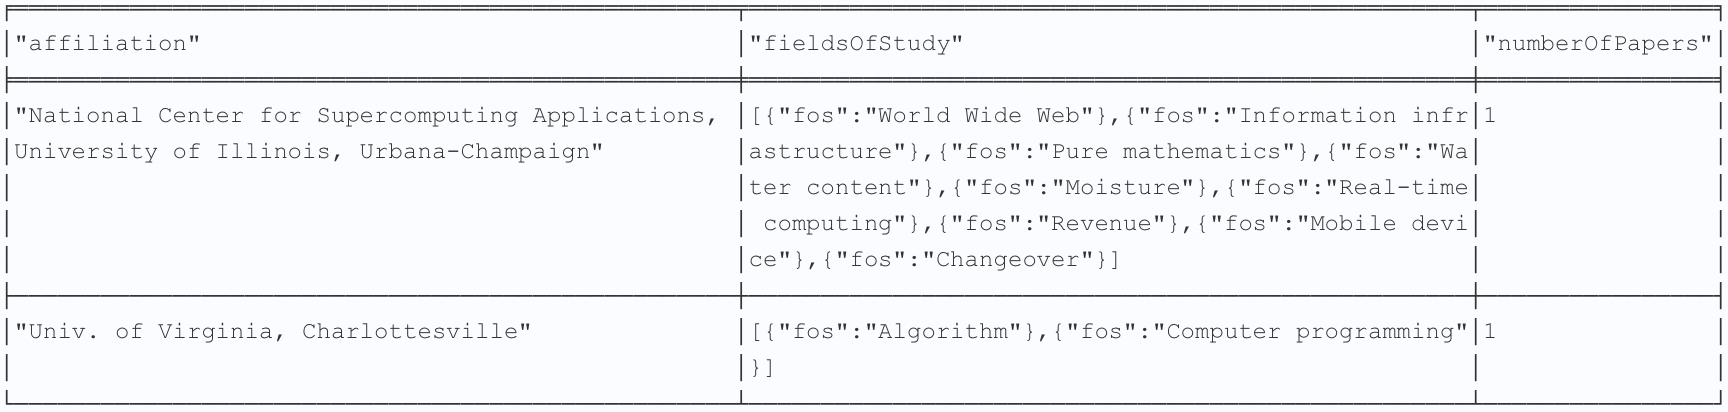
\includegraphics[width=0.9\linewidth]{Images/query12neo4j}
            \label{fig:query12neo4j}%
        \end{center}
    \end{figure}
    \item \textbf{Recommended books given one book} \\
    The query returns the book considered the nearest to the one given as a parameter.
    The similarity between books is evaluated in terms of the number of keywords associated with the papers linked to the books.
    In addition, fields of study which are common to the two books are shown.
    \begin{lstlisting}[label={lst:parameters_query13neo4j}]
:param title => "RoboCup 2009";
    \end{lstlisting}
    \textbf{Query}
    \begin{lstlisting}[label={lst:query13neo4j}]
MATCH (p1:Paper)-[:IS_PART_OF]->(b1:Book),
(p1:Paper)-[:BELONGS_TO]->(fos1:Fos)<-[:BELONGS_TO]-(p2:Paper),
(p1)-[:HIGHLIGHTS]->(k1:Keyword)<-[:HIGHLIGHTS]-(p2),
(p2:Paper)-[:IS_PART_OF]->(b2:Book)
WHERE b1 <> b2 AND p1 <> p2 AND b1.name = $title
WITH b1, b2, collect(DISTINCT fos1) AS fos, count(DISTINCT k1) AS score
ORDER BY score DESC
RETURN b2.name AS relatedBook, fos, score
LIMIT 3;
    \end{lstlisting}
    \begin{figure}[H]
        \begin{center}
            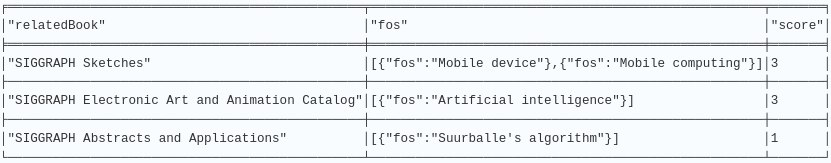
\includegraphics[width=0.9\textwidth]{Images/query13neo4j}
            \label{fig:query13neo4j}%
        \end{center}
    \end{figure}
    \item \textbf{Possible new interesting collaborations between authors in the same fields of study} \\
    The query returns the new possible interesting collaborations, by which we mean the couple of authors who haven't written a paper together but have written many times with common authors and wrote about similar topics, so they are involved in the same fields of study.

    \textbf{Parameters}
    \begin{lstlisting}[label={lst:parameters_query14neo4j}]
:param minimum_collabs =>1;
    \end{lstlisting}
    \textbf{Query}
    \begin{lstlisting}[label={lst:query14neo4j}]
MATCH
(a1:Author)-[w1:WRITES]->(p1:Paper)<-[w2:WRITES]-(a2:Author),
(a2:Author)-[w3:WRITES]->(p2:Paper)<-[w4:WRITES]-(a3:Author),
(a1)-[:WRITES]->(p3:Paper)-[:BELONGS_TO]->(f1:Fos)<-[:BELONGS_TO]-(p4:Paper)<-[:WRITES]-(a3)
WHERE NOT EXISTS ((a1)-[:WRITES]->(:Paper)<-[:WRITES]-(a3)) AND a1 <> a3 AND a1 <> a2 AND a2 <> a3
WITH a1, a3, collect(DISTINCT f1.fos) AS fields, count(DISTINCT f1) AS common_fields, count(DISTINCT p1) AS common_collabs1, count(DISTINCT p2) AS common_collabs2
WHERE common_collabs1 > $minimum_collabs AND common_collabs2 > $minimum_collabs
WITH a1, a3, fields, common_fields, common_collabs1 + common_collabs2 AS common_collabs
ORDER BY common_fields DESC, common_collabs DESC
RETURN DISTINCT a1.name as Author1, a3.name as Author2, fields, common_collabs, common_fields
LIMIT 5
    \end{lstlisting}
    \begin{figure}[H]
        \begin{center}
            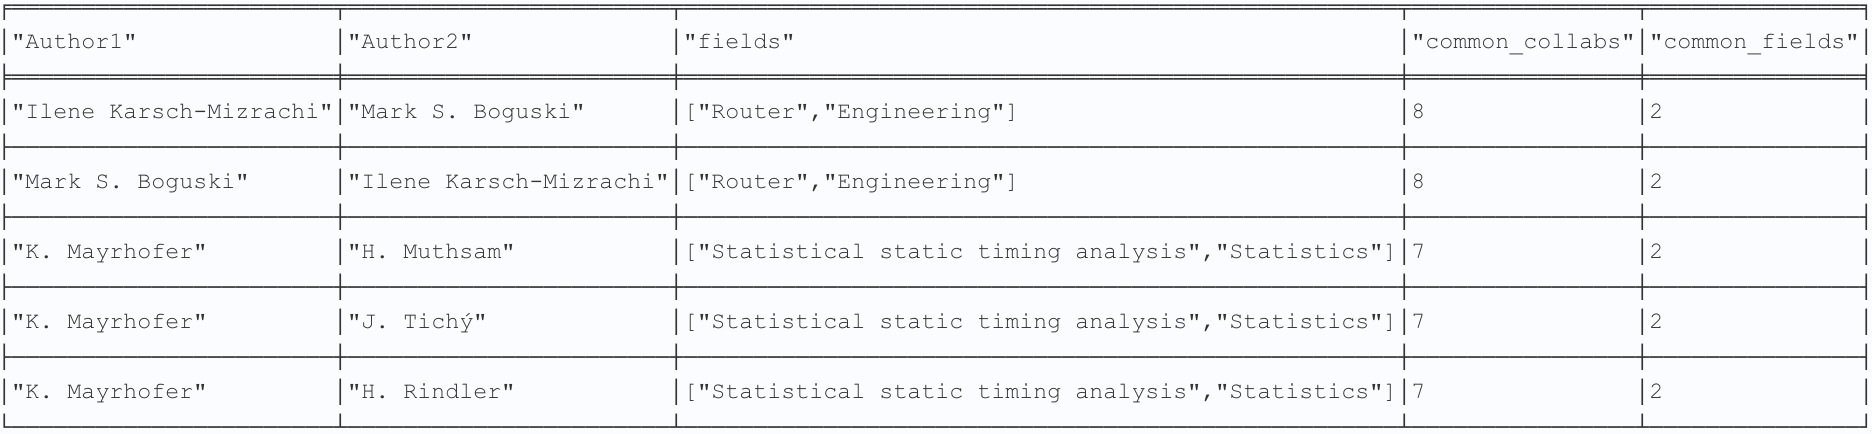
\includegraphics[width=0.9\textwidth]{Images/query14neo4j}
            \label{fig:query14neo4j}%
        \end{center}
    \end{figure}
    \item \textbf{Shortest connection between two papers with no common field of study} \\
    With this query, we want to find what is the shortest path, by navigating the references, between two papers that do not have any field of study in common.
    Firstly we bound the papers node and the associated field of studies to variables \verb|p1/p2| and \verb|fos1/fos2| respectively and we impose that \verb|p1| and \verb|p2| must be different.
    Secondly, we collect the fields of study associated with each paper and put a condition stating that the intersection of these two collection must be zero.
    Finally, we call the \verb|shortestPath| function and impose all the conditions on the path to be found;
    we put an upper bound of 7 to the length of the path to avoid searching too deep in the graph and limited the search to the first valid path found using the clause \verb|WITH sp LIMIT 1|, where \verb|sp| refers to the result of the call to the \verb|shortestPath| function.

    \textbf{Parameters}
    \begin{lstlisting}[label={lst:parameters_query15neo4j}]
:param fos1 => "Irrigation";
:param fos2 => "Artificial intelligence";
    \end{lstlisting}
    \textbf{Query}
    \begin{lstlisting}[label={lst:query15neo4j}]
MATCH (fos1:Fos) <-[:BELONGS_TO]- (p1:Paper) -[:BELONGS_TO]-> (:Fos {fos:$fos1}),
      (fos2:Fos) <-[:BELONGS_TO]- (p2:Paper) -[:BELONGS_TO]-> (:Fos {fos:$fos2})
WHERE p1 <> p2
WITH p1, collect(DISTINCT fos1) AS foss1, p2, collect(DISTINCT fos2) AS foss2
WHERE all(f IN foss1 WHERE NOT f IN foss2)
MATCH sp = shortestPath((p1)-[:REFERENCES*..7]->(p2))
WHERE length(sp) > 1
RETURN sp LIMIT 1;
    \end{lstlisting}
    Below we can see the result of the query run with the aforementioned parameters.
    \begin{figure}[H]
        \begin{center}
            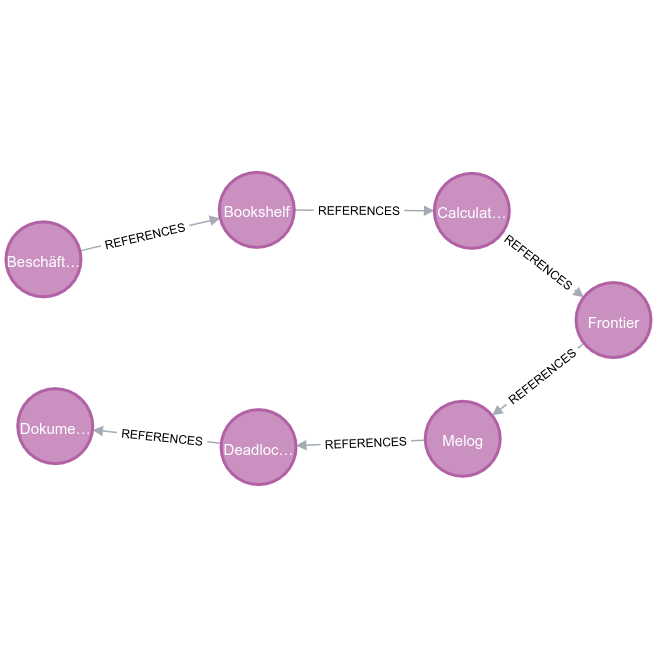
\includegraphics[trim={0 6cm 0 6cm}, clip, width=0.9\textwidth]{Images/query15neo4j}
            \label{fig:query15neo4j}%
        \end{center}
    \end{figure}
\end{enumerate}



    \part{MongoDB}
    \label{part:mongodb}%
    \chapter{Introduction to the problem}
\label{ch:introduction_to_the_problem_mongodb}%
In this part, we implement a bibliographic database through MongoDB, which is a document-oriented database.
In the previous part, using Neo4j, the main focus was on the relationships between nodes, instead, MongoDB's paradigm is different.
It shifts the attention to the document itself, which is the atomic and fundamental element of the database.
In this case, each document represents a single paper and contains all the related information.
All the articles are stored in the same collection called \verb|bibliography|.
A bibliographic database is a use case where the documental approach may be very successful.
The main focus of this kind of database is to store the information regarding every single paper without the need to relate many articles together and without doing very complex queries.


\chapter{Document structure}
\label{ch:document_structure_mongodb}%
Since we are using a documental database, papers are the main entity and, because of this, it is reasonable to store the text and the structure of the articles.
These fields are added to the attributes listed in the previous part regarding graph databases.
In particular, each paper is composed of many sections and each section has a title, several paragraphs, and a certain number of image URLs with associated captions.
Moreover, each section can contain subsections that have the same structure as a section.

In addition, also the email and bio of the authors have been added as well as the publication date of the article.

The following table shows the document's fields associated with their respective MongoDB type and meaning.
\begin{table}[H]
    \centering
    \begin{tabular}{| c | c | c |}
        \hline % \rowcolor{bluepoli!40}
        \textbf{Field name}      & \textbf{Type}   & \textbf{Description} \T\B \\
        \hline \hline
        \_id                     & String          & paper ID\T\B              \\
        title                    & String          & paper title\T\B           \\
        authors                  & Array of Object & list of authors\T\B       \\
        authors.\_id             & String          & author ID\T\B             \\
        authors.name             & String          & author name\T\B           \\
        authors.org              & String          & author affiliation\T\B    \\
        authors.email            & String          & author email\T\B          \\
        authors.bio              & String          & author short bio\T\B      \\
        keywords                 & Array of String & paper keywords\T\B        \\
        fos                      & Array of String & paper fields of study\T\B \\
        publication\_type        & String          & paper type\T\B            \\
        venue                    & String          & publication name\T\B      \\
        volume                   & Int32           & journal volume\T\B        \\
        issue                    & Int32           & journal issue\T\B         \\
        page\_start              & Int32           & start page\T\B            \\
        page\_end                & Int32           & end page\T\B              \\
        date                     & Date            & publication date\T\B      \\
        lang                     & String          & paper language\T\B        \\
        isbn                     & String          & book ISBN\T\B             \\
        issn                     & String          & journal ISSN\T\B          \\
        doi                      & String          & paper DOI\T\B             \\
        publisher                & String          & publisher name\T\B        \\
        location                 & String          & conference location\T\B   \\
        abstract                 & String          & paper abstract\T\B        \\
        url                      & Array of String & paper URLs\T\B            \\
        references               & Array of String & paper references\T\B      \\
        sections                 & Array of Object & paper sections\T\B        \\
        sections.title           & String          & section title\T\B         \\
        sections.paragraphs      & Array of String & section paragraphs\T\B    \\
        sections.subsections     & Array of Object & section subsections\T\B   \\
        sections.figures         & Array of Object & section figures\T\B       \\
        sections.figures.URL     & String          & figure URL\T\B            \\
        sections.figures.caption & String          & figure caption\T\B        \\
        \hline
    \end{tabular}
    \\[8pt]
    \caption{Description of the fields with related type and meaning.}
    \label{tab:document_structure_mongodb}%
\end{table}
Notes:
\begin{itemize}
    \item \verb|publication_type| can only assume ``Journal'', ``Book'' or ``Conference'' as value;
    \item a paper of type ``Journal'' can have the fields \verb|issn|, \verb|volume|, \verb|issue| and \verb|publisher|;
    \item a paper of type ``Book'' can have the fields \verb|isbn| and \verb|publisher|;
    \item a paper of type ``Conference'' can have the field \verb|location|;
    \item \verb|subsections| have the same structure as \verb|sections|, so they could contain multiple \verb|subsections| and so on in a recursively way.
    We decided to consider only one level of subsections, so \verb|subsections| don't have the \verb|subsections| field.
\end{itemize}
The following code snippet shows our document structure represented in JSON format.
\begin{lstlisting}[label={lst:document_structure_mongodb}]
{
    "_id": <String>,
    "title": <String>,
    "authors": [
        {
            "_id": <String>,
            "name": <String>,
            "email": <String>,
            "bio": <String>,
            "org": <String>
        }
    ],
    "abstract": <String>,
    "keywords": [<String>],
    "fos": [<String>],
    "publication_type": <String>,
    "venue": <String>,
    "volume": <Int32>,
    "issue": <Int32>,
    "issn": <String>,
    "publisher": <String>,
    "isbn": <String>,
    "location": <String>,
    "date": <ISODate>,
    "page_start": <Int32>,
    "page_end": <Int32>,
    "lang": <String>,
    "doi": <String>,
    "url": [<String>],
    "references": [<String>],
    "sections": [
        {
            "title": <String>,
            "paragraphs": [<String>],
            "figures": [
                {
                    "URL": <String>,
                    "caption": <String>
                }
            ],
            "subsections": [
                {
                  "title": <String>,
                  "paragraphs": [<String>],
                  "figures": [
                      {
                          "URL": <String>,
                          "caption": <String>
                      }
                  ]
                }
            ]
        }
    ]
}
\end{lstlisting}
Below we provide some examples of the three main paper types that appear in our document with their associated attributes.
The difference in the attributes is minimal and, as mentioned beforehand, it concerns the fields related to the publishing type of the paper.

\paragraph{Model of journal:}
This is the document structure for the papers published in journals.
\begin{figure}[H]
    \begin{center}
        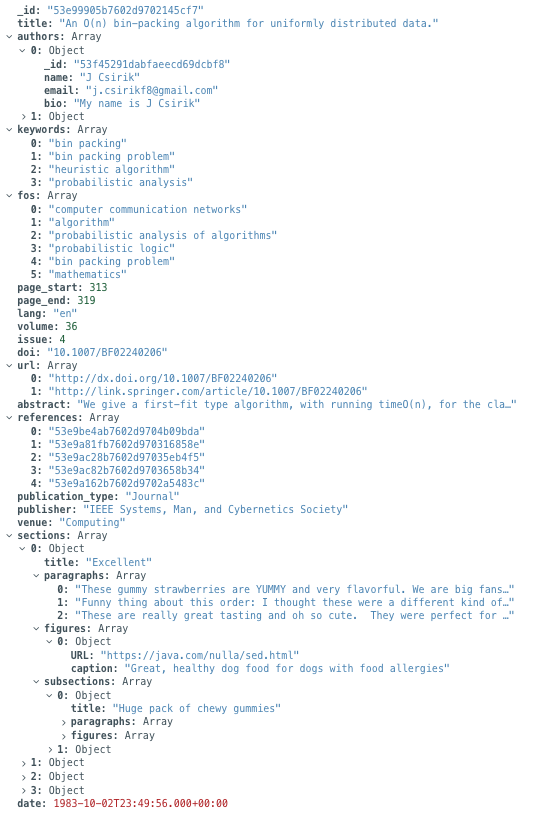
\includegraphics[width=0.9\linewidth]{ImagesMongoDB/journal}
        \label{fig:journal}%
    \end{center}
\end{figure}

\paragraph{Model of book:}
This is the document structure for the papers published in books.
\begin{figure}[H]
    \begin{center}
        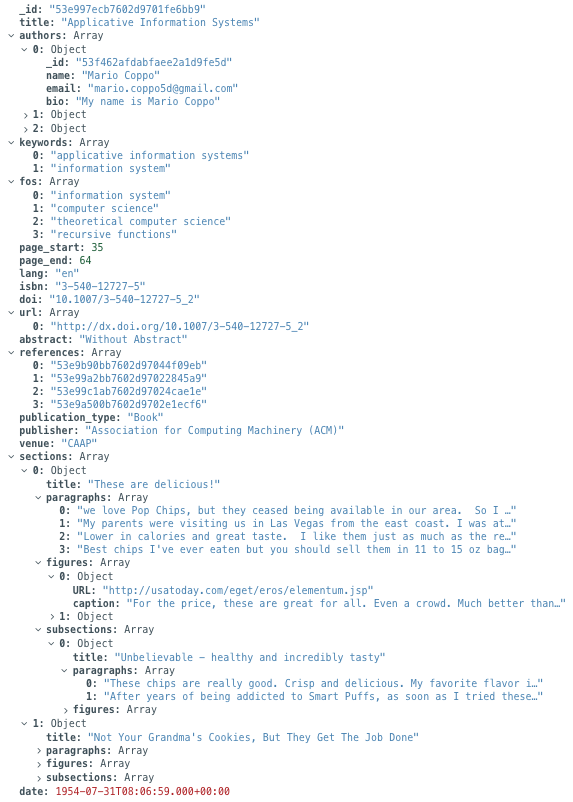
\includegraphics[width=0.9\linewidth]{ImagesMongoDB/book}
        \label{fig:book}%
    \end{center}
\end{figure}

\paragraph{Model of conference:}
This is the document structure for the papers published at conferences.
\begin{figure}[H]
    \begin{center}
        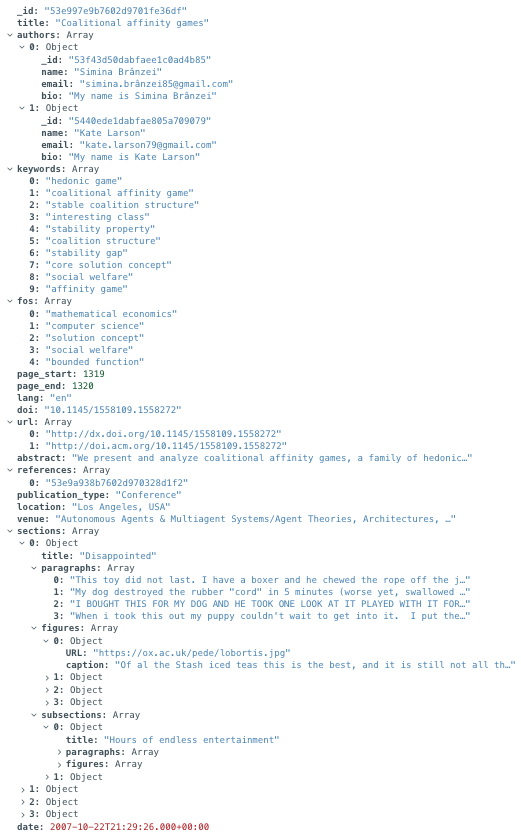
\includegraphics[width=0.9\linewidth]{ImagesMongoDB/conference}
        \label{fig:conference}%
    \end{center}
\end{figure}


\section{Differences concerning the previous models}
\label{sec:differences_concerning_the_previous_models}%
The main advantage of this approach is the fact that it is very easy to get all the relevant data of an article because all the information is stored together and usually allows to avoid performing expensive joins that would be necessary using a relational database.

Furthermore, MongoDB is flexible permitting to have heterogeneous documents, we need to maintain the same skeleton for all documents in the same collection to perform meaningful queries and have a clean database, but also differences between documents are admitted.
As highlighted in the notes above, different types of articles can have different fields and if an article doesn't have certain data is not necessary to store an empty field, simply the attribute is not created.
In addition, this flexibility makes easy the storage of the text structure that could, in principle, have many levels of subsections.

One drawback is the duplication of data, for example, an author may have written more than one paper that is stored in the database, so the author's information is saved multiple times.
This situation could lead to some inconsistency and requires attention when data updates are performed.
But, in the field of bibliography, it is seldom necessary to do updates since all data refer to a specific article and if a paper is modified it is more probable to create a new document with the new version than update the older one.


\chapter{Data upload}
\label{ch:data_upload_mongodb}%


\section{Pre-processing}
\label{sec:pre_processing_mongodb}%
The assignment for this part of the project defined a basic structure of the document with the fields it must have.
Some of the fields defined by this structure were not present in our previous dataset so we had to fix this aspect by doing some pre-processing of the data before working with it.
The starting point has been the dblp dataset, cleaned with python scripts just like in the Neo4j part, but also enriched with new information and new filters on the data.
In particular, the main work revolved around the following fields.

\paragraph{Author email and bio}
Using a Python script, we added the emails of the authors adopting the following format:
\begin{lstlisting}[label={lst:author_email}]
author.name + last-two-digits-of-the-author._id + "@gmail.com"
\end{lstlisting}
Using the same script, we added the bio using the format:
\begin{lstlisting}[label={lst:author_bio}]
"My name is " + author.name + "." + "I'm currently working for " + author.org
\end{lstlisting}
The second sentence, \verb|'"I'm currently working for " + author.org'| is present only if the author has an affiliation.

Then we generated random dates adopting the format \verb|ISODate| of \verb|MongoDB| from \href{https://www.mockaroo.com}{mockaroo.com} and added them to the original dataset with a Python script.

\paragraph{Sections and subsections}
The sections and subsections fields, as mentioned in the assignment instructions were mandatory for the document structure.
However, the documents in our dataset didn't have those fields so we had to manually generate them.
We did so by using a Python script.
More specifically the titles of the sections and subsections and the text for the paragraphs were extracted from the fields \verb|Summary| and \verb|Text| respectively, present in an external dataset named \verb|Reviews.csv|\footnotemark\footnotetext{Amazon Fine Food Reviews, accessed on the 14/11/2022\\
\indent\indent https://www.kaggle.com/datasets/snap/amazon-fine-food-reviews}, which consists of food reviews from Amazon.
The script first generates a set of unique sections with a random number of paragraphs and a random number of subsections, which are themselves sections but without a subsections field (the boundaries of this random number were tuned in the script).
We decided to maintain only a level of subsections to have a more concise document that satisfies the requirements.
Secondly, a (bounded) random number of sections were added to each paper document of the original dataset.

\paragraph{URLs and captions} Images URLs have been generated from \href{https://www.mockaroo.com}{www.mockaroo.com}, while captions are from the \verb|Summary| field of the same dataset \verb|Reviews.csv| used to generate the sections.
We wrote a Python script to add both values to the original dataset.

\paragraph{Venue} The \verb|venue| field was generated from the \verb|venue.raw| given by the initial dataset.
In the version of the \verb|dblp| that we downloaded the venue was a composed field with a lot of information, such as the \verb|raw|, the \verb|name|, the \verb|_id|, and the \verb|type|.
We chose to maintain only the \verb|raw|, which encoded the more interesting data and we assigned it to the field named \verb|venue|.


\section{Upload process}
\label{sec:upload_process_mongodb}%
The upload of the data was quite straightforward since our dataset was already in JSON format.
Since the importing feature of MongoDB was much more efficient than Neo4j we were able to load a much bigger dataset containing 56K documents.

After uploading the data we performed the following filters:
\begin{itemize}
    \item We deleted some fields from all the documents because we were not interested in maintaining all the data, but just the ones that matched more or less the chosen structure for the collection.
    We used the \verb!$unset! command to remove specific fields, such as the \verb|pdf| and the \verb|year|, that was superfluous having the field \verb|date|.
    An example of this procedure is reported in the third command of the following section.
    \item We checked all the fields to remove empty fields, so we cleaned the dataset by removing uninteresting values.
    We executed this cleaning part firstly by checking if the field equals the empty value \verb|""| and then using the \verb|$unset| command on the respective element.
    As before we can see an example of this procedure also in the third command of the following section.
    \item We executed some additional commands to filter the data, from the \verb|FILTERING| option of \verb|MongoDB Compass|, such as the following one:
    \begin{lstlisting}[label={lst:filtering}]
{$and: [
    { title: { $not: { $regex: '^[1-9]' } }},
    { page_start: { $regex: '^[0-9]+$' }},
    { page_end: { $regex: '^[0-9]+$' }},
    { volume : {$not : { $eq : "null"}}},
    { abstract: {$not : {$eq : "null"}}},
]}
    \end{lstlisting}
    Controls similar to the one just reported can be executed at any time, for instance after acquiring some new data from an external source, to have only documents with interesting values.
\end{itemize}


\chapter{Commands and queries}
\label{ch:commands_and_queries_mongodb}%


\section{Commands}
\label{sec:commands_mongodb}%
\begin{enumerate}
    \item \textbf{Inserting a document} \\
    To insert in our database only one document at a time, we use the following function \verb|insertOne()|, which takes in input one document and inserts it in the DB. If the document does not specify an \verb|_id| field, as is our case, then mongod\footnotemark\footnotetext{mongod is the primary daemon process for the MongoDB system} will add the \verb|_id| field and assign a unique \verb|ObjectId()| for the document before inserting it.
    Since when importing this dataset the \verb|_id| were defined as String we decided to explicit the \verb|_id| creation so we can use the \verb|toString()| method to cast it to a String type and be consistent with the data we loaded from the dataset.
    As shown below, for this example we have retrieved a real-world paper and shaped its information to our document structure.
    Firstly, we searched for the author by name and since we didn't find him, we created a new \verb|_id| for him.
    For text formatting reasons in the preview below, we have omitted the values of the \verb|abstract| and \verb|sections| fields.
    The \verb|references| field is an empty array because all the referenced papers by this one are not present in our DB\@.
    \begin{lstlisting}[label={lst:command1mongodb1}]
db.bibliography.insertOne(
{
    _id: ObjectId().toString(),
    title: "Reinforcement Learning for Improving Agent Design",
    authors: [
        {
            _id: ObjectId().toString(),
            name: "David Ha",
            email: "hadavid@google.com",
            bio: "AI resercher at Google Brain, based in Tokyo, Japan",
            org: "Google Brain"
        }
    ],
    abstract: "...",
    keywords: ["computer science", "ai", "reinforcement learning", "cumulative reward", "joint learning"],
    fos: ["computer science", "ai", "reinforcement learning"],
    publication_type: "Journal",
    publisher: "MIT Press Direct",
    venue: "Artificial Life",
    volume: 25,
    issue: 4,
    issn: "352-365",
    date: ISODate('2019-12-02T10:49:36.000'),
    page_start: 23,
    page_end: 46,
    lang: "en",
    doi: "doi.org/10.1162/artl_a_00301",
    url: [
        "https://arxiv.org/abs/1810.03779",
        "https://arxiv.org/abs/1810.03779v3",
        "https://doi.org/10.48550/arXiv.1810.03779"],
    references: [],
    sections: []
})
    \end{lstlisting}
    An easy way to know if the papers referenced by the one we are about to insert are present in the database is to query it using the DOIs of the referenced paper (like is shown in the code snippet below) and then get the \verb|_id| values to be added to the references.
    \begin{lstlisting}[label={lst:command1mongodb2}]
db.bibliography.aggregate([{
    $match: {
        doi: {$in: [
            "10.1109/CMPSAC.2002.1044548",
            "10.1007/s11704-011-0127-6",
            "10.1016/j.datak.2008.09.003"
            ]}}}, {
    $project: {"_id": 1}}
])
    \end{lstlisting}
    Using the database structure presented earlier, we realized that managing the data could not be so straightforward, especially when a new document insertion is required.
    These drawbacks are due to the data sources we had because only a small percentage of the papers had the values for DOI and ORCID but we would have shrunk too much our dataset keeping only those articles.
    In a further improved version, some precautions could be taken to have a more clean and easy-to-use database if the DOI field is known for all documents and the ORCID for all authors.

    With the above assumptions, we could use the DOI for the references because it is a globally unique and independent identifier usable in any database implementation.
    In this way, it would be easier to insert a new document because the new paper could be added to the collection even if the references are not present in the dataset, and the related papers could be inserted afterward.
    Likewise, using the ORCID as the author identifier would also make it easier to add new documents because the ORCID has the same global uniqueness property.
    It would not be necessary to check if the author is already present in the database to set the same id, risking creating inconsistency, but we could insert it just as it is.

    Despite the further checks required in our implementation, when adding the document, we decided to avoid imposing too many limitations on the structure of the data.
    If the papers have the DOI and the authors have the ORCID is easier to search the collection, but we cannot guarantee the presence of these fields, so to have a more flexible database, we accept papers without DOI and ORCID. A less bounded dataset leads to the necessity of adding some checks to maintain data consistency and requires being more careful when inserting data to avoid duplication.
    \item \textbf{Update a single document} \\
    The command \verb|updateOne| allows one to search for a document that matches a specific filter and modifies it accordingly to the update rules expressed inside the query.
    In general, the command modifies only the first found document, but if no document matches the search, then no changes are applied to the database.

    The \verb|$set| operator sets a new value for the specified attribute or creates it if it does not exist.
    The \verb|$unset| operator deletes a specified document attribute if the document has the field otherwise, nothing changes.
    The following command might be useful when new data regarding papers become available or when some information needs to be updated due to mistakes.
    The command allows to find a document with the field \verb|_id| equal to \verb|"53e997bab7602d9701fa09cb"| and changes its field \verb|publication_type| to \verb|"Conference"| because this is its actual type and also changes its field \verb|publisher| to \verb|"Association of Forensic Document Examiners"| with the command \verb|$set|.
    This operator is also used to create the field \verb|location| to which is assigned the value \verb|"Grenoble, France"|.
    The update part of the query also allows the removal of the fields \verb|page_start| and \verb|page_end| by using the command \verb|$unset|.
    \begin{lstlisting}[label={lst:command2mongodb}]
db.bibliography.updateOne( {
    _id: "53e997bab7602d9701fa09cb" }, [ {
        $set: { publication_type: "Conference" } }, {
        $set: { publisher: "Association of Forensic Document Examiners" } }, {
        $set: { location: "Grenoble, France" } }, {
        $unset: [
            "page_start",
            "page_end" ] } ] )
    \end{lstlisting}
    \begin{figure}[H]
        \begin{center}
            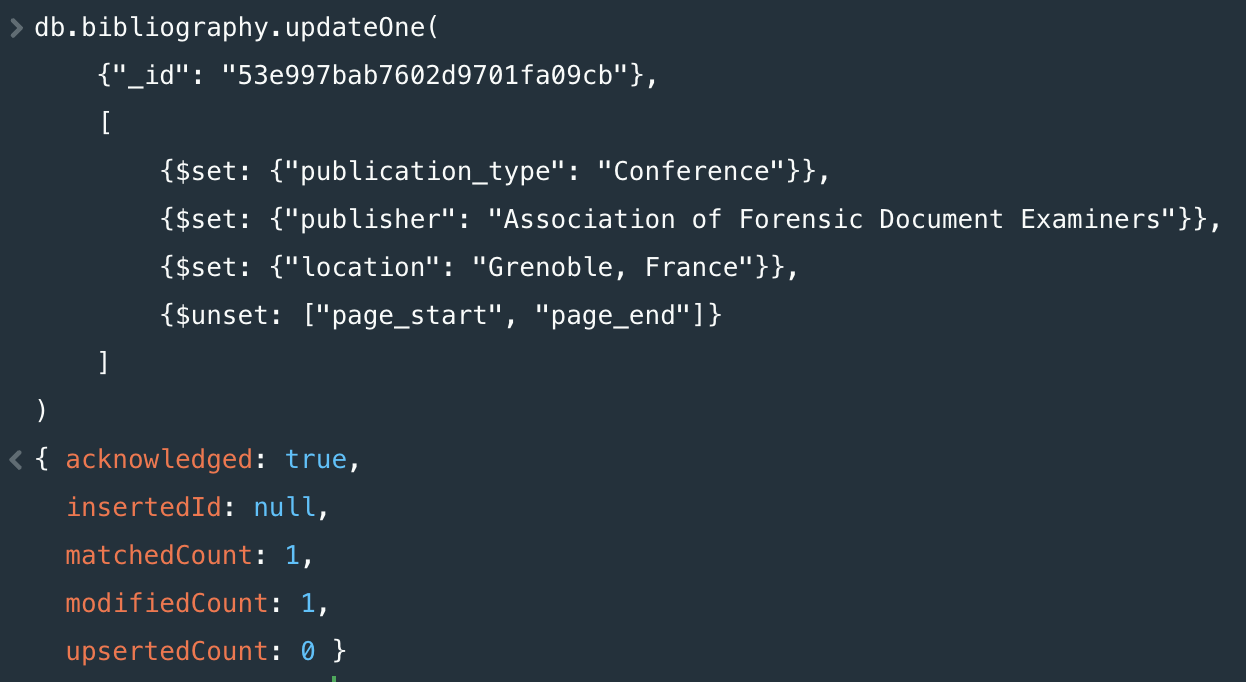
\includegraphics[width=0.9\linewidth]{ImagesMongoDB/command2mongo}
            \label{fig:command2mongodb}%
        \end{center}
    \end{figure}
    In this case, only one document could have been found because the field \verb|_id| is the unique identifier.
    It is necessary to be careful in updating the database in order to avoid updating the wrong documents, deleting fields, and changing important values.

    Another important use case of \verb|updateOne| is associated with the need to replace a document with a different one.
    This exchange can be done using the operator \verb|$replaceWith| and specifying the document to remove and the one that has to be put inside the database instead of it.
    \item \textbf{Remove fields} \\
    Uploading the dataset, as we previously explained in the chapter about the upload process, we ended up with a lot of data, some of which were not of our interest.
    Using the following command we consider all the data entries of the collection \verb|bibliography| and without any filtering, we just remove the \verb|year| field from all the documents.
    We decided to remove this field because we already have the \verb|date| so this is unnecessary.
    \begin{lstlisting}[label={lst:command3mongodb1}]
db.bibliography.updateMany( {
    }, {
    $unset: { year: "" } } )
    \end{lstlisting}
    In order to maintain only interesting values about the papers, we also remove the empty fields.
    It doesn't make sense to keep fields that are equal to an empty value, so, for instance, if \verb|doi| is just an empty string, we delete it from the respective document.
    We keep only useful data that respect the structure of the dataset we want to work with to extract knowledge.
    We executed the following command for all the fields for the sake of having a clear collection.
    \begin{lstlisting}[label={lst:command3mongodb2}]
db.bibliography.updateMany( {
    doi: { $eq: "" } }, {
    $unset: { doi: "" } } )
    \end{lstlisting}
    \item \textbf{Delete a group of documents} \\
    The command \verb|deleteMany()| deletes a group of documents that match the condition given inside the specified filter.
    In this case, the documents that have as date one that occurs before the \verb|1950| are considered obsolete, so we want to delete them.
    For this reason, it's enough to execute a check on the field \verb|date|, that is of date type, so we have to specify the \verb|ISODate| format and delete all the documents previous to \verb|'1950-01-01T00:00:00.000Z'|.
    \begin{lstlisting}[label={lst:command4mongodb}]
db.bibliography.deleteMany( { date: { $lt: ISODate("1950-01-01T00:00:00.000Z") } } )
    \end{lstlisting}
    After executing the command successfully, \verb|MongoDB| acknowledges the write operation and returns the number of documents that were eliminated from the collection.
    \begin{figure}[H]
        \begin{center}
            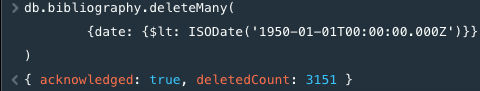
\includegraphics[width=0.6\linewidth]{ImagesMongoDB/delete}
            \label{fig:delete}%
        \end{center}
    \end{figure}
    \item \textbf{Update a group of documents} \\
    The command \verb|updateMany| allows the modification of multiple documents at the same time.
    Since in the database some articles have \verb|"Elsevier"| as \verb|publisher|, and some others have \verb|"Elsevier Ltd."|, and since both values represent the same publisher, we want to merge them.
    With the following command, all documents that have value \verb|"Elsevier Ltd."| in the field \verb|publisher| are retrieved, then the value is changed in \verb|"Elsevier"|.
    \begin{lstlisting}[label={lst:command5mongodb}]
db.bibliography.updateMany( {
    publisher: "Elsevier Ltd." }, {
    $set: { publisher: "Elsevier" } } )
    \end{lstlisting}
    \begin{figure}[H]
        \begin{center}
            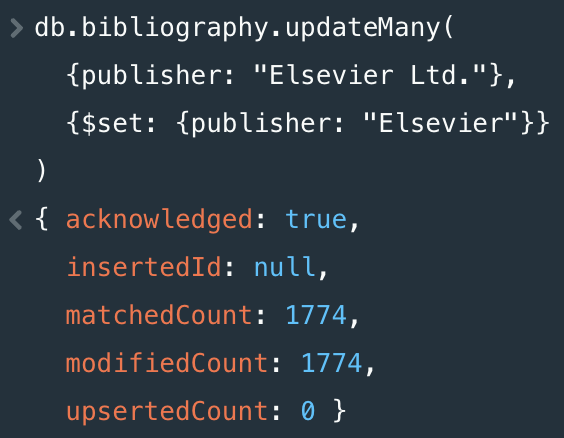
\includegraphics[width=0.45\textwidth]{ImagesMongoDB/command5mongodb}
            \label{fig:command5mongodb}%
        \end{center}
    \end{figure}
\end{enumerate}


\section{Queries}
\label{sec:queries_mongodb}%
\begin{enumerate}
    \item \textbf{Papers published in a certain period on a specific type of publication} \\
    The query's goal is to find all the papers published in a particular time frame delimited by two dates (included) of a type of publication, such as a journal.
    More specifically, the search is conducted on papers published between January 2005 and December 2010 in journals.
    To be compliant with the data type of the \verb|date| field, the date must be specified in a \verb|ISODate| format.
    In the projection, we only show \verb|title| and \verb|venue| of a paper, that is the name of the Journal, and we suppress the field \verb|_id| because not informative.
    \begin{lstlisting}[label={lst:query1mongodb}]
db.bibliography.find( {
    $and: [ {
        date: { $gte: ISODate('2005-01-01T00:00:00.000Z') } }, {
        date: { $lte: ISODate('2010-12-31T00:00:00.000Z') } }, {
        publication_type: "Journal" } ] }, {
    _id: 0,
    title: 1,
    venue: 1 } ).limit(5)
    \end{lstlisting}
    \begin{figure}[H]
        \begin{center}
            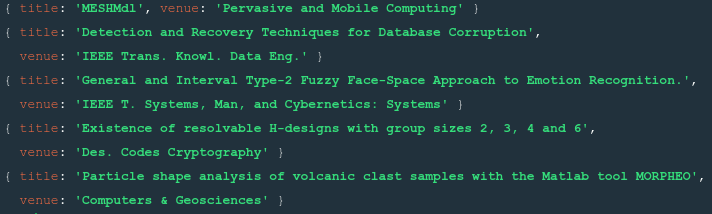
\includegraphics[width=0.9\linewidth]{ImagesMongoDB/query1mongodb}
            \label{fig:query1mongodb}%
        \end{center}
    \end{figure}

    \paragraph{Performance:}
    It's obvious to see that this query iterates through the values of a field to filter some documents.
    If the time range inserted to do the query is small, we can say that the query is highly selective, that is, a query that returns only a few documents from the whole set of scanned documents.
    Selective queries are the ones that make the best usage of indexes, so we thought to do a comparison test of the performance of the query with and without an index on the date.\\
    To have a more meaningful result for the test we removed the \verb|db.collection.limit()| function, otherwise, the automatic rearrangement of the queries would limit the query to stop as soon as it matches 5 correct instances.
    With this limit on the query, the load on the system would be so light that we would see a negligible difference between the query run with and without the indexes.\\
    To get information about the query performance we use \verb|db.collection.explain()|, which returns information about the query plan.
    Passing the \verb|executionStats| argument to this method makes it return an additional section where a set of useful performance markers are shown.

    \paragraph{Results}
    We first try running the query without an index on the field \verb|date|.
    Using the method \verb|explain| with the argument \verb|executionStats| we get the following result (we show only a selection of the markers present in the \verb|executionStats| section, the ones meant for this discussion):
    \begin{figure}[H]
        \begin{center}
            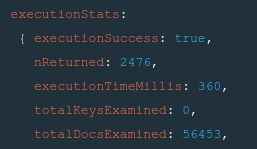
\includegraphics[width=0.45\linewidth]{ImagesMongoDB/result_query1mongodb1}
            \label{fig:result_query1mongodb1}%
        \end{center}
    \end{figure}
    MongoDB runs the query optimizer to choose the winning plan, executes the winning plan to completion, and returns statistics describing the execution of the winning plan.
    In the reported results we can see different parameters that explain the query, and among these, we focus our comparison, especially on the following:
    \begin{itemize}
        \item \verb|nReturned|: number of documents that match the query condition
        \item \verb|executionTimeMillis|: total time in milliseconds required for query plan selection and query execution
        \item \verb|totalKeysExamined|: number of index entries scanned
        \item \verb|totalDocsExamined|: number of documents examined during query execution
    \end{itemize}
    We can clearly see that the documents passing the filter are about 4\% of the total, so we can say that this query is selective enough and can proceed to test it with the addition of an index.
    We'd like also to point out that the \verb|totalKeysExamined| parameter has a value of 0, meaning that this query has not performed a search on indexes.
    Meanwhile, the \verb|totalDocsExamined| shows that all the documents in the DB were examined.
    We proceed to create an index on the field \verb|date| and we run the query again.
    This time the execution plan and stats return different values:
    \begin{figure}[H]
        \begin{center}
            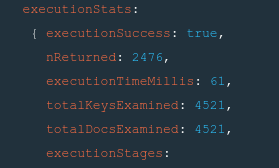
\includegraphics[width=0.45\linewidth]{ImagesMongoDB/result_query1mongodb2}
            \label{fig:result_query1mongodb2}%
        \end{center}
    \end{figure}
    We can immediately notice that the execution time has gone down to 61ms from the 360ms of before, a performance gain of more than 5x.
    Since the indexes are stored in an ordered way the query executioner can iterate through the dates with a much faster binary search algorithm.
    This means we have to do a much smaller number of accesses to the keys of the database, as shown by the value of \verb|totalKeysExamined| parameter in the figure.
    In this particular case, we also have to access the DB (as shown by the \verb|totalDcosExamined| parameter) because the \verb|publication_type| field is not stored in an index, so we have to retrieve the value of this field from the document itself to complete the filtering condition\footnotemark\footnotetext{This type of query, where not all the field needed to compute the query are stored as indexes are called "not covered queries"}.
    Nonetheless, the much lower number of accesses to DB provided by the index on \verb|date| is sufficient to experience a significant gain in performance.
    \item \textbf{Search a given word inside the title of papers written on books and published by a specific publisher} \\
    MongoDB supports query operations that perform a text search, but to enable this functionality is necessary to define a textual index that makes the search possible.

    To achieve more efficient execution of queries, we can define indexes, which are data structures that store useful information to speed up the search.
    When MongoDB executes a query without indexes, it has to evaluate the conditions on all the documents of the considered collection.
    If an index is defined and used, MongoDB can limit the number of analyzed documents and requires less time to compute the results.
    The following command is necessary for creating indexes, and it is essential before executing the following query.
    \begin{lstlisting}[label={lst:query2mongodb1}]
db.bibliography.createIndex( { title: "text" } )
    \end{lstlisting}
    \begin{figure}[H]
        \begin{center}
            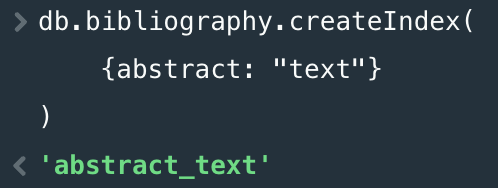
\includegraphics[width=0.45\linewidth]{ImagesMongoDB/query2mongodb1}
            \label{fig:query2mongodb1}%
        \end{center}
    \end{figure}
    Once the index is created, the query can be run.
    It returns the titles of the documents whose title presents the word \verb|"software"| and that were published in a book by the publisher \verb|"Elsevier"|.
    \begin{lstlisting}[label={lst:query2mongodb2}]
db.bibliography.find( {
    $text: { $search: "software" },
    publication_type: "Book",
    publisher: "Elsevier" }, {
    title: 1 } ).limit(5)
    \end{lstlisting}
    \begin{figure}[H]
        \begin{center}
            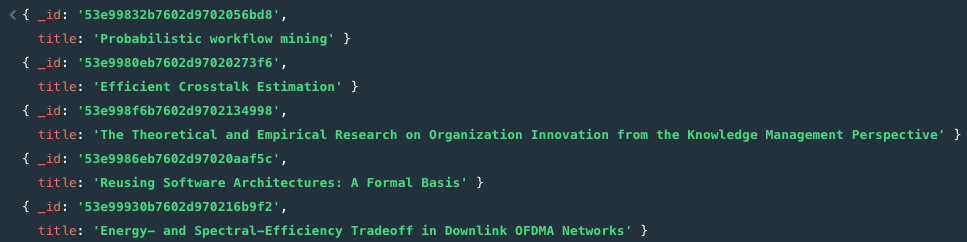
\includegraphics[width=0.9\linewidth]{ImagesMongoDB/query2mongodb2}
            \label{fig:query2mongodb2}%
        \end{center}
    \end{figure}
    \item \textbf{Visualize the common values between the field of study and keywords in each document} \\
    The following query extracts all those documents with at least one keyword as their field of study.

    In particular, we project \verb|title|, \verb|fos|, \verb|keywords|, and their sizes, and then we find all those documents that contain more than thirty keywords, and more than fifteen fields of study.
    We select such a huge number of fields of study and keywords because we are interested in papers that are involved in research that can be important in many areas.

    Finally, we project again \verb|title| and the intersection set between keywords and fields of study to extract and show the ones that match.
    \begin{lstlisting}[label={lst:query3mongodb}]
db.bibliography.aggregate( [ {
    $project: {
        title: "$title",
        fos: "$fos",
        keywords:"$keywords",
        fosSize: { $size: "$fos" },
        keywordsSize: { $size: "$keywords" } } }, {
    $match: { $and: [ {
        keywordsSize: { $gt: 30 },
        fosSize: { $gt: 15 } } ] } }, {
    $project: {
        title: "$title",
        intersection: { $setIntersection: [
            "$fos",
            "$keywords" ] } } } ] )
    \end{lstlisting}
    \begin{figure}[H]
        \begin{center}
            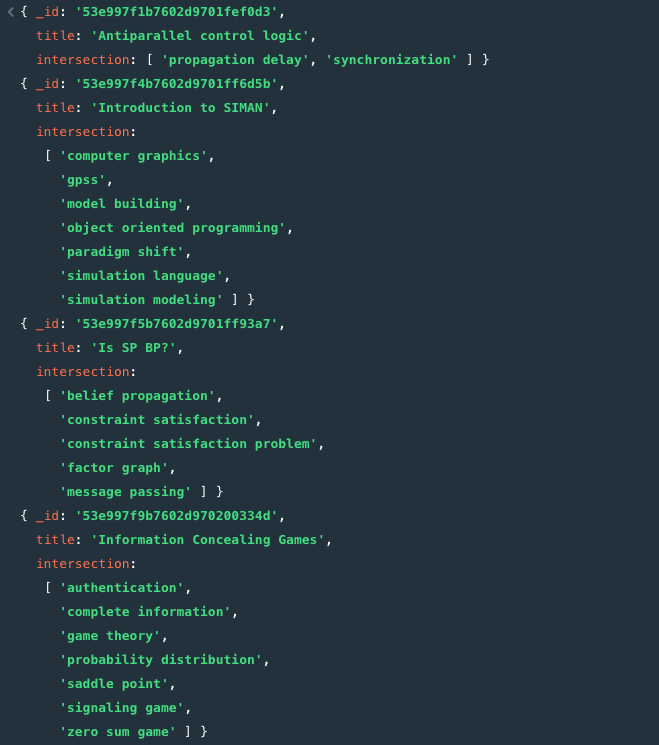
\includegraphics[width=0.9\linewidth]{ImagesMongoDB/query3mongodb}
            \label{fig:query3mongodb}%
        \end{center}
    \end{figure}

    \paragraph{Performance:}
    Let's first consider the query just explained with the relative outcome of the execution, using \verb|explain("executionStats")| in order to analyze its performance:
    \begin{lstlisting}[label={lst:performance_query3mongodb}]
db.bibliography.aggregate( [ {
    $project: {
        title: "$title",
        fos: "$fos",
        keywords:"$keywords",
        fosSize: { $size: "$fos" },
        keywordsSize: { $size: "$keywords" } } }, {
    $match: { $and: [ {
        keywordsSize: { $gt: 30 },
        fosSize: { $gt: 15 } } ] } }, {
    $project: {
        title: "$title",
        intersection: { $setIntersection: [
            "$fos",
            "$keywords" ] } } } ] ).explain("executionStats")
    \end{lstlisting}
    The query firstly scrolls through all the documents, just selecting some fields that we want to project and calculating the size of the \verb|fos| and of the \verb|keywords|.
    In the execution, this is shown by the fact that all the documents that are examined at this first step are also returned.
    This procedure has as \verb|explain.executionStats.| \verb|executionTimeMillis| a value of \verb|633 ms| and doesn't reduce the papers to work on.
    We can also see from the \verb|explain.executionStats.| \verb|totalKeysExamined| that the number of index entries is zero because we don't use any indexing on the fields involved.
    \begin{figure}[H]
        \begin{center}
            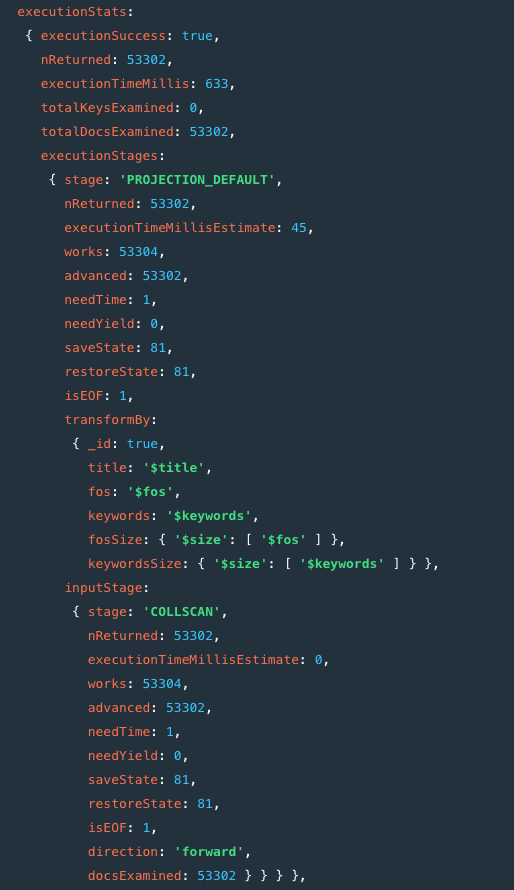
\includegraphics[width=0.6\linewidth]{ImagesMongoDB/performance_query3mongodb1}
            \label{fig:performance_query3mongodb1}%
        \end{center}
    \end{figure}
    After the scrolling, we execute a \verb|match| that narrows down the papers and reduces the computation.
    As follows, we can see that this part of the query requires also \verb|610 ms|, given the fact that has to analyze again all the documents, but after the execution, only \verb|9| matching papers are returned, and shown with the projection.
    \begin{figure}[H]
        \begin{center}
            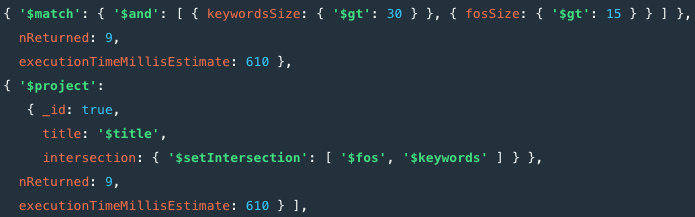
\includegraphics[width=0.9\linewidth]{ImagesMongoDB/performance_query3mongodb2}
            \label{fig:performance_query3mongodb2}%
        \end{center}
    \end{figure}
    Given the fact that the query examined so far has to scroll over all the documents twice, we thought of the following alternative, that first executes the \verb|match| part and then shows the intersection between the \verb|fos| and the \verb|keywords|, without using two projections.
    \begin{lstlisting}[label={lst:performance_query3mongodb3}]
db.bibliography.aggregate( [
    {$match: {
        $expr: {
            $and: [ {
                $gt: [{$size: "$keywords"}, 30 ] }, {
                $gt: [{$size: "$fos"}, 15]
                } ] } } } , {
    $project: {
        title: "$title",
        intersection: { $setIntersection: [
            "$fos",
            "$keywords" ] } } } ] ).explain("executionStats")
    \end{lstlisting}
    As before the query starts examining all the documents of the collection and we have no index entries, not having any index on the involved fields.
    We can see some important differences from the previous procedure looking at mainly two fields of the \verb|explain.executionStats| reported below.
    We can understand from the \verb|explain.executionStats.executionTimeMillis| that the execution time is lower, requiring only \verb|246 ms|, doing the filtering of the papers as the first action of the query.
    Afterward, the projection of the result required only \verb|24 ms|, because the documents were already narrowed down.
    In fact, we can notice that the \verb|match| examined all the collections, but returned only \verb|9| matches, exactly like before, only now this operation was done before any other, so it improved the overall execution.
    \begin{figure}[H]
        \begin{center}
            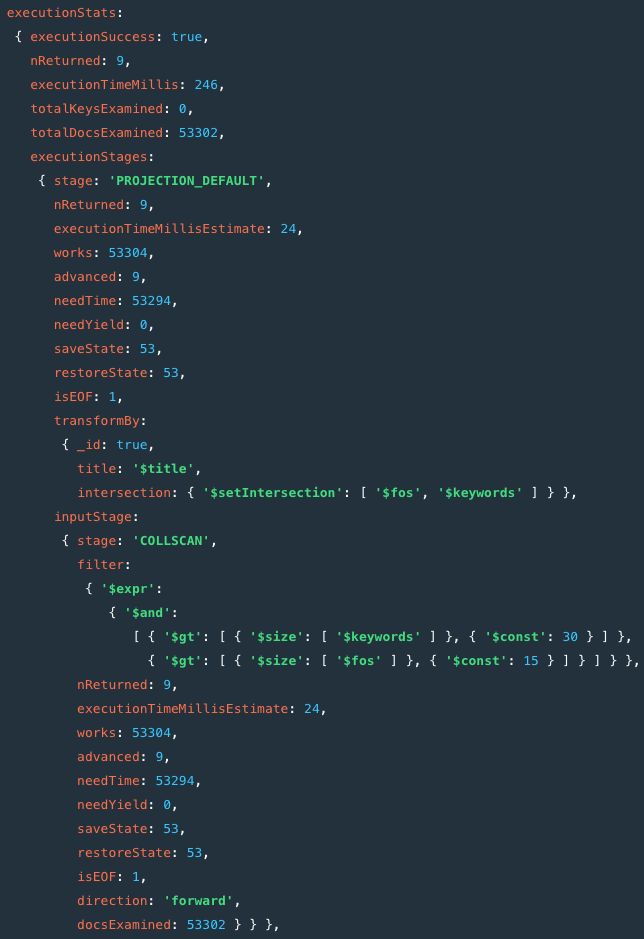
\includegraphics[width=0.6\linewidth]{ImagesMongoDB/performance_query3mongodb3}
            \label{fig:performance_query3mongodb3}%
        \end{center}
    \end{figure}
    In conclusion, this alternative query is more efficient than the previous one, requiring less time to compute.
    From this analysis we noticed that is better to execute the filtering part, the \verb|match|, as soon as possible in the query, in order to reduce the number of documents we have to work on, speeding up the process since the operations are executed like a pipeline.
    \item \textbf{Organizations that held more conferences in the same location} \\
    The following query matches all the papers that are of type \verb|Conference|.
    We select only the events held by the \verb|"IEEE Global Telecommunications Conference| \verb|(Globecom)"| then for each author involved in the conference, we check the affiliation.
    After every step of the query, we obtain a new temporary collection of documents.
    For instance, with the \verb|unwind| command, we deconstruct the array of \verb|authors| from the input papers to output a new document for each element and, in this way, we create a much bigger dataset.

    With this query, we are interested in knowing how many times an organization held a conference in a specific location through one of its members.
    Regrouping the data by conference location and affiliation of the author involved, we can count the number of times the organization took part in an event held there.
    Finally, the result is sorted by the number of engagements and limited only to the first more active organizations.
    \begin{lstlisting}[label={lst:query4mongodb}]
db.bibliography.aggregate( [ {
    $match: { $and: [ {
        publication_type: { $eq: "Conference" } }, {
        venue: { $eq: "IEEE Global Telecommunications Conference (Globecom)" } } ] } }, {
    $unwind: "$authors" }, {
    $group: {
        _id : {
            location: "$location",
            organization: "$authors.org" },
        locationPerOrganization: { $sum: 1 } } }, {
    $project: {
        location: "$location",
        author: "$organization",
        locPerOrgConference: "$locationPerOrganization" } }, {
    $sort: { locPerOrgConference : -1 } }, {
    $limit: 5 } ] )
    \end{lstlisting}
    \begin{figure}[H]
        \begin{center}
            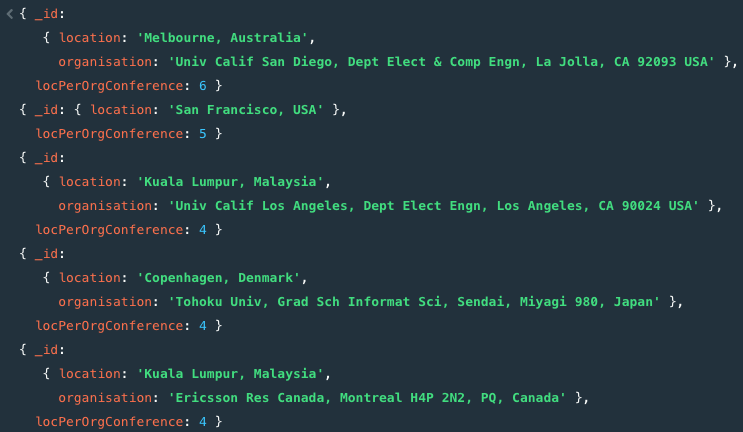
\includegraphics[width=0.9\linewidth]{ImagesMongoDB/query4mongodb}
            \label{fig:query4mongodb}%
        \end{center}
    \end{figure}
    \item \textbf{Papers with a pattern structure} \\
    With this query, we count the number of documents that satisfy a given pattern specified in the \verb|$match| part of the query.
    In this example, we are searching for papers with four sections, and at least one must have four paragraphs, four figures, and one subsection with just one paragraph.
    Using \verb|$size|, it's possible to check the dimension of an array, while using \verb|$elemMatch| is possible to define the criteria that at least one document in an array must satisfy.
    Finally, through the dot notation, we can access a field of an embedded document.
    \begin{lstlisting}[label={lst:query5mongodb}]
db.bibliography.aggregate( [ {
    $match: { $and: [ {
        sections: { $size: 4 } }, {
        sections: { $elemMatch: {
            paragraphs: { $size: 4 },
            figures: { $size:4 },
            subsections: { $size: 1 },
            "subsections.paragraphs": { $size: 1 } } } } ] } }, {
    $group: {
        _id: true,
        count: { $sum: 1 } } } ] )
    \end{lstlisting}
    \begin{figure}[H]
        \begin{center}
            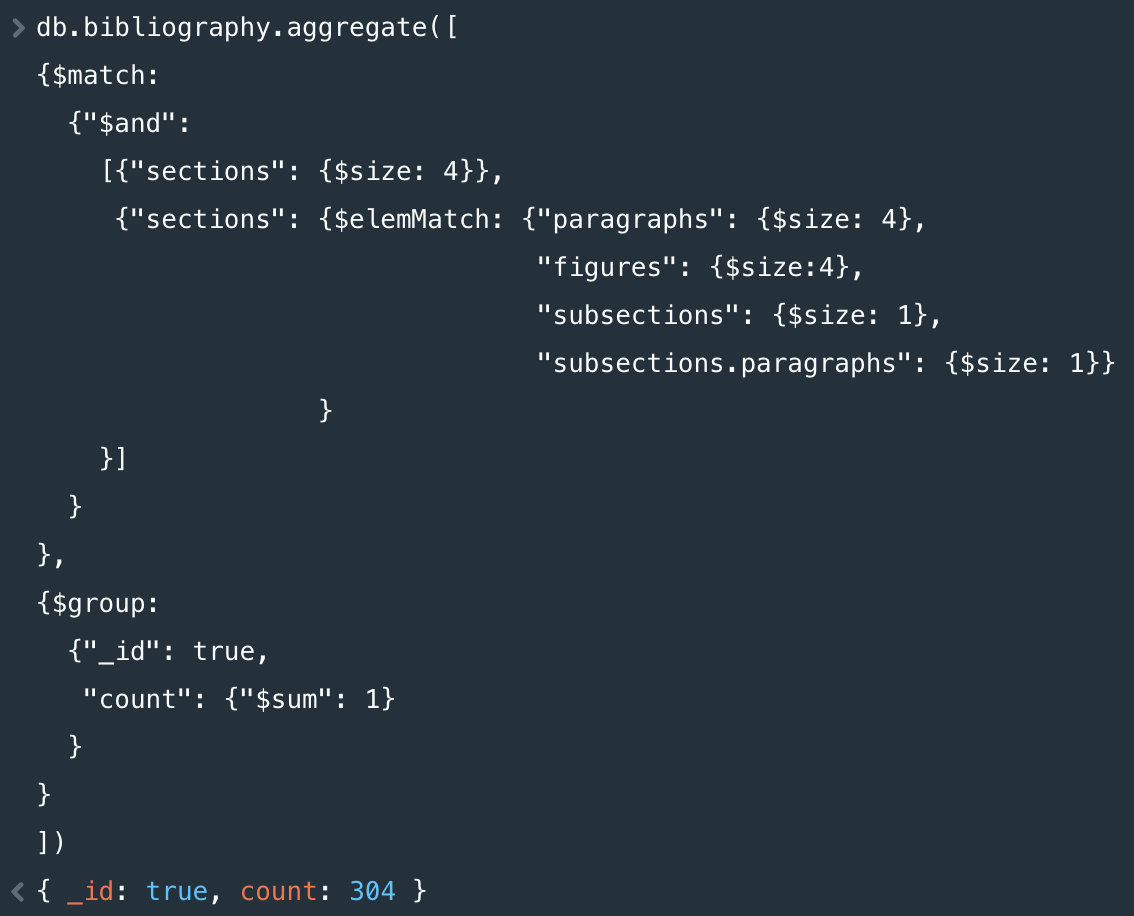
\includegraphics[width=0.6\linewidth]{ImagesMongoDB/query5mongodb1}
            \label{fig:query5mongodb1}%
        \end{center}
    \end{figure}
    \textcolor{red}{The following query is a slight change of the previous one just to retrieve a paper with the wanted structure to show that indeed the query works.}
    \begin{figure}[H]
        \begin{center}
            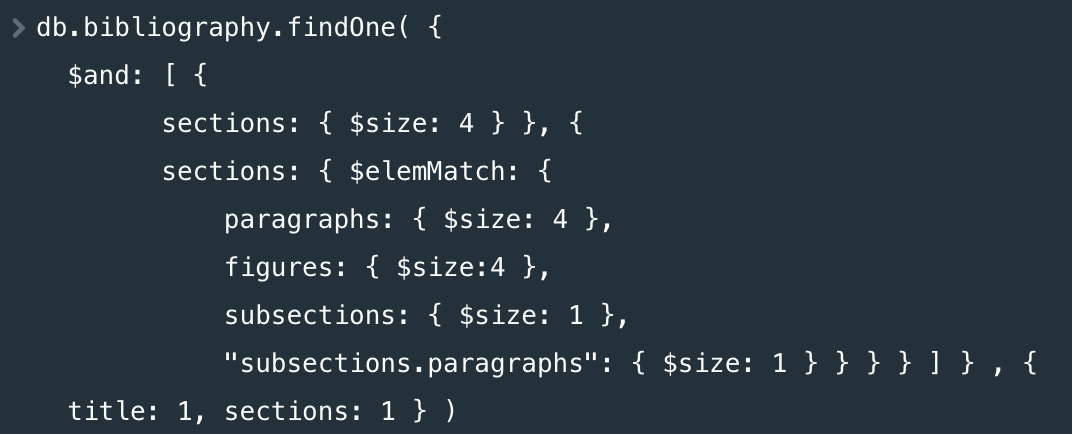
\includegraphics[width=0.6\linewidth]{ImagesMongoDB/query5mongodb2}
            \label{fig:query5mongodb2}%
        \end{center}
    \end{figure}
    \begin{figure}[H]
        \begin{center}
            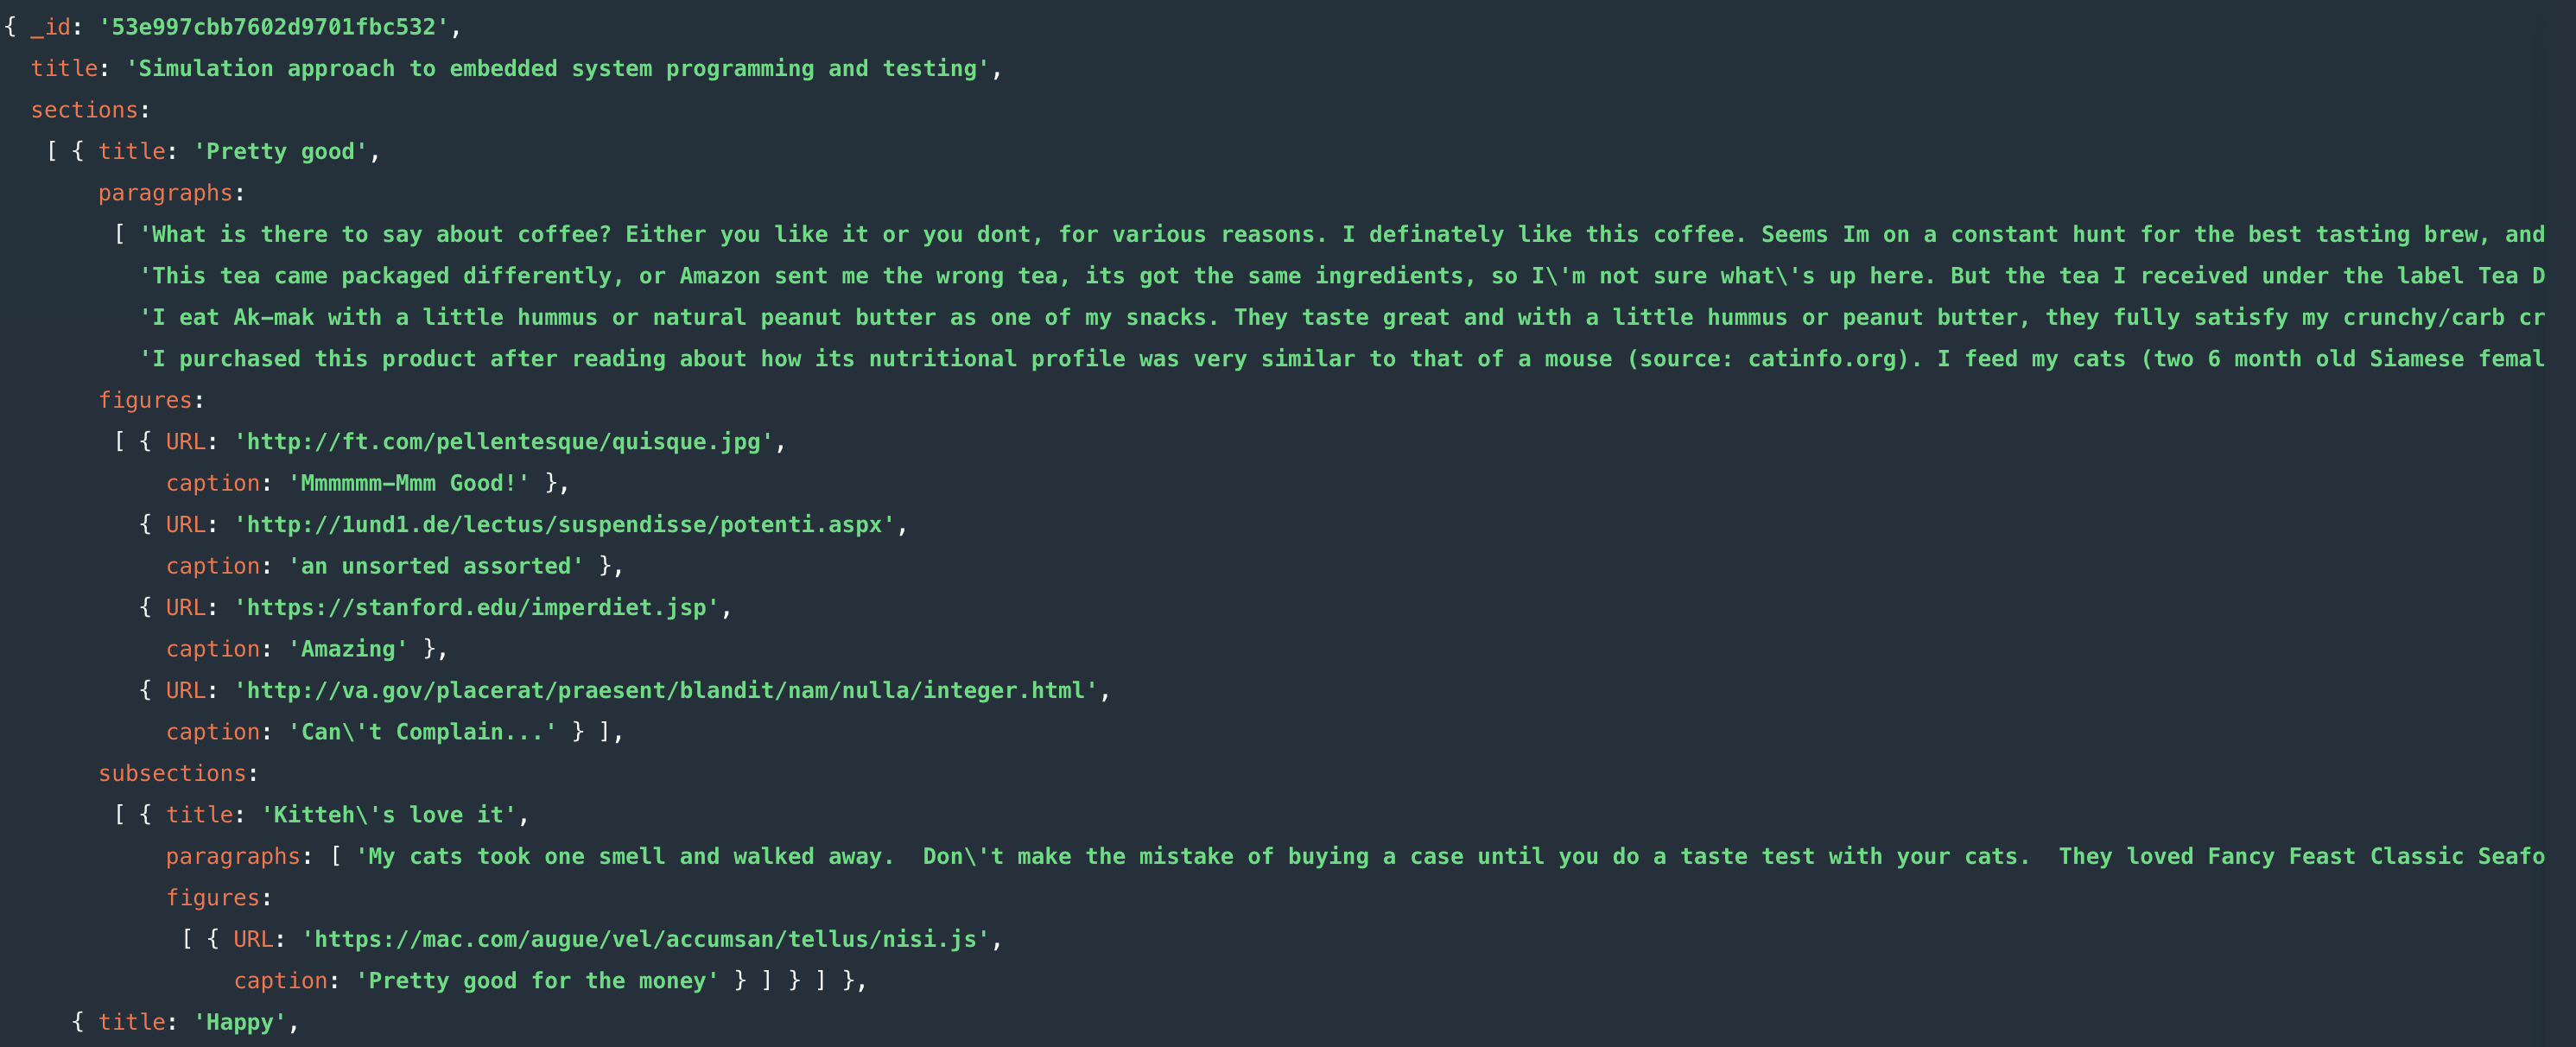
\includegraphics[width=0.9\textwidth]{ImagesMongoDB/result_query5mongodb}
            \label{fig:result_query5mongodb}%
        \end{center}
    \end{figure}
    \item \textbf{Number of papers published by the current staff of an organization} \\
    What we want to achieve with this query is to know how many papers have been published by the researchers working at a certain organization.
    The output list is ordered in descending order, showing the organizations whose researchers have published the most.
    Notice that a paper published by authors from different organizations is counted for all the organizations involved.
    In the first part of the query, we unwind the documents by \verb|authors| and do a filtering of inconsistent data, since the focus of this query is to know which organizations have published the most.
    Secondly, we proceed by grouping documents by the author affiliation (\verb|authors.org|) and the paper itself.
    This operation is needed to filter out the documents referring to the same paper and written by authors that are affiliated with the same organization.
    If we hadn't done this, the same paper would have been counted multiple times, for all the authors who participated in writing it and that are part of the same organization, inflating that organization's contribution.
    Notice that in the result an organization with name \verb|"Corresponding author."| appears, probably this value has been used by the maintainer of the DB to denote independent authors or authors for whom the affiliated organization was not known.
    \begin{lstlisting}[label={lst:query6mongodb}]
db.bibliography.aggregate( [ {
    $unwind: "$authors" }, {
    $match: { $and: [ {
        "authors.org": { $ne: null } }, {
        "authors.org": { $ne: '' } } ] } }, {
    $group: {
        _id: {
            org: "$authors.org",
            p_id: "$_id"} } }, {
    $group: {
        _id: "$_id.org",
        papers: {$sum: 1} } }, {
    $sort: { papers: -1 } }, {
    $limit: 5 } ] )
    \end{lstlisting}
    \begin{figure}[H]
        \begin{center}
            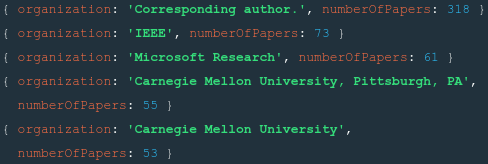
\includegraphics[width=0.9\linewidth]{ImagesMongoDB/query6mongodb}
            \label{fig:query6mongodb}%
        \end{center}
    \end{figure}
    \item \textbf{Number of pages published in Journals by authors affiliated with a certain organization } \\
    This query is similar to the one above, but here we want to retrieve which organizations have contributed the most in writing papers published in journals.
    More specifically, we sum the number of pages written in a specific journal by authors who are currently affiliated with that specific organization.
    This objective is obtained by first unwinding the authors and filtering them to remove some inconsistent data.
    Secondly, we proceed by grouping documents by the author affiliation (\verb|authors.org|) and the paper itself (the other fields of \verb|venue| and \verb|pages| do not contribute to the grouping because they are a single field of the paper document).
    This operation achieves the same goal as the one described in the query before.
    In the second \verb|$group| stage, we group the documents by organization and journal, and we have an accumulator to sum all the pages written by the staff of that organization in that particular journal.
    Finally, the last stages are only for the projection and pretty printing of the output.
    \begin{lstlisting}[label={lst:query7mongodb}]
db.bibliography.aggregate( [ {
    $unwind: "$authors" }, {
    $match: { $and: [ {
        "authors.org": { $ne: null } }, {
        "authors.org": { $ne: '' } }, {
        publication_type: { $eq: "Journal" } }, {
        $expr: { $lte: [
            "$page_start",
            "$page_end" ] } } ] } }, {
        $addFields: { pages: { $subtract: [
            "$page_end",
            "$page_start" ] } } }, {
        $group: { _id: {
            org: "$authors.org",
            paperId: "$_id",
            journal: "$venue",
            pages: "$pages" }, } }, {
        $group: {
        _id: {
            org: "$_id.org",
            journal: "$_id.journal" },
        pages: { $sum: "$_id.pages" } } }, {
    $sort: { pages: -1 } }, {
    $project: {
        organization: "$_id.org",
        journal: "$_id.journal",
        numberOfPages: "$pages" } }, {
    $project: { _id: 0 } }, {
    $limit: 5 } ] )
    \end{lstlisting}
    \begin{figure}[H]
        \begin{center}
            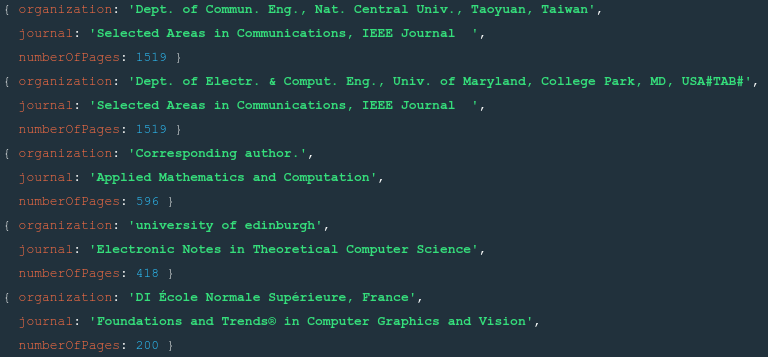
\includegraphics[width=0.9\linewidth]{ImagesMongoDB/query7mongodb}
            \label{fig:query7mongodb}%
        \end{center}
    \end{figure}
    \item \textbf{Couples of the field of study and keyword which appear more frequently within the papers} \\
    The query returns the association between fields of study and keywords which are more present within the database and how many times they appear together.
    Initial filtering is done in order to eliminate the papers which don't contain any keywords or any field of study.
    The two clauses for doing the filtering can be modified by increasing the required number of keywords or the required number of fields of study.
    This kind of change can be interesting in order to understand which fields of study and keywords become more relevant when the subset of the considered paper is different.
    The results are ordered by the number of occurrences of the couples \verb|field of study| - \verb|keyword| by decreasing order.
    This can be done by the operator \verb|"$sort"|.
    We filter out the couples of fields of study and keywords with less than 100 in order to get rid of some misleading information due to not coupled elements.
    The threshold can be adjusted.
    \begin{lstlisting}[label={lst:query8mongodb}]
db.bibliography.aggregate( [ {
    $match: {
        $expr: { $gte: [ { $size: "$fos" }, 0 ] } } }, {
    $match: {
        $expr: { $gte: [ { $size: "$keywords" }, 0 ] } } }, {
    $unwind: { path: "$fos" } }, {
    $unwind: { path: "$keywords" } }, {
    $group: {
        _id: {
            fieldOfStudy: "$fos",
            keyword: "$keywords" },
        keywordsCount: { "$sum": 1 } } }, {
    $match: { "keywordsCount": { $gte: 100 } } }, {
    $sort: { keywordsCount: -1 } }, {
    $limit: 5 }, {
    $project: {
        fieldOfStudy: "$fos",
        keyword: "$keywords",
        score: "$keywordsCount" } } ] )
    \end{lstlisting}
    \begin{figure}[H]
        \begin{center}
            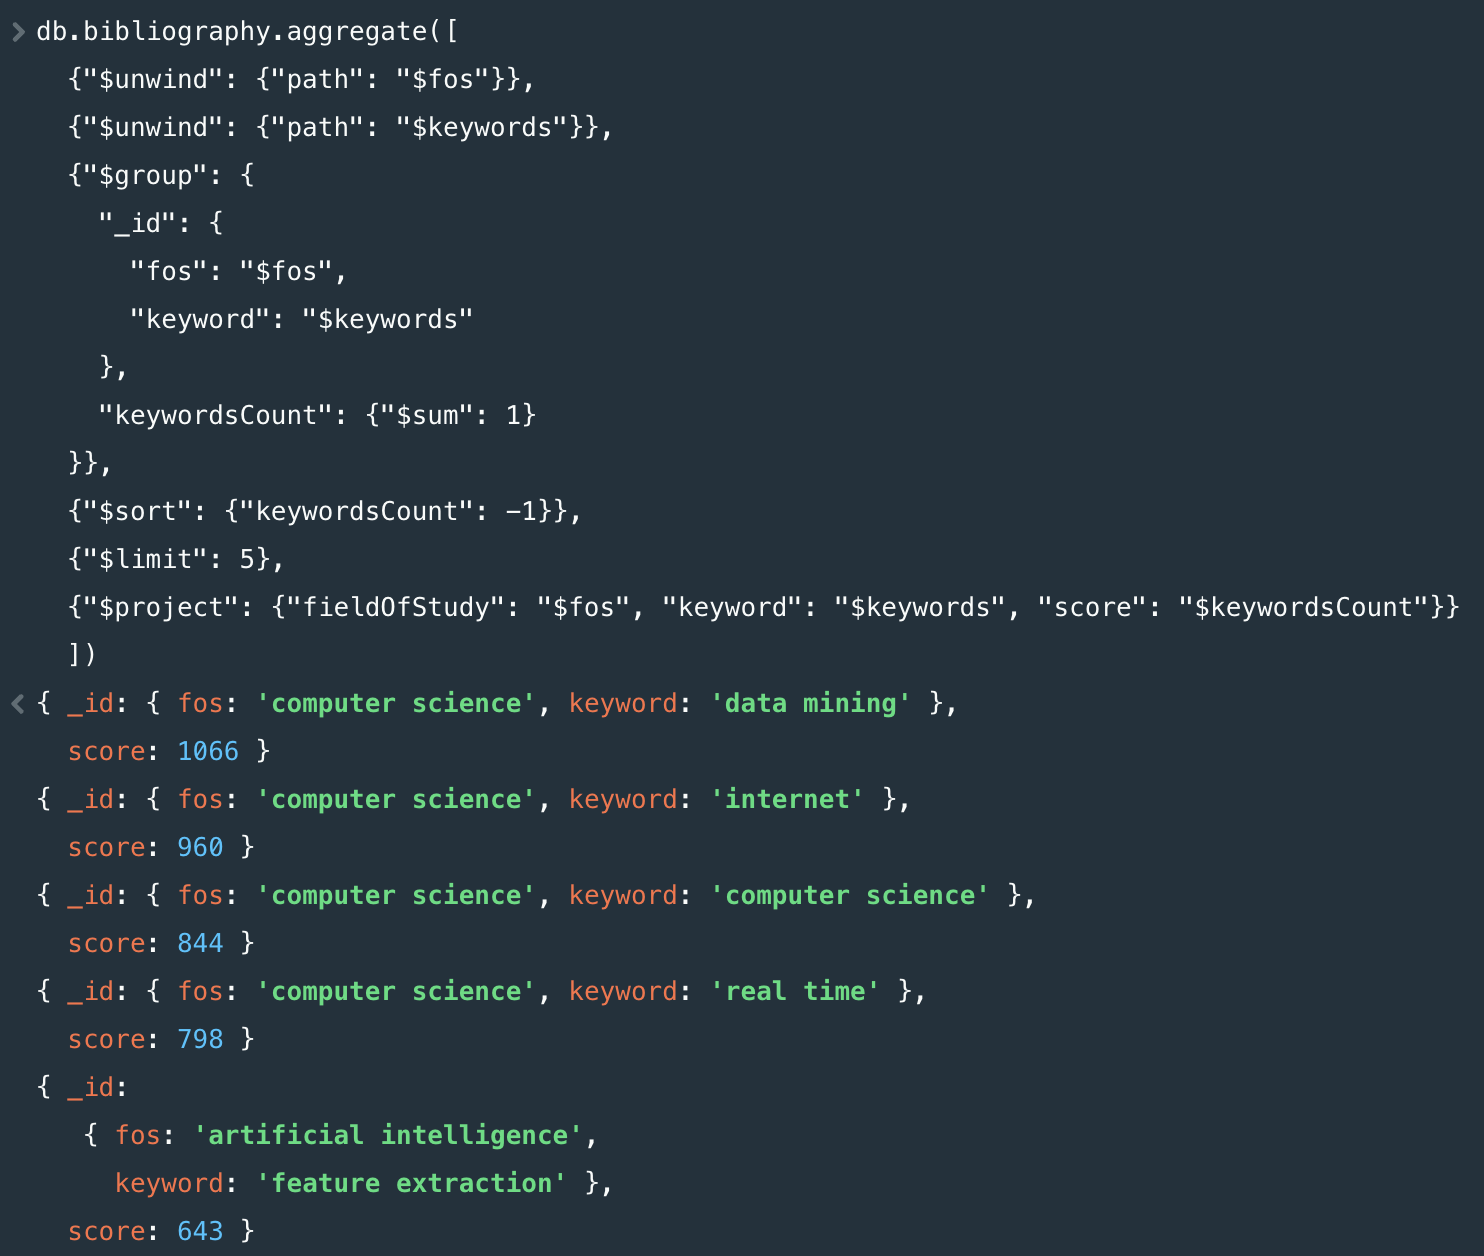
\includegraphics[width=0.9\linewidth]{ImagesMongoDB/query8mongo}
            \label{fig:query8mongodb}%
        \end{center}
    \end{figure}
    \item \textbf{Papers that reference old papers with the same publisher} \\
    In the beginning, we filter the documents retrieving only those that have a \verb|publisher| then, we perform a join between papers and their references using \verb|$lookup| with the condition that the \verb|_id| of the paper must be in the \verb|references| field of the other one.
    In the \verb|$let| command we specify the variables to use in the pipeline that are related to the outer document and that are accessed using \verb|$$|.
    Then we require both papers to have the same publisher and that the referenced article was published at least 10 years before using \verb|$dateDiff|.
    The \verb|_id|, \verb|title|, \verb|publisher|, and \verb|date| of the referenced papers that satisfy these conditions are added to the field called \verb|referencedPapers| in the outer document.
    Lastly, we filter documents keeping only those with at least one joined document, we project only a few fields to make the answer more readable and to check that it is correct, and we limit the number of returned papers.
    \begin{lstlisting}[label={lst:query9mongodb}]
 db.bibliography.aggregate( [ {
    $match: { publisher: { $exists: true } } }, {
    $lookup: {
        from: "bibliography",
        let: {
            pub: "$publisher",
            ref: "$references",
            d: "$date" },
        pipeline: [ {
            $match: { $expr: { $and: [ {
                $in: [
                    "$_id",
                    "$$ref" ] }, {
                $eq: [
                    "$publisher",
                    "$$pub" ] }, {
                $gte: [ {
                    $dateDiff: {
                        startDate: "$date",
                        endDate: "$$d",
                        unit: "year" } },
                    10 ] } ] } } }, {
            $project: {
                _id: 1,
                title: 1,
                publisher: 1,
                date: 1 } } ],
        as: "referencedPapers" } }, {
    $match: { "referencedPapers.0": { $exists: true } } }, {
    $project: {
        _id: 1,
        title: 1,
        publisher: 1,
        date: 1,
        referencedPapers: 1 } }, {
    $limit: 3 } ] )
    \end{lstlisting}
    \begin{figure}[H]
        \begin{center}
            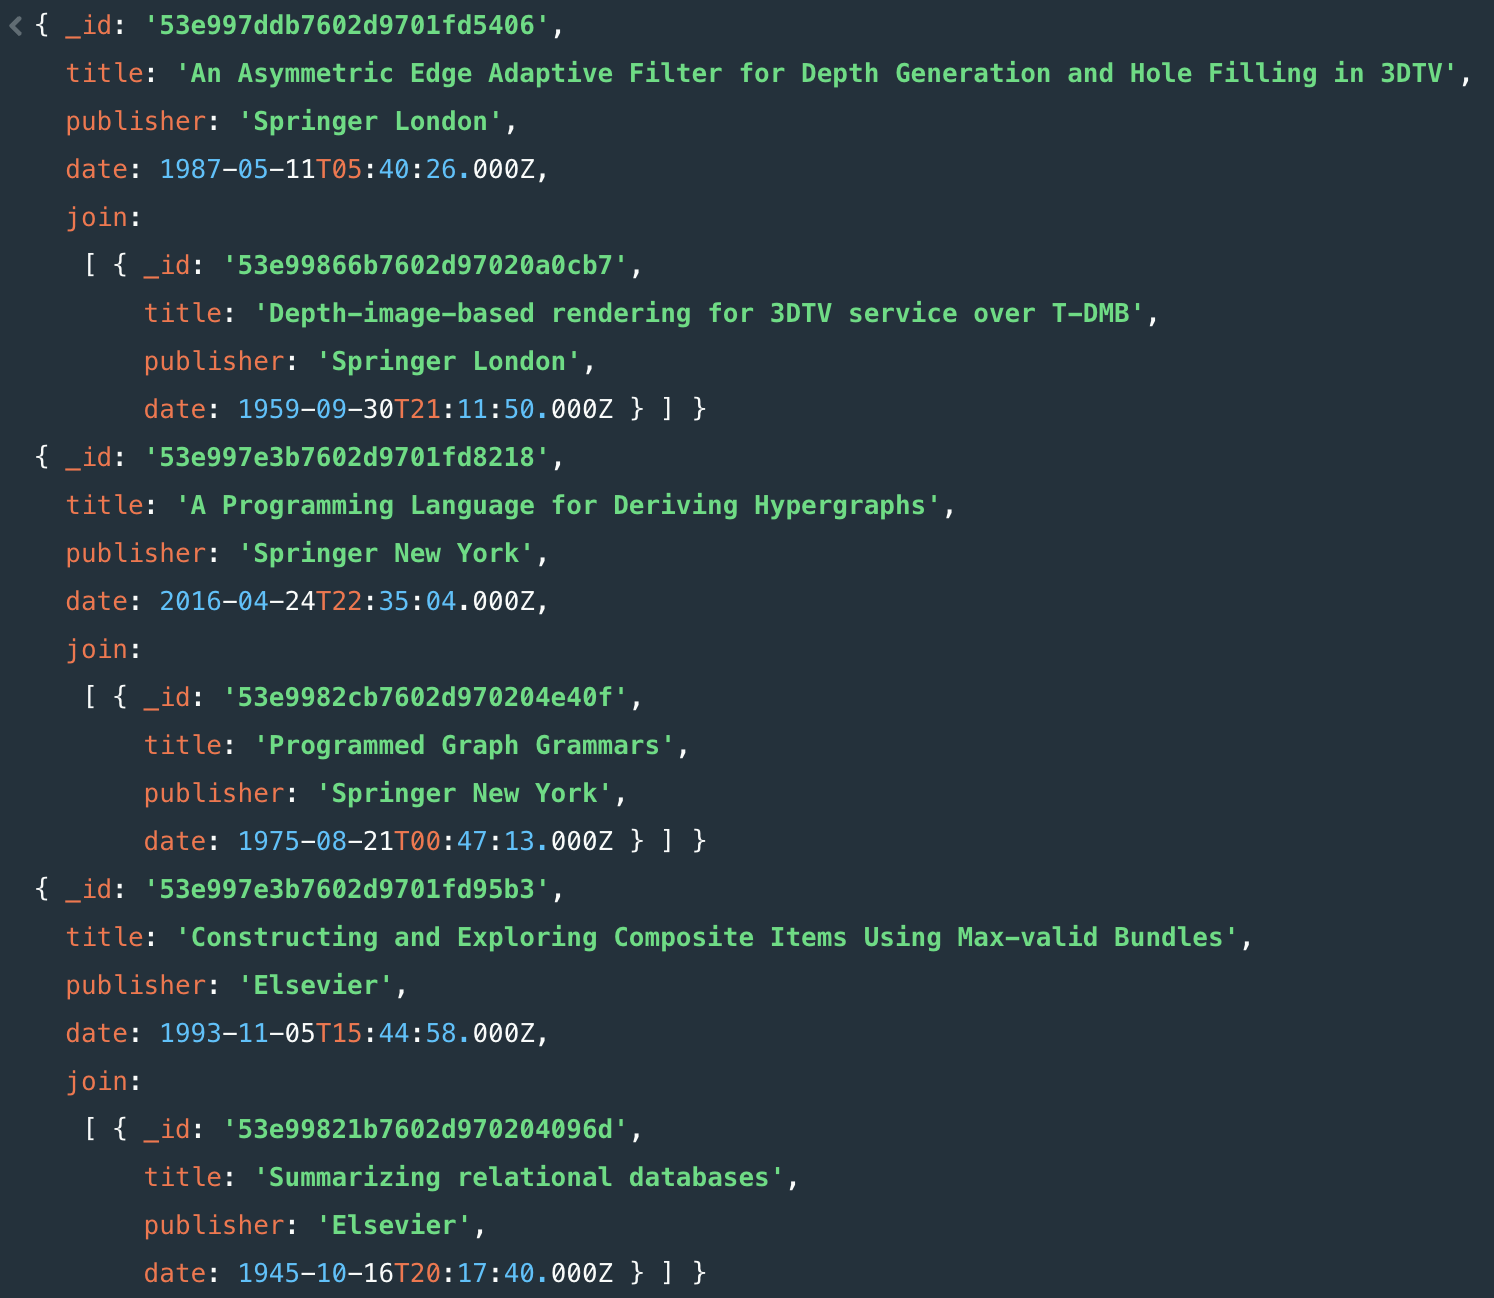
\includegraphics[width=0.9\linewidth]{ImagesMongoDB/query9mongodb}
            \label{fig:query9mongodb}%
        \end{center}
    \end{figure}
    The \verb|$lookup| can be very expensive from a computational point of view and require much time, so to speed the process up it is convenient, when possible, to reduce the input data to the join phase by filtering the documents.
    This can be done by searching for a specific author, title, publisher, or something meaningful in a \verb|$match| condition before the \verb|$lookup|.
    This is possible since all the operations in a query are executed on the database as a pipeline.
    \item \textbf{Recommended books given one book read} \\
    The query returns the book considered the nearest to the given one, in this case, \verb|"Pattern Recognition Letters"|.
    One book is suggested if it has a field of study in common with the book \verb|"Pattern Recognition Letters"|.
    The similarity between books is then evaluated in terms of the number of equal keywords associated with the papers belonging to both considered books.
    \begin{lstlisting}[label={lst:query10mongodb}]
db.bibliography.aggregate( [ {
    $match: { publication_type: "Book" } }, {
    $unwind: { path: "$fos" } }, {
    $unwind: { path: "$keywords" } }, {
    $lookup: {
        from: "bibliography",
        localField: "fos",
        foreignField: "fos",
        as: "otherPaper" } }, {
    $match: { venue: "Pattern Recognition Letters" } }, {
    $unwind: { path: "$otherPaper" } }, {
    $match: { $expr: { $ne: [
        "$_id",
        "$otherPaper._id" ] } } }, {
    $match: { $expr: { $ne: [
        "$venue",
        "$otherPaper.venue" ] } } }, {
    $unwind: { path: "$otherPaper.keywords" } }, {
    $match: { $expr: { $eq: [
        "$keywords",
        "$otherPaper.keywords" ] } } }, {
    $group: {
        _id: { suggestedBook: "$otherPaper.venue" },
        keywordsCount: { $sum: 1 } } }, {
    $sort: { keywordsCount: -1 } }, {
    $limit: 10 }, {
    $project: {
        title: "$suggestedBook",
        similarity: "$keywordsCount" } } ] )
    \end{lstlisting}
    \begin{figure}[H]
        \begin{center}
            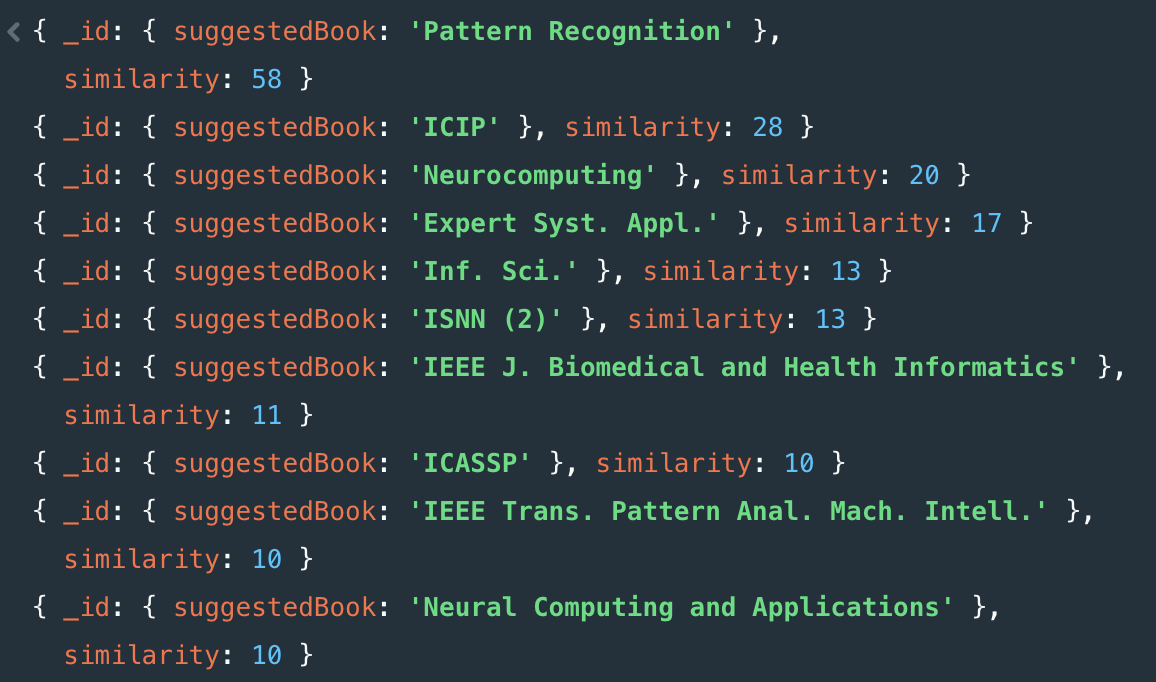
\includegraphics[width=0.9\linewidth]{ImagesMongoDB/query10mongodb}
            \label{fig:query10mongodb}%
        \end{center}
    \end{figure}
    \item \textbf{Authors who have referenced themselves the most within their papers} \\
    The query returns the authors who have referenced themselves the most.
    An author does a self-reference when the considered paper presents a reference to another paper the author has written.
    The results are the name of the authors and the number of times they have made a self-reference, the output is ordered using this number.
    \begin{lstlisting}[label={lst:query11mongodb}]
db.bibliography.aggregate( [ {
    $unwind: { path: "$references" } }, {
    $lookup: {
        from: "bibliography",
        localField: "references",
        foreignField: "_id",
        as: "referencedPaper" } }, {
    $match: { $expr: { $gt: [ {
        $size: "$referencedPaper" }, 0 ] } } }, {
    $unwind: { path: "$referencedPaper" } }, {
    $match: { $expr: { $ne: [
        "$_id",
        "$otherPaper._id" ] } } }, {
    $match: { "authors": { $exists: true } } }, {
    $match: { "referencedPaper.authors": { $exists: true } } }, {
    $unwind: { path: "$authors" } }, {
    $unwind: { path: "$referencedPaper.authors" } }, {
    $match: { $expr: { $eq: [
        "$authors", "$referencedPaper.authors" ] } } }, {
    $group: {
        _id: {
            authorId: "$authors._id",
            authorName: "$authors.name"},
        aut: { $sum: 1 } } }, {
    $sort: {"aut": -1} }, {
    $limit: 10 }, {
    $project: {
        "_id": 0,
        "name": "$_id.authorName",
        "autoreference": "$aut"} } ] )
    \end{lstlisting}
    \begin{figure}[H]
        \begin{center}
            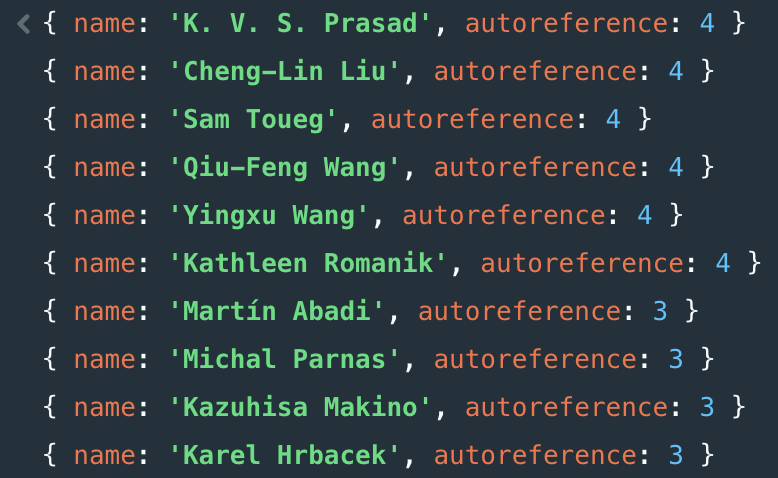
\includegraphics[width=0.6\linewidth]{ImagesMongoDB/query11mongodb}
            \label{fig:query11mongodb}%
        \end{center}
    \end{figure}
\end{enumerate}



    \part{Spark}
    \label{part:spark}%
    \chapter{Introduction to the problem}
\label{ch:introduction_to_the_problem_spark}%
In this part, we implement a bibliographic database relying on the infrastructure provided by Apache Spark.
Apache Spark is a scalable platform for performing complex analytics.
It manages data within a distributed system and this guarantees fast processing, fault tolerance, and high scalability.
The framework allows using different technologies for implementing the database.
We use a logic paradigm that looks like the relational one.
We rely on the \verb|Dataframe| object, which can be imagined as a table containing data but with a lot of enhancing features.
We use \verb|pyspark|, which is the Python library for creating and managing the database in Spark, in order to translate the conceptual model defined in chapter 2.
Articles, authors, and various types of publications become the tables containing the instances of the data.
Apache Spark is a good approach when dealing with huge amounts of data and in the real world, a bibliography database contains a lot of papers.
On the other hand, in our application, we use a small subset of the published papers and we are running Spark only on one machine so we are not fully exploiting the real power of the platform.
In treating this problem from a new point of view, though, we try to take advantage of the functions available in \verb|pyspark| and of its features as much as we can.


\chapter{Dataset structure}
\label{ch:dataset_structure_spark}%
In this part, we implemented a database with a very similar structure to the ER model described in chapter 2.
We decided to create six different tables:
\begin{itemize}
    \item \textbf{df\_papers} is the table containing all the attributes concerning a single paper.
    With respect to the ER model here we have \verb|publication_type| and \verb|publication_id| that are necessary in order to do the join with a certain type of publication; \verb|page_start|; \verb|page_end|; \verb|date| instead of \verb|year|; and \verb|references| which is a list that substitutes the corresponding relationship;
    we also have the lists of \verb|fos| and \verb|keywords| related to the paper and the other attributes identified in the modeling part of the bibliography;
    \item \textbf{df\_aut} is the table related to authors and contains \verb|email| and \verb|bio| in addition to the ER model;
    \item \textbf{df\_aff} is the table with the author's affiliation when the paper was written, this table maps the
    \verb|writes| relationship;
    \item \textbf{df\_journals} is the table with the journals;
    \item \textbf{df\_books} is the table with the books;
    \item \textbf{df\_conferences} is the table with the conferences.

    We decided to represent the entity Publication with the sub-entities, for this reason, all contain \verb|publication_id|  and \verb|publication_type| that are used in the join with \verb|df_papers|.
    The attribute \verb|name| in Publication in the ER model, as well as in other parts of the document, is called \verb|venue|.
\end{itemize}
The following table shows all the fields associated with their respective type, meaning, and table.
\begin{table}[H]
    \begin{center}
        \begin{tabular}{| c | c | c | p{0.25\linewidth} |}
            \hline
            \textbf{Field name} & \textbf{Type}   & \textbf{Description}  & \textbf{Table} \T\B                                      \\
            \hline \hline
            publication\_id     & long            & publication id        & df\_papers, df\_books, df\_journals, df\_conferences\T\B \\
            paper\_id           & string          & paper ID              & df\_papers, df\_aff\T\B                                  \\
            title               & string          & paper title           & df\_papers\T\B                                           \\
            keywords            & array of string & paper keywords        & df\_papers\T\B                                           \\
            fos                 & array of string & paper fields of study & df\_papers\T\B                                           \\
            references          & array of string & paper references      & df\_papers\T\B                                           \\
            page\_start         & integer         & start page            & df\_papers\T\B                                           \\
            page\_end           & integer         & end page              & df\_papers\T\B                                           \\
            lang                & string          & paper language        & df\_papers\T\B                                           \\
            doi                 & string          & paper DOI             & df\_papers\T\B                                           \\
            url                 & array of string & paper URLs            & df\_papers\T\B                                           \\
            abstract            & string          & paper abstract        & df\_papers\T\B                                           \\
            publication\_type   & string          & paper type            & df\_papers\T\B                                           \\
            date                & timestamp       & publication date      & df\_papers\T\B                                           \\
            author\_id          & string          & author ID             & df\_aut, df\_aff\T\B                                     \\
            name                & string          & author name           & df\_aut\T\B                                              \\
            email               & string          & author email          & df\_aut\T\B                                              \\
            bio                 & string          & author short bio      & df\_aut\T\B                                              \\
            organization        & string          & author affiliation    & df\_aff\T\B                                              \\
            venue               & string          & publication name      & df\_books, df\_journals, df\_conferences\T\B             \\
            isbn                & string          & book ISBN             & df\_books\T\B                                            \\
            publisher           & string          & publisher name        & df\_books, df\_journals\T\B                              \\
            volume              & integer         & journal volume        & df\_journals\T\B                                         \\
            issue               & integer         & journal issue         & df\_journals\T\B                                         \\
            issn                & string          & journal ISSN          & df\_journals\T\B                                         \\
            location            & string          & conference location   & df\_conferences\T\B                                      \\
            \hline
        \end{tabular}
        \\[8pt]
        \caption{Description of the fields with related type, meaning, and table.}
        \label{tab:dataset_structure}%
    \end{center}
\end{table}
Below we provide the actual schema of each table obtained by invoking the function \verb|printSchema()|.
\begin{figure}[H]
    \begin{center}
        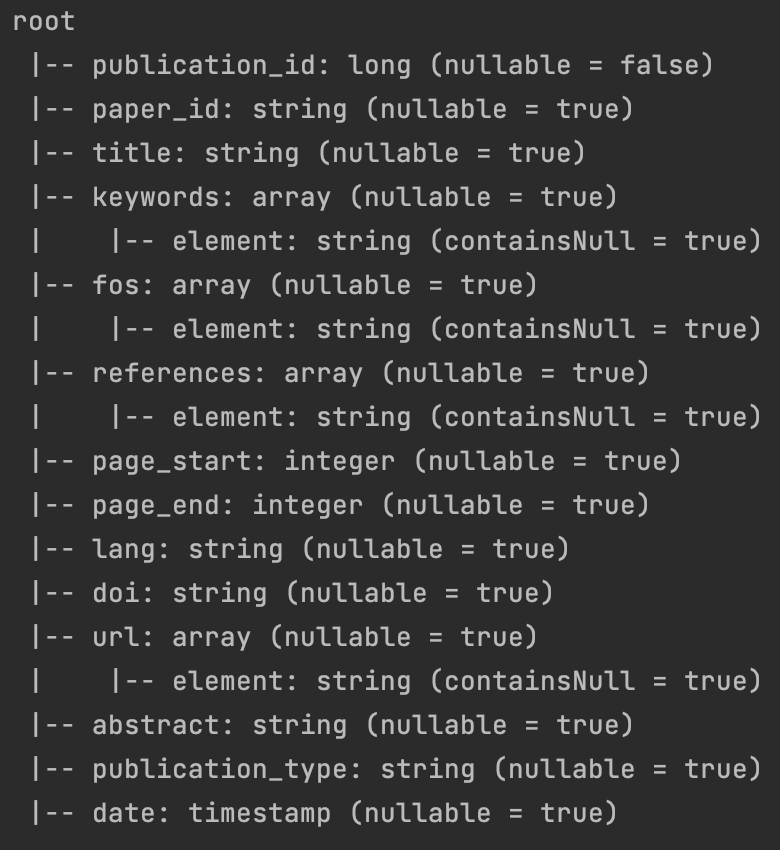
\includegraphics[width=0.6\linewidth]{ImagesSpark/paper_schema}
        \caption{Paper table - df\_papers.}
        \label{fig:figure4_1}%
    \end{center}
\end{figure}
\begin{figure}[H]
    \begin{center}
        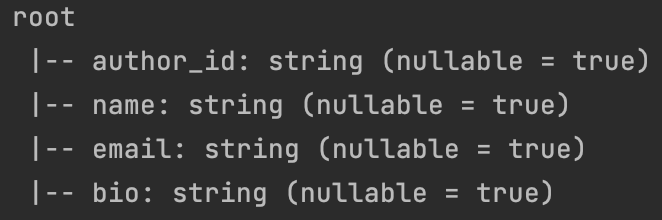
\includegraphics[width=0.6\linewidth]{ImagesSpark/author_schema}
        \caption{Author table - df\_aut.}
        \label{fig:figure4_2}%
    \end{center}
\end{figure}
\begin{figure}[H]
    \begin{center}
        \includegraphics[width=0.6\linewidth]{ImagesSpark/affiliation_schema}
        \caption{Affiliation table - df\_aff.}
        \label{fig:figure4_3}%
    \end{center}
\end{figure}
\begin{figure}[H]
    \begin{center}
        \includegraphics[width=0.6\linewidth]{ImagesSpark/journal_schema}
        \caption{Journal table - df\_journals.}
        \label{fig:figure4_4}%
    \end{center}
\end{figure}
\begin{figure}[H]
    \begin{center}
        \includegraphics[width=0.6\linewidth]{ImagesSpark/book_schema}
        \caption{Book table - df\_books.}
        \label{fig:figure4_5}%
    \end{center}
\end{figure}
\begin{figure}[H]
    \begin{center}
        \includegraphics[width=0.6\linewidth]{ImagesSpark/conference_schema}
        \caption{Conference table - df\_conferences.}
        \label{fig:figure4_6}%
    \end{center}
\end{figure}


\chapter{Data upload}
\label{ch:data_upload_spark}%
The library \verb|pyspark| provides many functions to upload data stored in different formats.
In our case, the dataset was stored in the JSON format, specifically, it is the one used in MongoDB except for some minor changes, so we used the API for this format.
To upload the data we used the object \verb|DataFrameReader|, which is accessible as an attribute of our \verb|SparkSession| instance.
More specifically using the \verb|options| method we specified some instructions on how to read the data, and with the \verb|schema| method we supplied a specific schema for the data to be read in order to keep only the fields specified in it.
We created a DataFrame for each entity of our ER diagram of chapter 2 and we also translated the many-to-may relationship \verb|Writes| into a table to keep track of the \verb|affiliation| field.
For each table, we did some additional filtering on its attributes in order to clean the data and we also did some minor changes that we will now explain.
The dataset we inherited from the MongoDB part had a simple structure: a single document, the paper, where all other entities (authors, publication, affiliation) were stored as sub-documents, a collection of sub-documents or simple fields that are present only when needed.
Therefore, we have to extrapolate the information regarding the authors and the publications from the papers.
In particular, a more complex process was applied to build the dataframes containing information concerning books, conferences, and journals.
The following sections briefly explain the processing done within the upload step for each entity contained in the spark database and the reasoning behind it.


\section{Author table}
\label{sec:author_table_spark}%
This table was created by extracting from each Paper document the array containing the authors' documents, with their fields.
To do this, we first had to load the data using the load process described in the section before.
Secondly, we unwrapped each array using the \verb|explode| function to have a table where each row represents the author document.
Finally, we did some filtering on null values and some minor operations, such as renaming, deleting duplicates, or dropping columns.


\section{Paper, Book, Conference, Journal tables}
\label{sec:paper_book_conference_journal_tables}%
To load the data relevant to the entities Book, Conference, and Journal we had to address two issues: how to extract and integrate the different types of publications and how to link each paper to the publication medium in which it was published.
The first issue is solved by uploading in the DataFrame of each publication type only the fields regarding that specific entity, namely the attributes present in the ER model of section 2, and filtering each DataFrame removing the duplicate rows.
We also imposed that the fields have to be not null.
To overcome the second issue we opted to introduce a ``foreign key'' column in the paper DataFrame which stores the unique identifier of the publication medium where it was published.
To make the linking with the ``foreign key'' approach work, we added a unique identifier to each single publication instance cleaned through the previous step.
This identifier is generated using a hashing function, specifically the function \verb|xxhash64| present in the pyspark library, which uses the 64-bit variant of the xxHash algorithm.
We fed this function with the columns we identified as the primary key, to generate the unique identifier.

The other possible solution we thought of was the creation of an array inside each publication containing all the papers present inside it.
In the end, we adopted the first solution because our focus is on the paper, which is the main entity of the database and we assume that the vast majority of the queries will probably have the paper as a starting point, and then retrieve all the information correlated to the paper.
In this way, opting for the first solution and considering the assumption mentioned here, the queries done on the papers should be more efficient.

The process we used to upload Books, Journals and Conferences is the following:
\begin{enumerate}
    \item Upload the paper documents from the JSON input file in a DataFrame with the structure we defined in chapter 12, except for the attribute \verb|publication_id| that will be added later;
    \item For each type of publication:
    \begin{enumerate}
        \item Upload the data from the JSON file keeping only the fields relative to a single publication type and the field \verb|_id|, which is the identifier of a paper;
        \item Filter out the rows of the dataframe which have the publication's identifying fields set to null, namely \verb|('venue', 'volume', 'issue', 'issn')| for the journals, \verb|('isbn', 'venue')| for the books and \verb|('venue')| for the conferences;
        \item Group each publication by the uniquely identifying fields and collect the the other fields, especially \verb|_id|, in lists;
        \item Select the first element of the list of non-identifying attributes, \verb|'publisher'| for journals and books, and \verb|'location'| for the conferences.
        This choice is motivated by the fact that these fields were set using random strings extracted from some datasets we found on the web.
        In real scenarios, where we assume to have meaningful data, the best thing to do would be to implement a strategy that keeps the last inserted value for the field or the one that appears the most;
        \item Create the publication identifier (field \verb|publication_id|) using the previous explained hash function;
        \item Create a new DataFrame containing papers, constructed by joining the previous imported Paper DataFrame (Point 1) with the DataFrame of the publication on the field \verb|_id|, which is the paper identifier.
        In this way we attach to the newly generated Paper DataFrame the \verb|publication_id| field, linking the paper to it's publication.
        Notice that in order to perform the join we first have to \textit{explode} the field \verb|_id| of the publication DataFrame;
    \end{enumerate}
    \item At this step of the process, in addition to the dataframes for the journals, for the books and for the conferences we also have other the three newly created paper dataframes obtained by the joining operations.
    These lastly mentioned dataframes have the same structure of the originial one with the addition of the fields that identify the paper publication.
    By merging this the three dataframes we obtain the final dataframe of the papers.
\end{enumerate}
In addition to this major operation some minor ones were performed, such as renaming or dropping columns, but these are straightforward to understand, so we won't discuss them any further in this report.


\section{Affiliation table}
\label{sec:affiliation_table}%
This table was created by uploading, from the JSON file, only the identifiers of the papers and their array of authors keeping the id of the author and the organization to which they were affiliated.
After filtering the null values, the authors' array is expanded, using the \verb|explode()| function.
As before, some other minor operations were also done, such as renaming or dropping of columns.


\chapter{Commands and queries}
\label{ch:commands_and_queries_spark}%


\section{Commands}
\label{sec:commands_spark}%

\begin{enumerate}
    \item \textbf{Add a new paper to the DataFrame} \\
    With this command, we want to show how to add a new row to our Paper DataFrame.
    In our example, we suppose that the paper has been saved in a JSON file and has a structure consistent with the schema defined in chapter 12 for the input dataset.
    This way, we can reuse the loading procedure used before for the entire dataset loading.
    We first create a new DataFrame for the single paper.
    Once the paper is loaded, we can proceed to extract other information relevant to the paper, like the authors, and the publication medium but we don't show this part here to have a more concise description (the actual implementation is present on the notebook).
    After this operation, we proceed to insert the foreign\_key associated with the publication medium in the DataFrame containing our paper to insert.
    This operation is done using the \verb|select| method so we can insert the column as the first one to stay uniform with the structure because in spark even the order of the columns is important.
    To create the column from a literal value we use the function \verb|lit|.
    Now the new paper is ready to be added, we have only to first check if the paper is already present in the DataFrame, and we do this by filtering by \verb|paper_id| and verifying that the collection is empty.
    Then to add the paper we use the method \verb|union| which is applied to DataFrame and returns a new DataFrame containing the union of rows of both DataFrames.
    \begin{lstlisting}[label={lst:command1spark}]
new_paper_file = 'single_paper.json'

new_paper = spark.read.options(**OPTIONS)
.json(new_paper_file, schemaPaper)\
.withColumnRenamed("_id", "paper_id")

# Other code for loading publication, authors, etc
# ...

# Inserting foreign_key at position 0
new_paper = new_paper.select(lit(foreign_key).alias('publication_id'), '*')

paper_id = new_paper.head(1)[0].asDict()['paper_id']

if df_papers.filter(col('paper_id') == paper_id).collect() == []:
df_papers = df_papers.union(new_paper)
    \end{lstlisting}
    \item \textbf{Update one single row of a dataframe or multiple rows} \\
    The word update has to be intended as the creation of a new dataframe instance which is generated from the previous data changed in the way we want.
    Indeed, the Dataframe data structure, available in Spark, is immutable so it cannot be modified.
    Since the modifications are not allowed, to update a single entry the process is a little longer than the one used on other databases.

    The update process can be useful for uploading papers when new data enter the database or when parts of the data were wrong and need to be corrected.
    There may be many handmade ways to update a dataframe since there are no standard methods.
    All of them are similar in their underlying idea.

    The command modifies the DOI and URL of a paper with an identifier equal to \verb|'53e997e4b7602d9701fdb48a'|.
    For doing this operation we first filter the dataframe keeping only the row to be modified.
    We add a column for each value we want to insert under the name \verb|new_fieldName|.
    Then we drop the old columns containing the previous values and we rename the new columns with the name of the old ones.
    Finally, we make the union between the entire dataframe, without the row we want to modify, and the new entry.
    The \verb|union| function allows to merge two DataFrame with the same schema;
    if the two structures are different, then the function gives an error.

    The function \verb|lit| is used for creating a new column containing a literal, namely a constant value.
    The function \verb|array| is used for creating a new array column.
    \begin{lstlisting}[label={lst:command2spark}]
from pyspark.sql.functions import lit, array

updated_df_papers = df_papers\
.filter(col('paper_id') == '53e997e4b7602d9701fdb48a')
updated_df_papers = updated_df_papers\
.withColumn('new_doi', lit('10.1007/11944577_37'))\
.withColumn('new_url', array([lit('https://link.springer.com/chapter/10.1007/11944577_37')]))
updated_df_papers = updated_df_papers\
.drop(col('doi')).drop(col('url'))\
.withColumnRenamed('new_doi', 'doi')\
.withColumnRenamed('new_url', 'url')

updated_df_papers = df_papers.filter(col('paper_id') != '53e997e4b7602d9701fdb48a').union(updated_df_papers)
updated_df_papers.filter(col('paper_id') == '53e997e4b7602d9701fdb48a').select('paper_id', 'title', 'doi', 'url').show(truncate = False)
    \end{lstlisting}
    An analogous method can be applied when we want to update multiple rows following some rule.
    In this case, the filter will keep many rows and not just one.
    \begin{figure}[H]
        \begin{center}
            \includegraphics[width=0.9\linewidth]{ImagesSpark/command2spark}
            \label{fig:command2spark}%
        \end{center}
    \end{figure}
    \item \textbf{Remove an entire column} \\
    In Spark, we can remove an entire column from a data frame due to deleting information that is no more informative.
    In these cases, we delete them to free memory for new data.

    To realize our objective, we use the function \verb|drop|, which removes entirely values associated with a field of the data frame.

    In our database, we can use the explained function over the column \verb|lang| because we have realized that all the papers have the same value, \verb|en|.
    Then, we print the schema of the data frame to see if the function ran properly.
%and finally, we visualize an example of the new paper by calling the \verb|show| operation.
    \begin{lstlisting}[label={lst:command3spark}]
df_papers_without_lang = df_papers \
.drop('lang')

df_papers_without_lang.printSchema()
df_papers_without_lang.show(1)
    \end{lstlisting}
    \begin{figure}[H]
        \begin{center}
            \includegraphics[width=0.6\linewidth]{ImagesSpark/command3spark}
            \label{fig:command3spark}%
        \end{center}
    \end{figure}
    \item \textbf{Delete all the papers published before a certain year} \\
    In order to delete from the DataFrame \verb|df_papers| the rows that represent papers published before a certain year is necessary to create a new DataFrame extracting from the original one only the papers that satisfy the desired condition.
    We decided to remove all the papers that were published before the \verb|1950| because we consider them obsolete.
    To check the year in which a paper was published is necessary to use the function \verb|year| in order to extract the information from the \verb|date|, that is of type \verb|TimeStamp|.
    Based on the condition \verb|year('date') > '1950'| we drop with the \verb|where| clause all the rows that do not satisfy it, saving all the others in the new DataFrame.
    Finally, with the following command, we show the result of these actions and we present the new \verb|df_papers| ordering the visualization by date, so it is immediately visible that there are no papers realized before \verb|1951|.
    \begin{lstlisting}[label={lst:command4spark}]
from pyspark.sql.functions import year

df_papers = df_papers\
.filter(year('date') > '1950')

df_papers.select('title', 'publication_type', 'date')\
.orderBy('date')\
.show(truncate = False)
    \end{lstlisting}
    \begin{figure}[H]
        \begin{center}
            \includegraphics[width=0.9\linewidth]{ImagesSpark/command4spark}
            \label{fig:command4spark}%
        \end{center}
    \end{figure}
    \item \textbf{Create a new column with the paper's total number of pages} \\
    With this command, we create a new DataFrame \verb|df_papers_total_pages| starting from \verb|df_papers| but with an additional column called \verb|total_pages| using the function \verb|withColumn()|.
    This new column contains the total number of pages of the paper computed as the difference between \verb|pages_end| and \verb|page_start| by doing also some consistency checks on these values.
    Then only some fields are displayed just for better reading.
    \begin{lstlisting}[label={lst:command5spark}]
df_papers_total_pages = df_papers \
.filter((col('page_start') >= 0) & (col('page_end') >= 0) & (col('page_start') <= col('page_end'))) \
.withColumn('total_pages', col('page_end') - col('page_start'))

df_papers_total_pages \
.select(col('title'), col('page_start'), col('page_end'), col('total_pages')) \
.show(5, truncate=False)
    \end{lstlisting}
    \begin{figure}[H]
        \begin{center}
            \includegraphics[width=0.9\linewidth]{ImagesSpark/command5spark}
            \label{fig:command5spark}%
        \end{center}
    \end{figure}
\end{enumerate}


\section{Queries}
\label{sec:queries_spark}%
\begin{enumerate}
    \item \textbf{Retrieve all papers published on a specific issue and volume of a Journal} \\
    With this simple query, we want to retrieve all the papers published on a specific issue and on a specific volume of a specific Journal.
    The specifics of the journal are saved in variables to be used later.
    To perform the query we first do a filtering (which is equivalent to a \verb|WHERE|) on the DataFrame containing the journals, to extract only the row concerned with our paper.
    After that, we perform the default \verb|inner| join with the papers' DataFrame.
    Notice that, besides specifying the column on which to perform the join, we do an additional check on the \verb|publication_type| to ensure that the join operations are done only for journals.
    This type of checking is made easy thanks to the possibility offered by Spark to specify more complex join conditions.
    \begin{lstlisting}[label={lst:query1spark}]
venue, volume, issue = ('BMC Bioinformatics', '14', '1')

df_papers_q1 = df_journals\
.filter((col('venue') == venue) &
(col('volume') == volume) &
(col('issue') == issue))\
.join(df_papers,
(df_journals['publication_id'] == df_papers['publication_id']) &
(df_papers['publication_type'] == 'Journal')
)

df_papers_q1.select(['paper_id', 'title']).show(truncate=60)
    \end{lstlisting}
    \begin{figure}[H]
        \begin{center}
            \includegraphics[width=0.9\linewidth]{ImagesSpark/query1spark}
            \label{fig:query1spark}%
        \end{center}
    \end{figure}
    \item \textbf{Papers written in the last 20 years and containing a chosen string within a keyword} \\
    Find the papers written in the last twenty years whose keywords contains at least one keyword having \verb|artificial| as substring.
    We require that these papers have the DOI set to a not null value.
    The results are ordered ascending by the date and only 15 elements are printed.

    For filtering a Dataframe variable we can use the function \verb|filter(condition)| of \verb|pyspark| library.
    This function returns a new DataFrame containing only the rows which make the condition true and eliminate the others.
    We can use the function \verb|like(string)| as a filtering condition on a column of the DataFrame for keeping only the rows whose considered attribute contains the substring passed as parameter.
    The \verb|sort| functions can be used for ordering the rows of the DataFrame using the field passed as an argument to the function.
    The limit function is used for keeping only the first fifteen rows of the dataframe.
    The function \verb|current_timestamp| returns the timestamp in the current instant.
    Here the computation of the number of years, needed for passing from is done without considering leap years for simplicity.
    \begin{lstlisting}[label={lst:query2spark}]
df = df_papers.withColumn('current time', current_timestamp())
df \
.filter((((unix_timestamp('current time') - unix_timestamp('date')) / 3600 / 24 / 365) < 20) &
(col('doi').isNotNull())) \
.select('paper_id',
'title',
'date',
explode('keywords').alias('keyword')) \
.filter(col('keyword').like('%artificial%')) \
.distinct() \
.select('title',
'date',
'keyword') \
.sort(col('date').asc()) \
.limit(15) \
.show(truncate=55)
    \end{lstlisting}
    \begin{figure}[H]
        \begin{center}
            \includegraphics[width=0.9\linewidth]{ImagesSpark/query2spark}
            \label{fig:query2spark}%
        \end{center}
    \end{figure}
    \item \textbf{Retrieve papers published in conferences that have topics about multiagent systems} \\
    This query retrieves the papers with \verb|multiagent system| within its keywords, so we are interested only in a subset of our database.
    In extracting them, we select at first some of the columns of the dataframe associated with papers, and in particular, we call the explode function over the \verb|keywords| column to duplicate the rows and associate to them an element of the exploded column.
    Then, we extract a subset of all the generated rows by selecting only those that have as keyword \verb|multiagent system|.
    We extract only the columns \verb|title|, \verb|publication_type|, \verb|paper_id|, \verb|publication_id|, and \verb|date|, and we save the result in a variable called \verb|nested_query|.

    Thus, we perform another query over the created dataframe by first calling a join operation to join it with the one associated with the conferences, matching the variable \verb|publication_id|, and then we select only those papers of interest.
    We reorder the rows by date in a descending way, and then we extract only the title of the paper and the venue of the conference.
    Finally, we show the dataframe obtained.
    \begin{lstlisting}[label={lst:lstlisting4_1_8}]
nested_query = df_papers \
.select('title',
'publication_type',
'paper_id',
'publication_id',
'date',
explode('keywords').alias('keyword')) \
.filter(col('keyword').isin('multiagent system')) \
.drop('keyword')
df_conferences \
.join(nested_query, 'publication_id') \
.filter(col('publication_type') == 'Conference') \
.orderBy('date', ascending=False) \
.select(col('title').alias('paper title'),
col('venue').alias('conference venue')) \
.show(5, truncate=50)
    \end{lstlisting}
    \begin{figure}[H]
        \begin{center}
            \includegraphics[width=0.9\linewidth]{ImagesSpark/query3spark}
            \label{fig:query3spark}%
        \end{center}
    \end{figure}
    \item \textbf{Retrieve the most prolific organizations regarding the conferences} \\
    This query tries to retrieve the organizations that published more than \verb|10| conferences, so the most prolific ones in these kinds of publications.
    We first execute a join between the DataFrame that contains the papers and the one that contains the affiliations, because to obtain the result we need information from them both.
    We need to filter on the \verb|publication_type| that is present in \verb|df_papers| in order to consider only the conferences and, then, we group by \verb|organization|, present in the \verb|df_aff|, and with \verb|collect_set()| we collect for each organization the list of the related papers, avoiding duplicates.
    Finally, we filter the result, retrieving only those organizations whose associated list has more than \verb|10 paper_id|.
    In showing the most prolific organizations we truncate the columns' text using \verb|truncate = 50|, to have a compact and clear visualization.
    \begin{lstlisting}[label={lst:query4spark}]
from pyspark.sql.functions import collect_set, size

df_aff \
.join(df_papers, df_papers.paper_id == df_aff.paper_id, 'inner') \
.drop(df_papers.paper_id) \
.select('paper_id',
'organization',
'publication_type') \
.filter((col('organization').isNotNull()) &
(col('organization') != "") &
(col('publication_type') == "Conference")) \
.groupBy('organization') \
.agg(collect_set('paper_id').alias('papers')) \
.filter(size(col('papers')) > 10) \
.show(truncate=50)
    \end{lstlisting}
    \begin{figure}[H]
        \begin{center}
            \includegraphics[width=0.9\linewidth]{ImagesSpark/query4spark}
            \label{fig:query4spark}%
        \end{center}
    \end{figure}
    \item \textbf{Retrieve some statistics about papers } \\
    In this query, we retrieve some statistics about papers published from the year 2015 on.
    We group the articles by publication year using the \verb|year()| function to extract the year from the date.
    Then some aggregate functions are performed to obtain insights like the total number of papers published using \verb|count()|, the total number of pages written, the minimum and the maximum number of pages in an article using \verb|sum()|, \verb|min()|, \verb|max()| and lastly the mean of pages written per article and the variance using \verb|avg()| and \verb|variance()|.
    To round the fractional numbers we use \verb|format_number()|.
    Years are shown in decreasing order.
    In this query we use the DataFrame obtained by running the command 5.
    \begin{lstlisting}[label={lst:query5spark}]
from pyspark.sql.functions import sum, min, max, avg, format_number, variance

df_papers_total_pages \
.filter(year(col('date')) >= 2015) \
.groupBy(year(col('date')).alias('year')) \
.agg(count('paper_id').alias('total_papers'),
sum('total_pages').alias('total_pages'),
min('total_pages').alias('min_pages'),
max('total_pages').alias('max_pages'),
format_number(avg('total_pages'), 2).alias('avg_pages'),
format_number(variance('total_pages'), 2).alias('var_pages')) \
.sort(col('year').desc()) \
.show()
    \end{lstlisting}
    \begin{figure}[H]
        \begin{center}
            \includegraphics[width=0.9\linewidth]{ImagesSpark/query5spark}
            \label{fig:query5spark}%
        \end{center}
    \end{figure}
    \item \textbf{Papers that are referenced the most and have at least 30 references} \\
    With this query, we want to know which papers present in our DB are referenced the most absolute ly.
    We achieve this goal by first unwrapping the references for each paper using the \verb|explode| function.
    Then, we proceed grouping by the reference we previously \textit{exploded} and use the \verb|count| aggregation function to actually count the papers who have that particular reference, saving this value in the column \verb|references_count|.
    Lastly, we do a filtering on \verb|references_count| to extract only the papers with at least 30 references, and a join to get some significant data about the papers we extracted with the previous operations.
    \begin{lstlisting}[label={lst:query6spark}]
df_papers \
.select('paper_id',
'title',
explode(col('references')).alias('reference')) \
.groupBy('reference') \
.agg(count('paper_id').alias('references_count')) \
.filter(col('references_count') > 30) \
.join(df_papers, col('reference') == df_papers.paper_id) \
.sort(col('references_count').desc()) \
.select(['title', 'references_count']) \
.show(truncate=50)
    \end{lstlisting}
    \begin{figure}[H]
        \begin{center}
            \includegraphics[width=0.9\linewidth]{ImagesSpark/query6spark}
            \label{fig:query6spark}%
        \end{center}
    \end{figure}
    \item \textbf{Couples of the field of study and keywords which appear more frequently within the papers} \\
    The query returns the association between fields of study and keywords which are more present inside the database and how many times they appear together.
    Initial filtering is done in order to eliminate the papers which don't contain any keyword or field of study.
    The two clauses for doing the filtering can be modified by increasing the required number of keywords or the required number of fields of study.
    This kind of change can be interesting in order to understand which fields of study and keywords become more relevant when the subset of the considered paper is different.
    The results are ordered by the number of occurrences of the couples \verb|field of study| - \verb|keyword| by decreasing order.
    We filter out the couples of fields of study and keywords with less than 100 occurrences in order to get rid of some misleading information due to not coupled elements.
    The threshold can be adjusted.
    \begin{lstlisting}[label={lst:query7spark}]
from pyspark.sql.functions import year, col, size

df = df_papers \
.filter(
(col('doi').isNotNull()) &
(year(col('date')) >= 2000) &
(size(col('fos')) > 0) &
(size(col('keywords')) > 0)) \
.select('fos', explode('keywords').alias('keyword')) \
.select('keyword', explode('fos').alias('fos')) \
.groupby('fos', 'keyword') \
.count() \
.withColumnRenamed('count', 'couple count') \
.filter(col('couple count') > 100) \
.sort(col('couple count').desc()) \
.limit(15) \
.show(truncate=False)
    \end{lstlisting}
    \begin{figure}[H]
        \begin{center}
            \includegraphics[width=0.9\linewidth]{ImagesSpark/query7spark}
            \label{fig:query7spark}%
        \end{center}
    \end{figure}
    \item \textbf{Retrieve the organizations associated with an author name for each field of study} \\
    For each field of study associated with papers written by any author named \verb|Hao Wang|, this query retrieves all the organizations that have contributed to that field of study through the searched authors.

    For the complexity of the problem, we split the query into two nested queries.
    At first, we query the data frame associated with authors by filtering it to extract the author \verb|Hao Wang|.
    Then we select only the \verb|author_id| column, and we collect the values in a list called \verb|sub_nested_query| through the functions \verb|flatMap| and \verb|collect|.

    Next, we are interested in filtering also the data frame associated with affiliation by extracting rows that have \verb|author_id| present inside the \verb|sub_nested_query| list.
    We also filter the same data frame by extracting only the rows with a not-null value of the organization column, and then we assign the result to the \verb|nested_query| variable.

    Finally, we join over the column \verb|paper_id| the last result with the data frame associated with papers.
    From the joined data frame, we explode the column \verb|fos|, and we associate to each of those elements called \verb|field_of_study| the value of the columns \verb|paper_id| and \verb|organization|.
    We group the rows by the \verb|field_of_study| values, and then we aggregate through the function \verb|agg| the organizations that are collected in a set by the last operation.
    We are performing these operations because we are interested in all the organizations in which the author has worked in his carrier.
    In the end, we rearrange the rows by ordering the column \verb|field_of_study| alphabetically.
    \begin{lstlisting}[label={lst:query8spark}]
author_name = 'Hao Wang'

sub_nested_query = df_aut \
.filter(col('name') == author_name) \
.select('author_id') \
.rdd.flatMap(lambda x: x) \
.collect()

nested_query = df_aff \
.filter(col('author_id').isin(sub_nested_query)) \
.filter(col('organization') != 'null')

df_papers \
.join(nested_query, 'paper_id') \
.select('paper_id',
'organization',
explode('fos').alias('field_of_study')) \
.groupBy('field_of_study') \
.agg(collect_set('organization').alias('organization')) \
.orderBy('field_of_study') \
.show(14, truncate=80)
    \end{lstlisting}
    \begin{figure}[H]
        \begin{center}
            \includegraphics[width=0.9\linewidth]{ImagesSpark/query8spark}
            \label{fig:query8spark}%
        \end{center}
    \end{figure}
    \item \textbf{Retrieve the most prolific publishers} \\
    In this query, we join the \verb|df_books| and the \verb|df_journals| on the \verb|publisher| column.
    Due to this join and to the fact that the two DataFrames have both the column \verb|venue| we have to rename this column in at least one of the tables, to have distinguishable data.
    We decided to rename both columns to have more clear data in the new DataFrame, created by the join operation.
    In this case, combining the related tuples from books and journals, we are interested only in journals' publications that arrived at least at volume \verb|10|, while we consider all the books without filtering them.
    After the execution of the join, we drop the duplicates and group them by \verb|publisher|.
    Then, we create two sets related to the publisher, one for the books and one for the journals, and we concatenate them to obtain for each publisher a single list with all its publications.
    We define sets and not lists because they don't allow to have duplicates of values.
    Now, we can retrieve the most prolific publishers, just by filtering on the size of the list of publications associated with the publishers.
    In our dataset, there are not a lot of publishers that have more than \verb|500| publications, so these are the most prolific ones, but the filtering can be modified at any time, depending on the data, to obtain meaningful results.
    \begin{lstlisting}[label={lst:query9spark}]
from pyspark.sql.functions import collect_set, concat, size

df_journals \
.withColumnRenamed('venue', 'venueJournals') \
.filter((col('volume')) > 10) \
.join(df_books, df_books.publisher == df_journals.publisher, 'inner') \
.drop(df_journals.publisher) \
.withColumnRenamed('venue', 'venueBooks') \
.select('venueBooks',
'venueJournals',
'publisher') \
.dropDuplicates(['venueBooks',
'venueJournals',
'publisher']) \
.groupBy('publisher') \
.agg(collect_set('venueBooks').alias('books'),
collect_set('venueJournals').alias('journals')) \
.withColumn('total_publications_per_publisher', concat('books', 'journals')) \
.filter(size('total_publications_per_publisher') > '500') \
.select('publisher',
'total_publications_per_publisher') \
.show(truncate=50)
    \end{lstlisting}
    \begin{figure}[H]
        \begin{center}
            \includegraphics[width=0.9\linewidth]{ImagesSpark/query9spark}
            \label{fig:query9spark}%
        \end{center}
    \end{figure}
    \item \textbf{Prolific authors with different organizations} \\
    The query retrieves authors who worked for at least three different organizations and have published at least three papers with at least five fields of study and five references each.
    To obtain this it is necessary to join the paper table with the affiliation DataFrame on \verb|paper_id| and then join it with the author DataFrame on \verb|author_id|.
    We group on \verb|author_id| to get all the aggregate information for each author.
    To count the different organizations an author has worked for we use \verb|approx_count_distinct()|, which gives a faster response counting approximately the different values, if interested in the exact value it is possible to use \verb|countDistinct()|.
    In the \verb|HAVING| part, for consistency, we check that only one name is associated with the grouped \verb|author_id| and in the \verb|SELECT| part we explode that field to obtain a single string instead of an array.
    The result is decreasingly ordered by the number of papers and then the number of organizations.
    \begin{lstlisting}[label={lst:query10spark}]
from pyspark.sql.functions import approx_count_distinct

df_papers \
.filter((size(col('fos')) >= 5) &
(size(col('references')) >= 5)) \
.join(df_aff, df_papers.paper_id == df_aff.paper_id, 'inner') \
.drop(df_aff.paper_id) \
.join(df_aut, df_aff.author_id == df_aut.author_id, 'inner') \
.drop(df_aff.author_id) \
.groupBy('author_id') \
.agg(count('paper_id').alias('papers_count'),
approx_count_distinct('organization').alias('organizations_count'),
collect_set('name').alias('name')) \
.filter((size('name') == 1) &
(col('papers_count') >= 3) &
(col('organizations_count') >= 3)) \
.orderBy(col('papers_count').desc(),
col('organizations_count').desc()) \
.select(explode('name').alias('name'),
'papers_count',
'organizations_count') \
.show(5)
    \end{lstlisting}
    \begin{figure}[H]
        \begin{center}
            \includegraphics[width=0.9\linewidth]{ImagesSpark/query10spark}
            \label{fig:query10spark}%
        \end{center}
    \end{figure}
\end{enumerate}

    \begin{thebibliography}{1}
        \bibitem{github_reference} \textbf{GitHub repository that contains all the scripts mentioned in the document} \href{https://github.com/IrfEazy/smbud-project}{www.github.com/IrfEazy/smbud-project}
    \end{thebibliography}
\end{document}
